% Para utilizar este template siga o tutorial disponível em http://www.biblioteca.ufc.br/images/arquivos/instrucoes_modelos/tutorial_sharelatex.pdf

%%%%%%%%%%%%%%%%%%%%%%%%%%%%%%%%%%%%%%%%%%%%%%%%%%%%%%%
%% Você dever criar uma conta no ShareLatex. Depois, %%
%% vá nas opções no canto esquerdo superior da tela  %%
%% e clique em "Copiar Projeto". Dê um novo nome pa- %%
%% ra o projeto.                                     %%
%%                                                   %%
%% Os principais desenvolvedores deste template são: %%
%%                                                   %%
%%            Ednardo Moreira Rodrigues              %%
%%     (Doutorando em Engenharia Elétrica - UFC)     %%
%%                      &                            %%
%%            Alan Batista de Oliveira               %%
%%     (Graduando em Engenharia Elétrica - UFC)      %%
%%                                                   %%
%% Revisão:                                          %%
%%                                                   %%
%% - Eliene Maria Vieira de Moura;                   %%
%% - Francisco Edvander Pires Santos;                %%
%% - Izabel Lima dos Santos;                         %%
%% - Juliana Soares Lima;                            %%
%% - Kalline Yasmin Soares Feitosa.                  %%
%%                                                   %%
%% Colaborador:                                      %%
%% -Andrei Bosco Bezerra Torres                      %% 
%% (Professor - Sistemas e Mídias Digitais -         %%
%% Instituto Universidade Virtual - UFC)             %%
%%                                                   %%
%% Grande parte do trabalho foi adaptado do template %%
%% da UECE elaborado por:                            %%
%% Thiago Nascimento  (UECE)                         %%
%% Project available on:                             %%
%% https://github.com/thiagodnf/uecetex2             %%
%%                                                   %%
%% "Dúvidas, esclarecimentos ou sugestões podem ser  %%
%% enviadas para o e-mail da Comissão de Serviços da %%
%% Biblioteca Universitária: csbu@ufc.br."           %%
%%                                                   %%
%% As últimas atualizações estão descritas no inicio %%
%% do arquivo "README.md".                           %%
%%                                                   %%
%%%%%%%%%%%%%%%%%%%%%%%%%%%%%%%%%%%%%%%%%%%%%%%%%%%%%%%

\documentclass[        
    a4paper,          % Tamanho da folha A4
    12pt,             % Tamanho da fonte 12pt
    chapter=TITLE,    % Todos os capitulos devem ter caixa alta
    section=Title,    % Todas as secoes devem ter caixa alta somente na primeira letra
    subsection=Title, % Todas as subsecoes devem ter caixa alta somente na primeira letra
    oneside,          % Usada para impressao em apenas uma face do papel
    english,          % Hifenizacoes em ingles
    spanish,          % Hifenizacoes em espanhol
    brazil,           % Ultimo idioma eh o idioma padrao do documento
    fleqn             % Coloca as equações alinhadas a esquerda
]{abntex2}

% Para utilizar este template siga o tutorial disponível em http://www.biblioteca.ufc.br/wp-content/uploads/2015/09/tutorial-sharelatex.pdf

%%%%%%%%%%%%%%%%%%%%%%%%%%%%%%%%%%%%%%%%%%%%%%%%%%%%%%%
%% Você deve criar uma conta no Overleaf. Depois,    %%
%% vá nas opções no canto esquerdo superior da tela  %%
%% e clique em "Copiar Projeto". Dê um novo nome pa- %%
%% ra o projeto.                                     %%
%%                                                   %%
%% Os principais desenvolvedores deste template são: %%
%%                                                   %%
%%            Ednardo Moreira Rodrigues              %%
%%       (Doutor em Engenharia Elétrica - UFC)       %%
%%(Coord. do Grupo de Astronomia da Seara da Ciência)%%
%%                      &                            %%
%%            Alan Batista de Oliveira               %%
%%           (Engenheiro Eletricista - UFC)          %%
%%                                                   %%
%% Consultoria Bibliotecária                         %%
%%                                                   %%
%%  Versão 2016 - ShareLaTeX:                        %% 
%%                                                   %%
%% - Francisco Edvander Pires Santos;                %%
%% - Juliana Soares Lima;                            %%
%% - Izabel Lima dos Santos;                         %%
%% - Kalline Yasmin Soares Feitosa;                  %%
%% - Eliene Maria Vieira de Moura.                   %%
%%                                                   %% 
%%  Versão 2019 - Overleaf:                          %%
%%                                                   %%
%%  Biblioteca de Ciências Humanas:                  %%
%% - Francisco Edvander Pires Santos;                %%
%% - Juliana Soares Lima;                            %%
%% - Eliene Maria Vieira de Moura;                   %%
%% - Edmundo Moreira de Sousa Filho.                 %%
%%                                                   %%
%% Biblioteca da FEAAC:                              %%
%% - Izabel Lima dos Santos;                         %%
%% - Kalline Yasmin Soares Feitosa;                  %%
%% - Kleber Lima dos Santos.                         %%
%%                                                   %%
%%  Biblioteca do Curso de Física:                   %%
%% - Aline Rodrigues de Lima Mendes;                 %%
%% - Maria de Jesus Silva dos Santos.                %%
%%                                                   %%
%%  Biblioteca Central do Campus do Pici:            %%
%% - Raquel da Silva Nascimento.                     %%
%% - Felipe Ferreira da Silva                        %%
%%                                                   %%
%% Colaboradores                                     %%
%%                                                   %%
%% -Andrei Bosco Bezerra Torres                      %% 
%% (Professor - Sistemas e Mídias Digitais -         %%
%% Instituto Universidade Virtual - UFC)             %%
%% Tiago Alves Lima                                  %% 
%% (Aluno de Mestrado em Eng. Elétrica)              %%
%%                                                   %%
%% Grande parte do trabalho foi adaptado do template %%
%% da UECE elaborado por:                            %%
%% Thiago Nascimento  (UECE)                         %%
%% Project available on:                             %%
%% https://github.com/thiagodnf/uecetex2             %%
%%                                                   %%
%% "Dúvidas, esclarecimentos ou sugestões podem ser  %%
%% enviadas para o seguinte e-mail:                  %%
%%                                                   %%
%%             atendimentobch@ufc.br                 %%
%%                                                   %%
%% As últimas atualizações estão descritas no inicio %%
%% do arquivo "README.md".                           %%
%%                                                   %%
%%%%%%%%%%%%%%%%%%%%%%%%%%%%%%%%%%%%%%%%%%%%%%%%%%%%%%%

% Importações de pacotes
\usepackage[utf8]{inputenc}                         % Acentuação direta
\usepackage[T1]{fontenc}                            % Codificação da fonte em 8 bits
\usepackage{graphicx}                               % Inserir figuras
\usepackage{amsfonts, amssymb, amsmath}             % Fonte e símbolos matemáticos
\usepackage{booktabs}                               % Comandos para tabelas
\usepackage{verbatim}                               % Texto é interpretado como escrito no documento
\usepackage{multirow, array}                        % Múltiplas linhas e colunas em tabelas
\usepackage{indentfirst}                            % Endenta o primeiro parágrafo de cada seção.
\usepackage{listings}                               % Utilizar codigo fonte no documento
\usepackage{xcolor}
\usepackage{microtype}                              % Para melhorias de justificação?
\usepackage[portuguese,ruled,lined]{algorithm2e}    % Escrever algoritmos
\usepackage{algorithmic}                            % Criar Algoritmos  
%\usepackage{float}                                 % Utilizado para criação de floats
\usepackage{amsgen}
\usepackage{lipsum}                                 % Usar a simulação de texto Lorem Ipsum
%\usepackage{titlesec}                              % Permite alterar os títulos do documento
\usepackage{tocloft}                                % Permite alterar a formatação do Sumário
\usepackage{etoolbox}                               % Usado para alterar a fonte da Section no Sumário
\usepackage[nogroupskip,nonumberlist,sort=use]{glossaries}   % Permite fazer o glossario. A apcao "sort=use" faz com que as siglas aparecam na lista conformse sao usadas no texto.

\usepackage[format=plain,justification=justified,skip=0pt,singlelinecheck = false,labelsep=colon]{caption}            % Altera o comportamento da tag caption. Algumas opcoes do caption so podem ser alternada no arquivo "antex2.cls, linhas 334 a 348.

\usepackage[alf, abnt-emphasize=bf, recuo=0cm, abnt-etal-cite=2, abnt-etal-list=0, abnt-etal-text=it]{lib/ufcTexcite}  % Citações padrão UFC/ABNT NBR 6023 de 2018
%\usepackage[bottom]{footmisc}                      % Mantém as notas de rodapé sempre na mesma posição
%\usepackage{times}                                 % Usa a fonte Times
%%%%%%%%%%%%%%%%%%% AVISO %%%%%%%%%%%%%%%%%%%%%%%%%%%%%%%%%%%%%%%%
%descomente as duas linhas abaixo para alterar o texto de Times New Roman para Arial:

%\usepackage{helvet}
%\renewcommand{\familydefault}{\sfdefault}  % Usa a fonte Arial              
%%%%%%%%%%%%%%%%%%%%%%%%%%%%%%%%%%%%%%%%%%%%%%%%%%%%%%%%%%%%%%%%%%

\usepackage{mathptmx}         % Usa a fonte Times New Roman			%\usepackage{lmodern}         % Usa a fonte Latin Modern
%\usepackage{subfig}          % Posicionamento de figuras
%\usepackage{scalefnt}        % Permite redimensionar tamanho da fonte
%\usepackage{color, colortbl} % Comandos de cores
%\usepackage{lscape}          % Permite páginas em modo "paisagem"
%\usepackage{ae, aecompl}     % Fontes de alta qualidade
%\usepackage{picinpar}        % Dispor imagens em parágrafos
%\usepackage{latexsym}        % Símbolos matemáticos
\usepackage{upgreek}         % Fonte letras gregas
\usepackage{appendix}         % Gerar o apendice no final do documento
\usepackage{paracol}          % Criar paragrafos sem identacao
\usepackage{lib/ufcTex}	      % Biblioteca com as normas da UFC para trabalhos academicos
\usepackage{pdfpages}         % Incluir pdf no documento
\usepackage{amsmath}          % Usar equacoes matematicas

\makeglossaries % Organiza e gera a lista de abreviaturas, simbolos e glossario
\makeindex      % Gera o Indice do documento         

\renewcommand{\labelitemi}{\textendash} %Altera os marcadores de itemize para 





%%%%%%%%%%%%%%%%%%%%%%%%%%%%%%%%%%%%%%%%%%%%%%%%%%%%%
%%          Configuracoes do ufctex                %%
%%%%%%%%%%%%%%%%%%%%%%%%%%%%%%%%%%%%%%%%%%%%%%%%%%%%%

% Opcoes disponiveis

% \trabalhoacademico{tccgraduacao}
%\trabalhoacademico{tccespecializacao}
\trabalhoacademico{dissertacao}
%\trabalhoacademico{tese}

% Define se o trabalho eh uma qualificacao
% Coloque 'nao' para versao final do trabalho

\ehqualificacao{nao}

% Remove as bordas vermelhas e verdes do PDF gerado
% Coloque 'sim' pare remover

\removerbordasdohyperlink{sim} 

% Adiciona a cor Azul a todos os hyperlinks

\cordohyperlink{nao}

%%%%%%%%%%%%%%%%%%%%%%%%%%%%%%%%%%%%%%%%%%%%%%%%%%%%%
%%          Informação sobre a IES                 %%
%%%%%%%%%%%%%%%%%%%%%%%%%%%%%%%%%%%%%%%%%%%%%%%%%%%%%

\ies{Universidade Federal do Ceará}
\iessigla{UFC}
\centro{Centro de Ciências}

%%%%%%%%%%%%%%%%%%%%%%%%%%%%%%%%%%%%%%%%%%%%%%%%%%%%%
%%        Informação para TCC de Graduacao %%
%%%%%%%%%%%%%%%%%%%%%%%%%%%%%%%%%%%%%%%%%%%%%%%%%%%%%

\graduacaoem{Engenharia Xxxxxxx}
\habilitacao{bacharel} % Pode colocar tambem 'licenciada'

%%%%%%%%%%%%%%%%%%%%%%%%%%%%%%%%%%%%%%%%%%%%%%%%%%%%%
%%     Informação para TCC de Especializacao       %%
%%%%%%%%%%%%%%%%%%%%%%%%%%%%%%%%%%%%%%%%%%%%%%%%%%%%%

\especializacaoem{Yyyyyyyyy}

%%%%%%%%%%%%%%%%%%%%%%%%%%%%%%%%%%%%%%%%%%%%%%%%%%%%%
%%         Informação para Dissertacao             %%
%%%%%%%%%%%%%%%%%%%%%%%%%%%%%%%%%%%%%%%%%%%%%%%%%%%%%

\programamestrado{Programa de Pós-Graduação em Ciência da Computação}
\nomedomestrado{Mestrado Acadêmico em Ciência da Computação}
\mestreem{Ciência da Computação}
\areadeconcentracaomestrado{Computação Gráfica}


%%%%%%%%%%%%%%%%%%%%%%%%%%%%%%%%%%%%%%%%%%%%%%%%%%%%%
%%               Informação para Tese              %%
%%%%%%%%%%%%%%%%%%%%%%%%%%%%%%%%%%%%%%%%%%%%%%%%%%%%%

\programadoutorado{Programa de Pós-Graduação em Xxxxxx}
\nomedodoutorado{Doutorado em Xxxxxxx}
\doutorem{Engenharia Xxxxxx}
\areadeconcentracaodoutorado{Engenharia Xxxxxxx}

%%%%%%%%%%%%%%%%%%%%%%%%%%%%%%%%%%%%%%%%%%%%%%
%%  Informacoes relacionadas ao trabalho     %%
%%%%%%%%%%%%%%%%%%%%%%%%%%%%%%%%%%%%%%%%%%%%%%

\autor{Lucas Andrade Benevides}
\titulo{Uma Técnica de Otimização de Malhas com Ruídos por Filtragem Bilateral com pré-processamento}
\data{2020}
\local{Fortaleza}

% Exemplo: \dataaprovacao{01 de Janeiro de 2012}
\dataaprovacao{}

%%%%%%%%%%%%%%%%%%%%%%%%%%%%%%%%%%%%%%%%%%%%%
%%     Informação sobre o Orientador       %%
%%%%%%%%%%%%%%%%%%%%%%%%%%%%%%%%%%%%%%%%%%%%%

\orientador{Prof. Dr. Joaquim Bento Cavalcante Neto}
\orientadories{Universidade Federal do Ceará (UFC)}
\orientadorcentro{Centro de Ciências (CC)}
\orientadorfeminino{nao} % Coloque 'sim' se for do sexo feminino

%%%%%%%%%%%%%%%%%%%%%%%%%%%%%%%%%%%%%%%%%%%%%
%%      Informação sobre o Co-orientador   %%
%%%%%%%%%%%%%%%%%%%%%%%%%%%%%%%%%%%%%%%%%%%%%

% Deixe o nome do coorientador em branco para remover do documento

\coorientador{Prof. Dr. Creto Augusto Vidal}
\coorientadories{Universidade Federal do Ceará (UFC)}
\coorientadorcentro{Centro de Ciências (CC)}
\coorientadorfeminino{nao} % Coloque 'sim' se for do sexo feminino


%%%%%%%%%%%%%%%%%%%%%%%%%%%%%%%%%%%%%%%%%%%%%
%%      Informação sobre a banca           %%
%%%%%%%%%%%%%%%%%%%%%%%%%%%%%%%%%%%%%%%%%%%%%

% Atenção! Deixe em branco o nome do membro da banca para remover da folha de aprovacao

% Exemplo de uso:
% \membrodabancadois{Prof. Dr. Fulano de Tal}
% \membrodabancadoisies{Universidade Federal do Ceará - UFC}


\membrodabancadois{Prof\textordfeminine. Dr\textordfeminine. Emanuele Marques dos Santos}
\membrodabancadoiscentro{Centro de Ciências (CC)}
\membrodabancadoisies{Universidade Federal do Ceará (UFC)}

\membrodabancatres{Prof. Dr. Evandro Parente Junior}
\membrodabancatrescentro{Centro de Tecnologia (CT)}
\membrodabancatresies{Universidade Federal do Ceará (UFC)}

% \membrodabancaquatro{Prof. Dr. Xxxxxxx Xxxxxx Xxxxxxx}
% \membrodabancaquatrocentro{Centro de Ciências e Tecnologia (CCT)}
% \membrodabancaquatroies{Universidade do Membro da Banca Quatro (SIGLA)}
% \membrodabancacinco{Prof. Dr. Xxxxxxx Xxxxxx Xxxxxxx}
% \membrodabancacincocentro{Teste}
% \membrodabancacincoies{Universidade do Membro da Banca Cinco (SIGLA)}
% \membrodabancaseis{Prof. Dr. Xxxxxxx Xxxxxx Xxxxxxx}
% \membrodabancaseiscentro{}
% \membrodabancaseisies{Universidade do Membro da Banca Seis (SIGLA)}

\begin{document}	

	% Elementos pré-textuais
	\imprimircapa
	\imprimirfolhaderosto{}
% 	\imprimirfichacatalografica{1-pre-textuais/ficha-catalografica}
	%\imprimirerrata{elementos-pre-textuais/errata}
	\imprimirfolhadeaprovacao

	\imprimiragradecimentos{1-pre-textuais/agradecimentos}
	\imprimirepigrafe{1-pre-textuais/epigrafe}
	\imprimirresumo{1-pre-textuais/resumo}
	\imprimirabstract{1-pre-textuais/abstract}
	\imprimirlistadeilustracoes
	\imprimirlistadetabelas
	%\imprimirlistadequadros
	\imprimirlistadealgoritmos
	%\imprimirlistadecodigosfonte
% 	\imprimirlistadeabreviaturasesiglas
% 	\imprimirlistadesimbolos{1-pre-textuais/lista-de-simbolos}   
	\imprimirsumario
	
	\setcounter{table}{0}% Deixe este comando antes da primeira tabela.
	
	%Elementos textuais
	\textual
	\chapter{Introdução}
\label{cap:introducao}

\section{Motivação}
Com o crescente uso de scanners ópticos e a laser (Figura \ref{fig:scan3d}), modelos 3D (baseados em malha) de alta resolução puderam ser adquiridos com mais facilidade e, dessa forma, utilizados em uma grande variedade de aplicações. Tais scanners, mesmo com resultados fidedignos, falham em produzir modelos completamente sem falhas e ruídos, fazendo com que seu uso seja impraticável em aplicações que necessitam de modelos com alta resolução.
    
\begin{figure}[!ht]
\captionsetup{width=16cm}
\centering
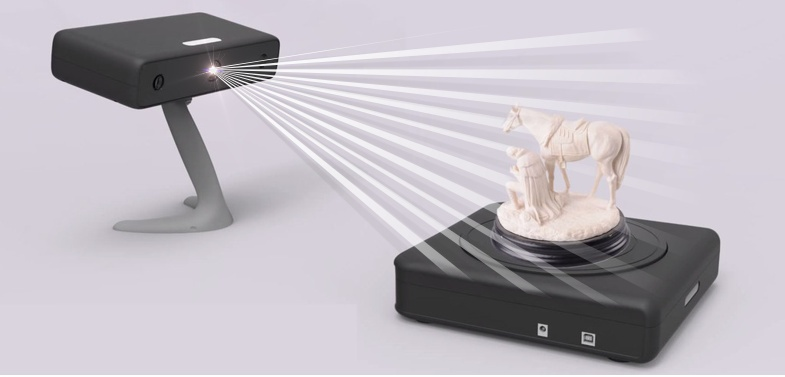
\includegraphics[scale=0.6]{figuras/scan3d.jpg}
\caption{Aquisição de modelo do mundo real por scanner 3D.}
\Fonte{www.3dprintingsystems.com}
\label{fig:scan3d}
\end{figure}

No entanto, otimizar uma malha com ruídos preservando as suas características geométricas não é uma tarefa simples. Efeitos colaterais podem ocorrer, como perda de características e retração ou expansão de volume. Para superar esses desafios, muitas técnicas de otimização de malhas foram propostas nos últimos anos. Essas técnicas fazem parte de uma área chamada Processamento de Geometria, também conhecida como Processamento de Malha, que utiliza conceitos da matemática aplicada, ciência da computação e engenharia para desenvolver algoritmos eficientes para aquisição, reconstrução, análise, manipulação, simulação e transmissão de modelos 3D complexos. Aplicações de algoritmos de processamento de malha cobrem desde áreas de multimídia, entretenimento, CAD, à computação biomédica e científica e engenharia reversa. O nome sugere uma analogia ao processamento de sinais e processamento de imagem. Muitos conceitos, estruturas de dados e algoritmos são diretamente análogos. A técnica de otimização de malha apresentada nesta dissertação se baseia diretamente nos conceitos apresentados em suavização de imagens.

De forma geral, o processamento de geometria trabalha com modelos, geralmente 2D ou 3D, baseados em malha (Figura \ref{fig:mshvsnonmsh}). Processar um modelo envolve três estágios: aquisição, tratamento e finalização. Um modelo pode ser criado por programas de modelagem, representações matemáticas ou scanner. Depois que o modelo é adquirido, ele passa por um processo de otimização, onde todas as falhas e ruídos (Figura \ref{fig:noisymodels}) serão tratados e eliminados. Finalmente, na última fase do processamento, o modelo pode ser utilizado como produto (impressoras 3D) ou em algum outro programa.

\section{Objetivos e Contribuições}

O principal objetivo deste trabalho é apresentar uma técnica de otimização de malhas de filtragem bilateral com um passo de pré-processamento. A técnica proposta visa otimizar, principalmente, malhas que possuem regiões com elementos de baixa qualidade. Entretanto, o método apresentado otimiza com sucesso qualquer tipo de malha com ruído. A técnica foi projetada para atender aos seguintes propósitos:

\begin{itemize}  
\item Detectar regiões com elementos de baixa qualidade que possam atrapalhar a otimização da malha e, então, gerar melhores elementos nessas regiões;
\item Suavizar e remover com sucesso ruídos da malha;
\item Manter, ao máximo, todas as características, detalhes e volume da malha.
\end{itemize}


\begin{figure}[!t]
\captionsetup{width=16cm}
\centering
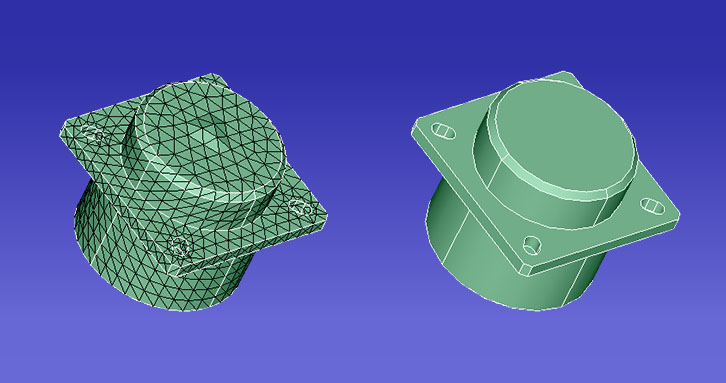
\includegraphics[scale=0.55]{figuras/meshvsnonmesh.jpg}
\caption{Exemplo de modelo 3D baseado em malha e baseado em superfície.}
\Fonte{www.altairhyperworks.com}
\label{fig:mshvsnonmsh}
\end{figure}



\begin{figure}[!t]
\captionsetup{width=13cm}
\centering
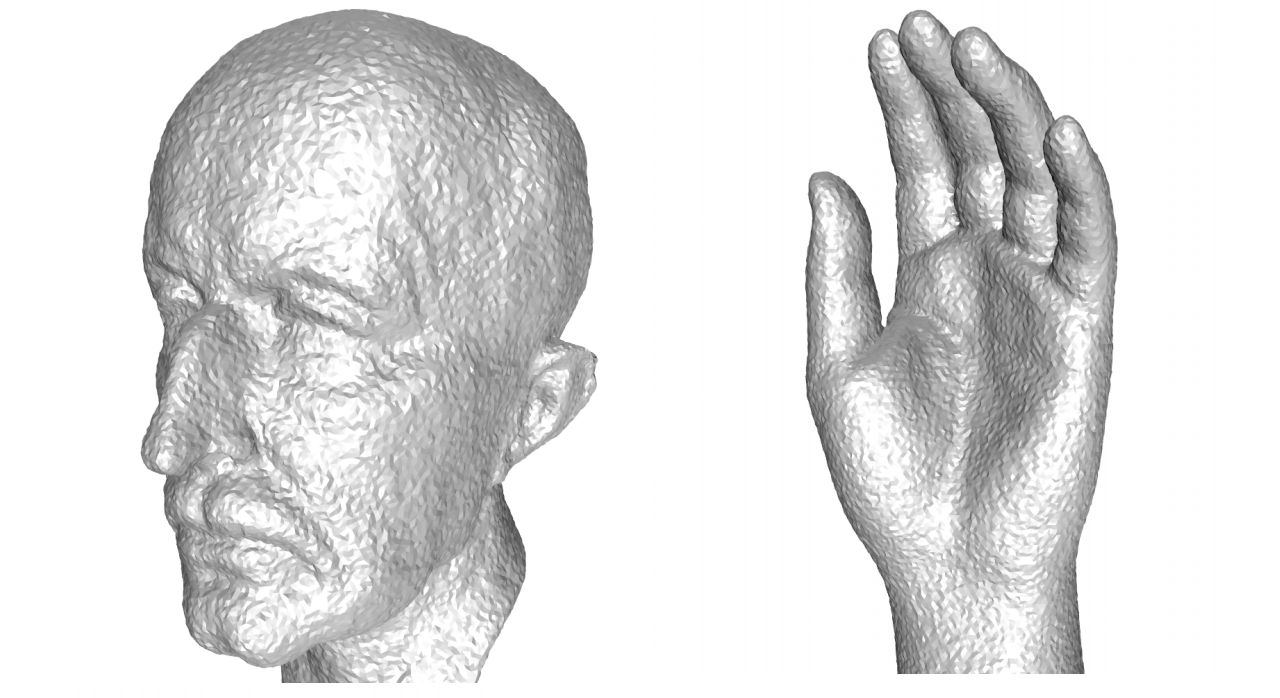
\includegraphics[scale=0.55]{figuras/noisymodels.png}
\caption{Exemplos de modelos 3D com ruídos derivados do processo de aquisição por scanner.}
\Fonte{www.altairhyperworks.com}
\label{fig:noisymodels}
\end{figure}

\section{Organização do Trabalho}
O restante deste trabalho está organizado em quatro capítulos. No Capítulo 2, apresenta-se uma visão geral das técnicas de otimização de malhas com ruídos, dividindo-as em categorias e salientando suas vantagens, desvantagens e propósitos. No Capítulo 3, é apresentada a técnica de otimização de malhas com ruído desenvolvida, detalhando todo o processo e a criação dos modelos de teste. No Capítulo 4, são apresentados os resultados da aplicação da técnica desenvolvida nos modelos de teste criados e em um modelo do mundo real, para demonstrar a sua eficácia. Os resultados obtidos são analisados por métricas para que eles sejam validados com sucesso. Por fim, no Capítulo 5, são expostas as conclusões sobre o trabalho e ideias para futuras melhorias.


	\chapter{Trabalhos Relacionados}
\label{cap:trabalhos-relacionados}

Neste capítulo, são apresentados os trabalhos relacionados na área de otimização de malhas com ruídos, mostrando as vantagens e desvantagens de cada técnica apresentada. Eles podem ser divididas basicamente em duas categorias: técnicas \textit{isotrópicas} e \textit{anisotrópicas}. Métodos isotrópicos são mais simples e só consideram informações intrínsecas ao modelo, enquanto métodos anisotrópicos, dentre os quais a técnica proposta se enquadra, usam outras informações, não inerentes diretamente ao modelo, para decidir como a filtragem deve ocorrer.

\section{Métodos isotrópicos}
O mais simples, e de melhor custo-benefício, método isotrópico é a suavização \textit{Laplaciana} (Figura \ref{fig:laplacian}), que move, iterativamente, todos os vértices do modelo em direção ao centro dos seus vizinhos, definindo, para cada vértice, a seguinte equação:
\begin{equation} \label{eq:laplacian}
    x_i = \frac{1}{N} \sum^{N}_{j=1} x_j,
\end{equation}
onde $N$ representa a quantidade de vértices adjacentes ao vértice de índice $i$, $x_j$ é a posição do vértice de índice $j$ adjacente ao vértice de índice $i$, e $x_i$ é a nova posição do vértice de índice $i$.

\begin{figure}[!h]
\captionsetup{width=\linewidth}
\centering
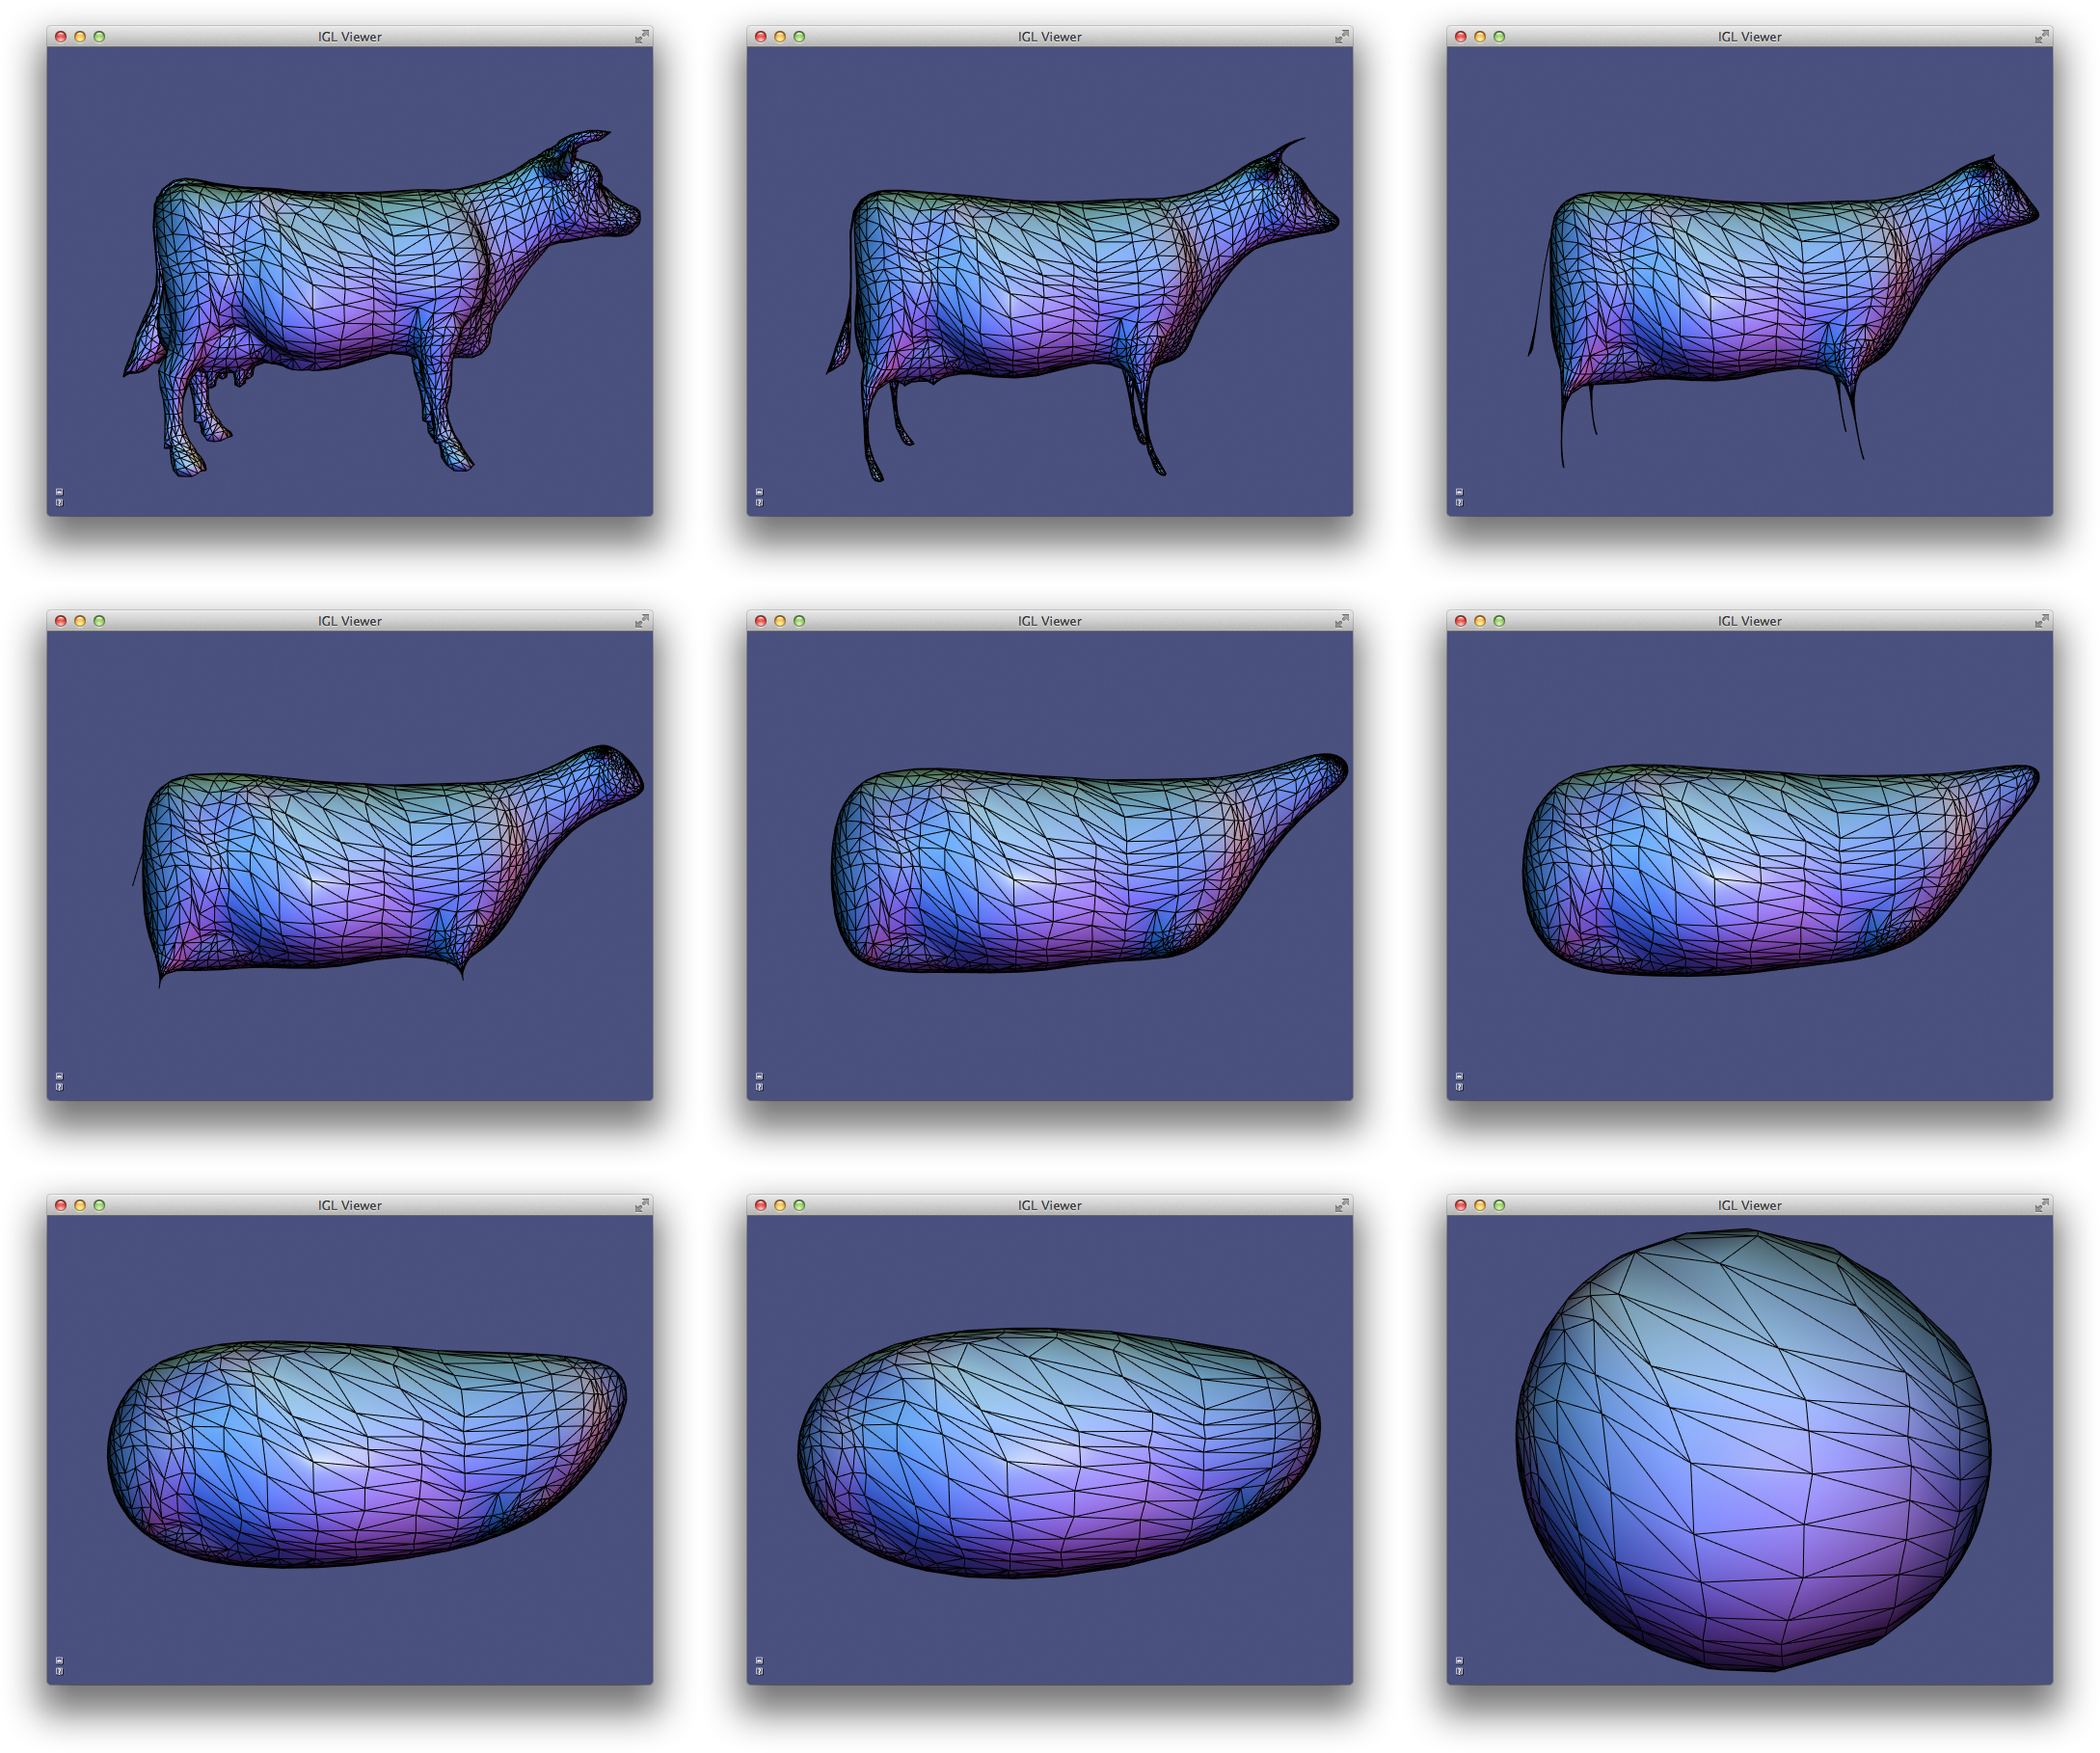
\includegraphics[scale=0.12]{figuras/laplacian.jpg}
\caption{Laplaciano aplicado ao modelo \textit{cow}. Redução de volume e perda de características podem ser notadas ao longo da aplicação do operador.}
\Fonte{http://libigl.github.io/}
\label{fig:laplacian}
\end{figure}

Apesar desta técnica ser muito rápida e simples, ela pode causar redução ou ampliação de volume e perda de características da malha, caso aplicada seguidas vezes, tornando-a não recomendável em um problema real.


Algumas melhorias foram apresentadas em \cite{vollmer1999improved} tentando resolver o problema da redução do volume ao aplicar uma operação de mover o vértice à sua posição original, depois de cada iteração. O vértice modificado $\mathbf{p}_i$ (produzido pelo \textit{Laplaciano}) é movido em direção ao vértice $\mathbf{q}_i$ e (ou) em direção ao vértice original $\mathbf{o}_i$ pela média das diferenças:
\begin{equation} \label{eq:drag-back}
    \mathbf{d}_i = -(\beta \mathbf{b}_i + \frac{1 - \beta}{|Adj(i)|} \sum_{j \in Adj(i)}{\mathbf{b}_j}),
\end{equation}
onde $\beta \in [0,1]$ é um escalar que define a influência do vértice central e seus vizinhos, $Adj(i)$ é o conjunto de vértices na vizinhança de $\mathbf{q}_i$ e $\mathbf{b}_i = \mathbf{p}_i - (\alpha \mathbf{o}_i + (1 - \alpha)\mathbf{q}_i)$, onde $\alpha \in [0,1]$ define a influência do vértice anterior $\mathbf{q}_i$ e do vértice original $\mathbf{o}_i$. A Figura \ref{fig:drag-back} ilustra a Equação \ref{eq:drag-back}.

\begin{figure}[!h]
\captionsetup{width=\linewidth}
\centering
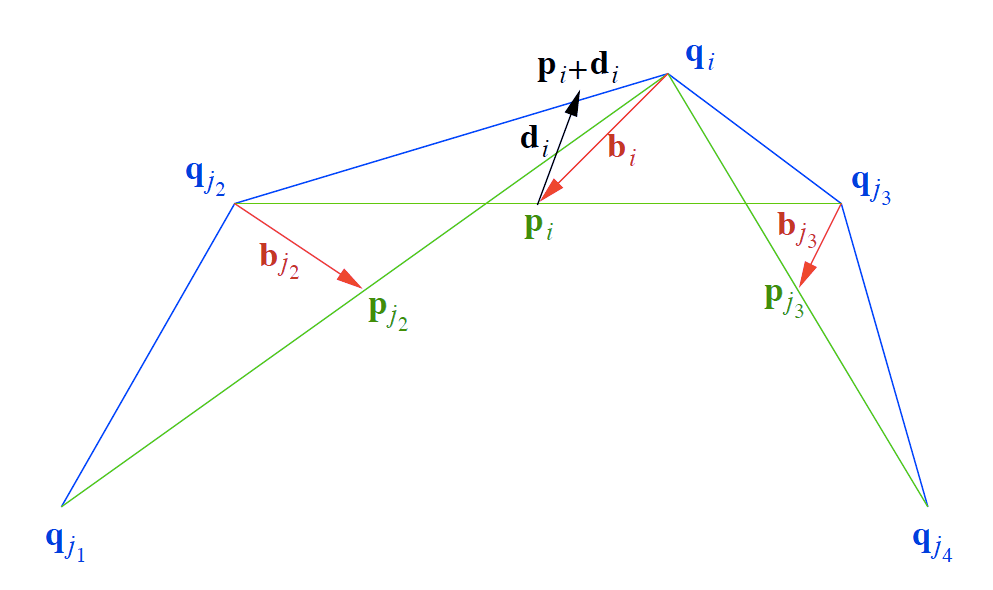
\includegraphics[scale=0.2]{figuras/drag-back-op.png}
\caption{Definição de $\mathbf{d}_i$ para mover os vértices produzidos pelo \textit{Laplaciano}. O vértice $\mathbf{o}_i$ não representado na figura, é o vértice na sua posição original antes de todas as iterações do Laplaciano.}
\Fonte{\cite{vollmer1999improved}}
\label{fig:drag-back}
\end{figure}

Esta técnica simples consegue resolver o problema da redução do volume encontrada no algoritmo de \textit{Laplace} (Figura \ref{fig:vollmerExample}) e possui algumas vantagens:
\begin{itemize}
    \item pode produzir malhas com mesmo grau de suavização do algoritmo de \textit{Laplace};
    \item preserva forma e volume da malha;
    \item rápida e de fácil implementação.
\end{itemize}

Porém, só apresenta bons resultados para modelos mais simples. Por ser uma técnica antiga, modelos mais complexos, como encontramos atualmente, não são contemplados.

\begin{figure}[!h]
\captionsetup{width=\linewidth}
\centering
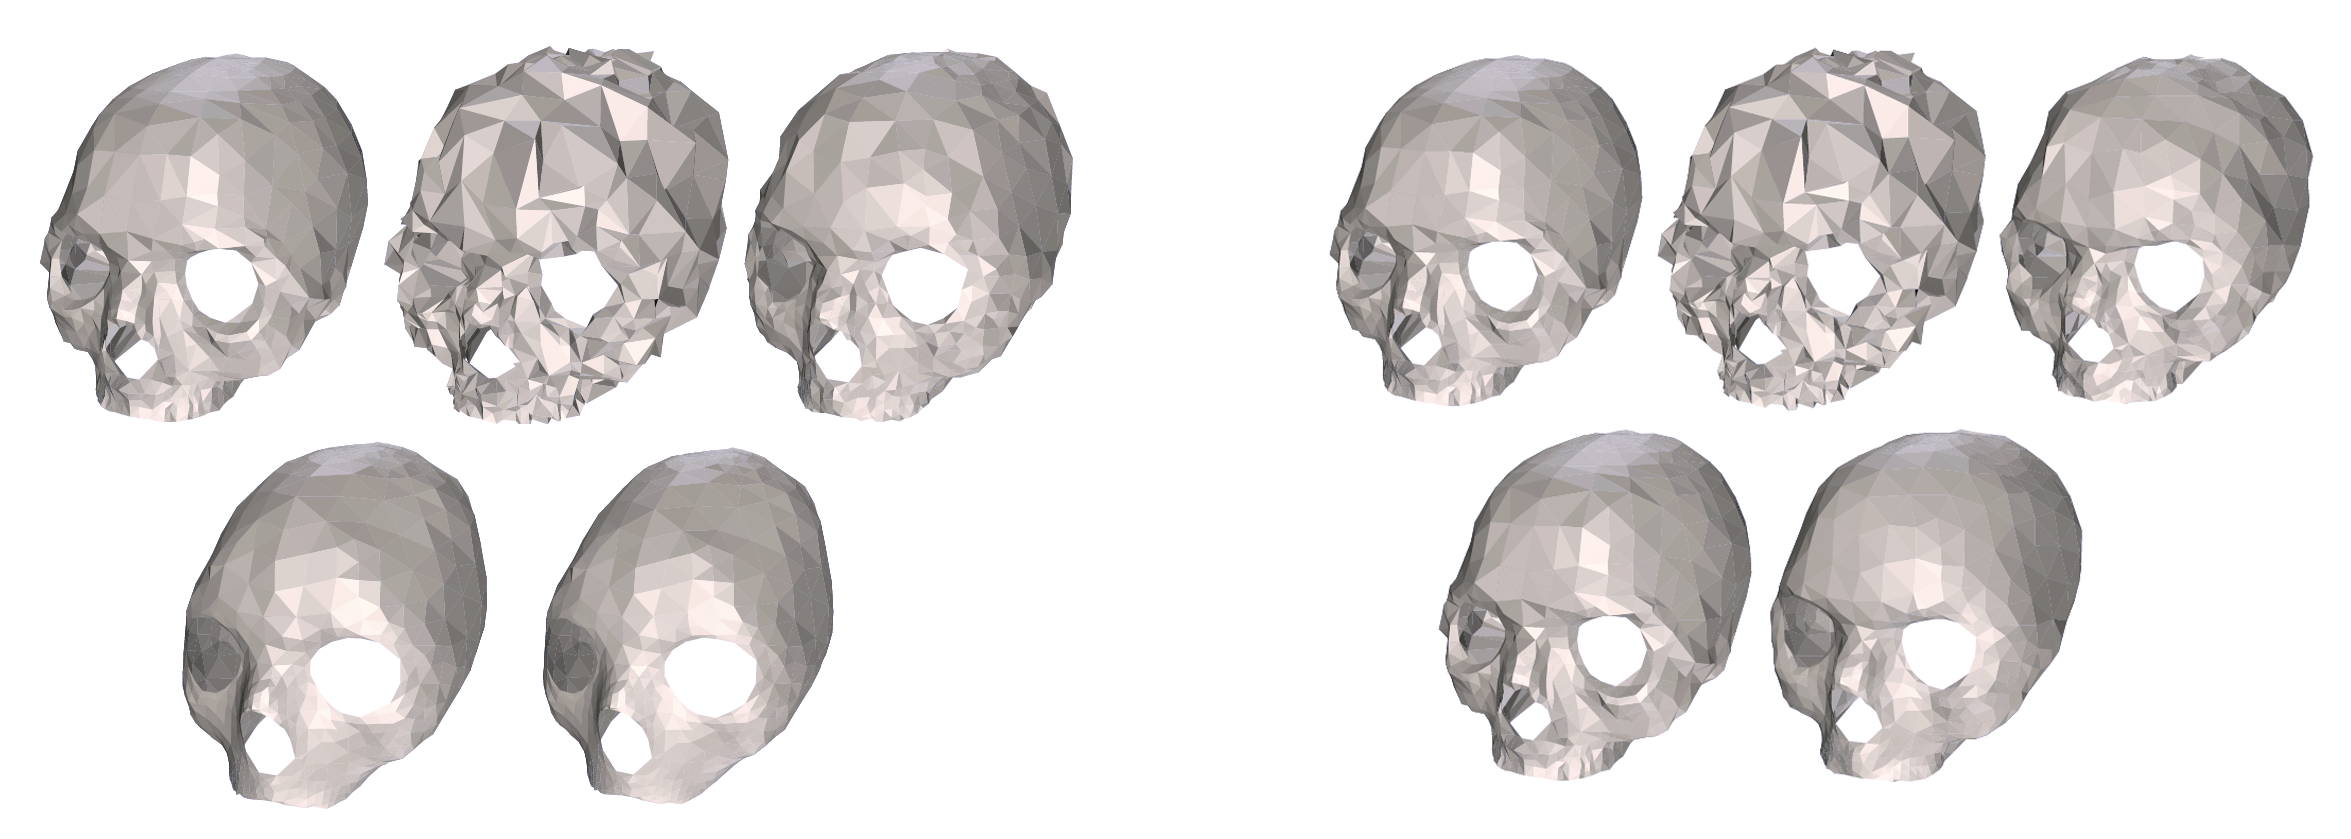
\includegraphics[width=\linewidth]{figuras/volmmerExample.png}
\caption{Esquerda: malha original, malha com ruído, 3 iterações de Laplace. Direita: malha original, malha com ruído, 3 iterações da técnica apresentada em \cite{vollmer1999improved}.}
\Fonte{\cite{vollmer1999improved}}
\label{fig:vollmerExample}
\end{figure}

Em \cite{liu2007non} um operador de otimização global é apresentado para malhas arbitrárias. Este operador global é composto de dois termos principais: operador Laplaciano global e condições de restrição para manter a fidelidade da malha. 

O operador Laplaciano, também conhecido como cordenadas diferenciais, pode ser aproximado em cada vértice pelo operador \textit{umbrella} (Figura \ref{fig:umbrella}):
\begin{equation}
    L(\mathbf{v}_i) = \sum_{j\in i^*}{w_{ij}(\mathbf{v}_j - \mathbf{v}_i}),
\end{equation}
onde $i^*$ é o conjunto de índices dos vértices vizinhos de $\mathbf{v}_i$, e $w_{ij}$ é o peso da aresta $(i,j)$ correspondendo ao vértice $\mathbf{v}_i$ com $\sum_{j\in i^*}{w_{ij} = 1}.$

\begin{figure}[!h]
\captionsetup{width=\linewidth}
\centering
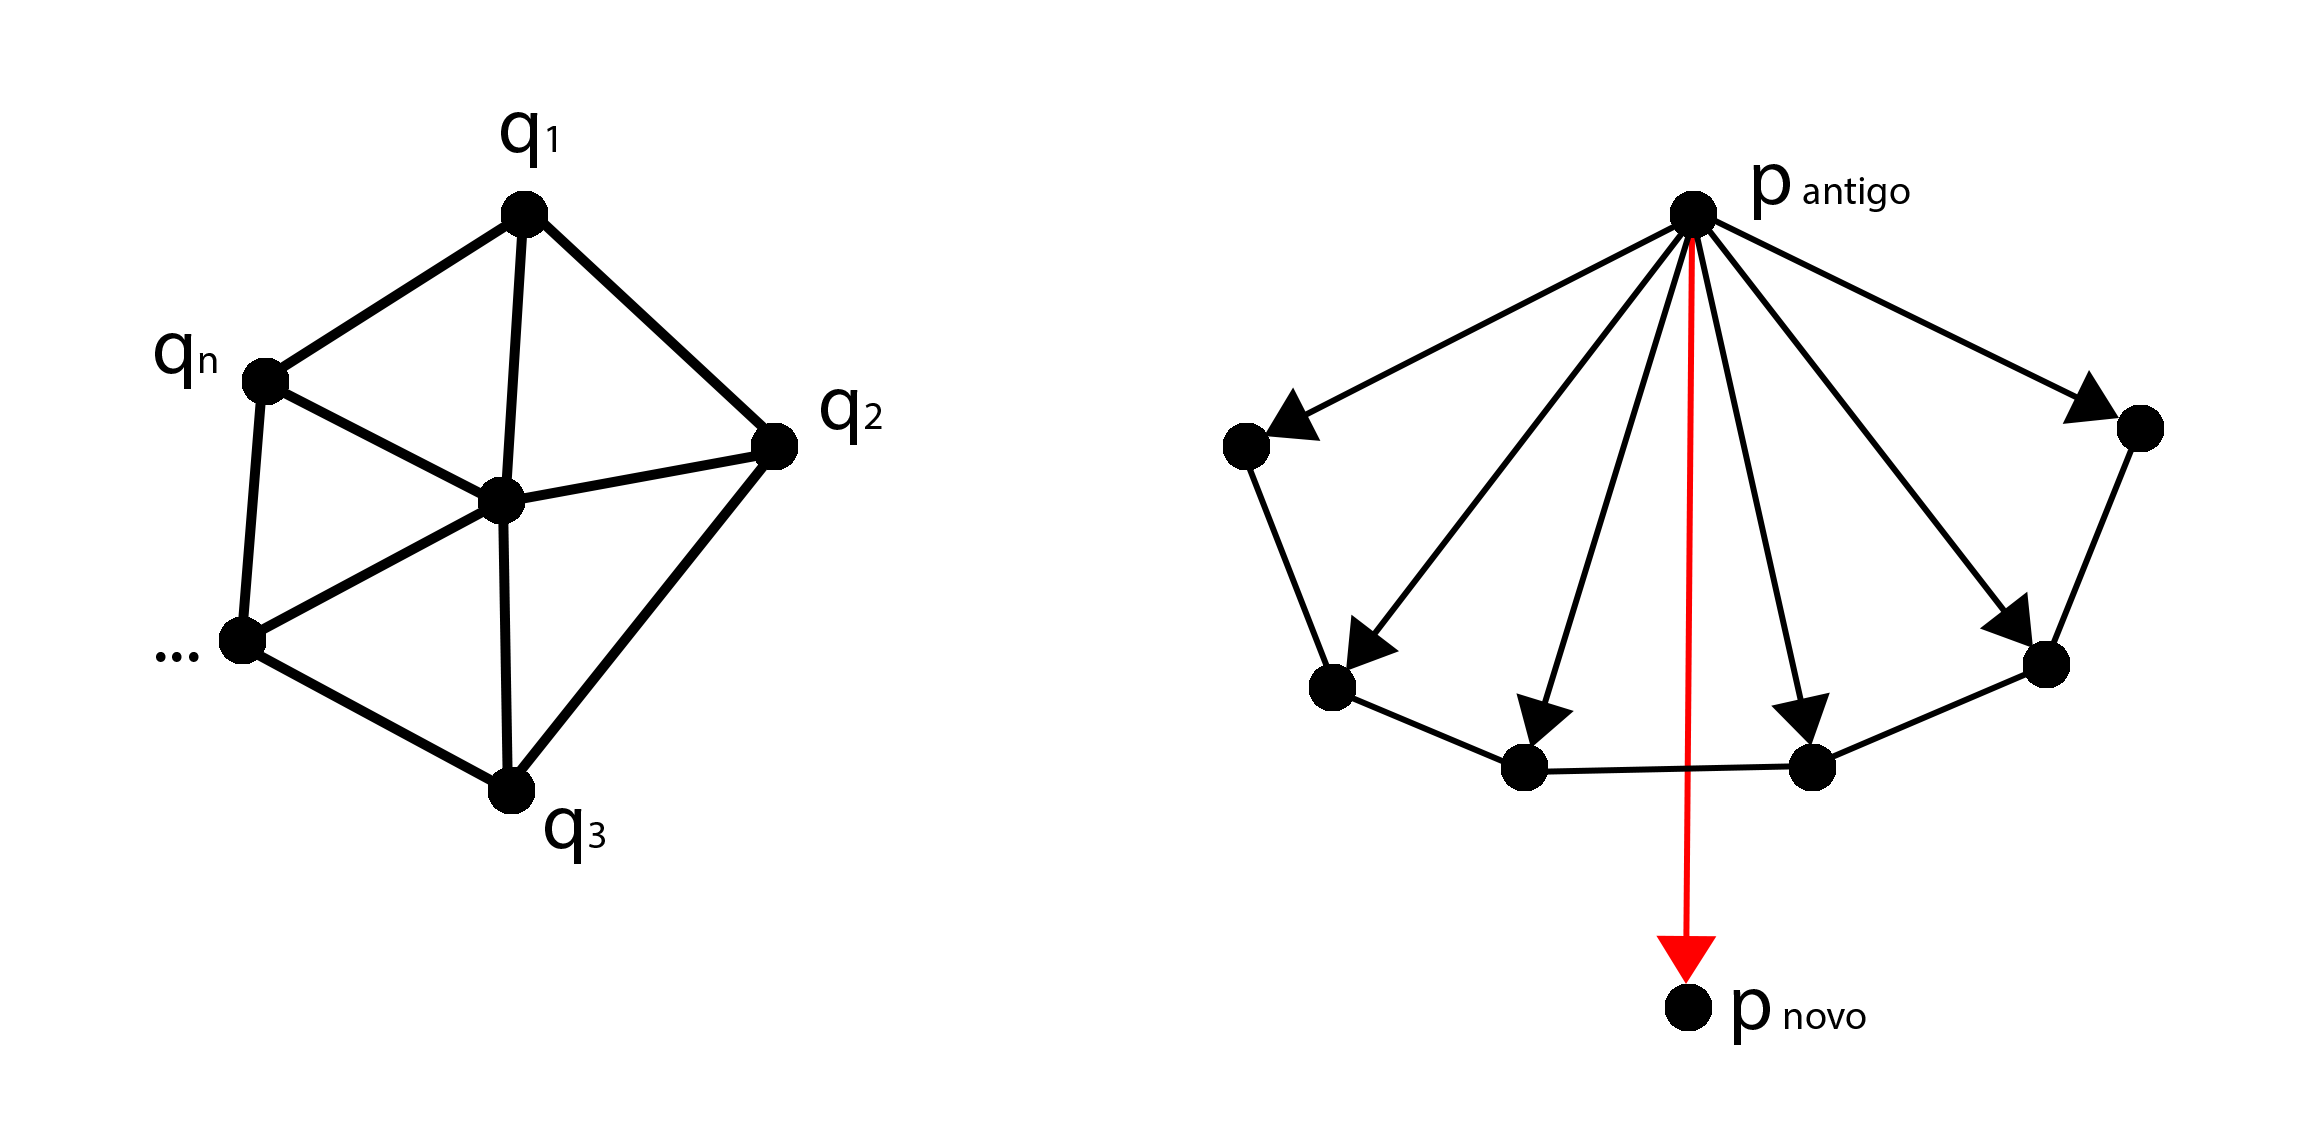
\includegraphics[scale=0.30]{figuras/umbrella_operator.png}
\caption{Definição do operador \textit{umbrella}. O ponto $p$ será movido pela média ponderada dos seus vizinhos $q_1$,.., $q_n$.}
\label{fig:umbrella}
\end{figure}

Foi observado que o vértice $\mathbf{v}_i$ permanece na média ponderada dos seus vizinhos imediatos (\textit{1-ring}) se a seguinte equação for satisfeita:
\begin{equation}
    \mathbf{v}_i - \sum_{j\in i^*}{w_{ij}\mathbf{v}_j} = 0,
\end{equation}
portanto, isto também é considerado na criação do Laplaciano global. As condições de otimização global para todos os vértices é definida da seguinte forma:
\begin{equation}
    \mathbf{L}\mathbf{X} = 0,
\end{equation}
onde $\mathbf{L}$ é uma matriz $n$ x $n$ com elementos derivados de $w_{ij}$:
\begin{equation}
L_{ij}=\left\{
\begin{array}{c l}	
     1, & i=j,\\
     -w_{ij} & (i,j) \in E, \\
     0 & c.c,
\end{array}\right.
\end{equation}
onde $X$ é o vetor coluna dos vértices correspondentes e $E$ é o conjunto de arestas da malha. Formando, dessa forma, toda a restrição de otimização do Laplaciano global.

Restrições de vértices (Figura \ref{fig:restricao_vertices}) e restrições de baricentro das faces também são aplicadas para manter características da malha. Esses vértices são detectados automaticamente ou com a ajuda do usuário.

\begin{figure}[!h]
\captionsetup{width=\linewidth}
\centering
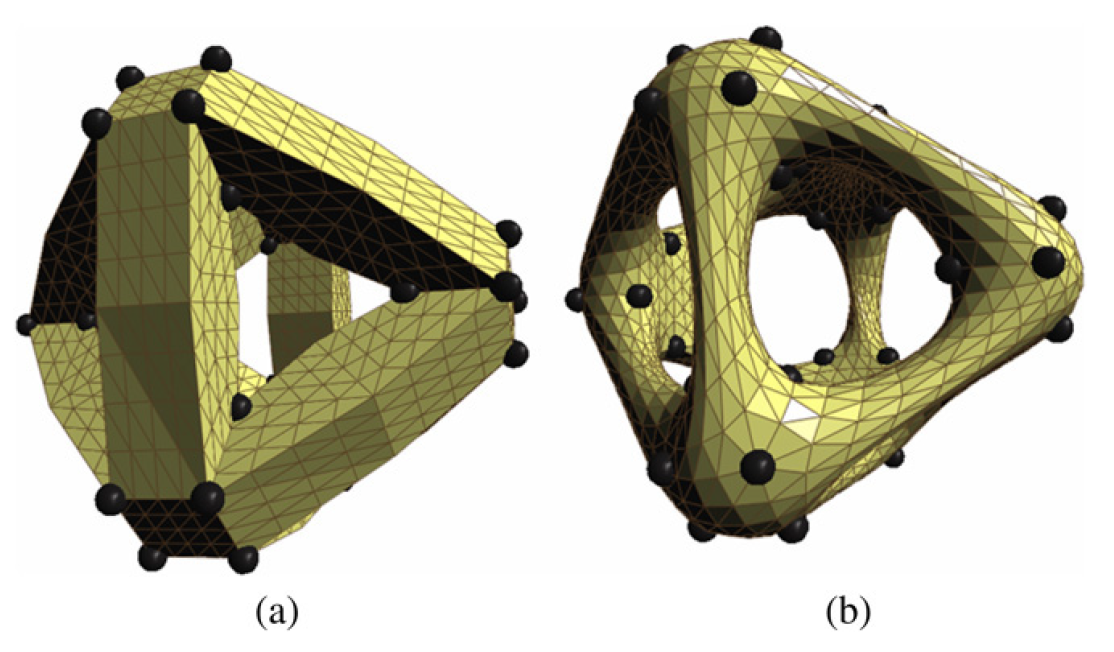
\includegraphics[scale=0.25]{figuras/restricao_vertices.png}
\caption{Otimização Laplaciana global com restrição de vértices. Os vértices da restrição estão na cor preta em destaque: (a) malha original; (b) malha otimizada.}
\Fonte{\cite{liu2007non}}
\label{fig:restricao_vertices}
\end{figure}

Apesar de resultados relevantes (Figura \ref{fig:dragon_laplaciano_global}) e da grande contribuição dos métodos isotrópicos para a área de otimização de malhas, métodos baseados no Laplaciano geralmente não conseguem preservar características e volume da malha, enquanto remove os ruídos existentes.

\clearpage

\begin{figure}[!h]
\captionsetup{width=\linewidth}
\centering
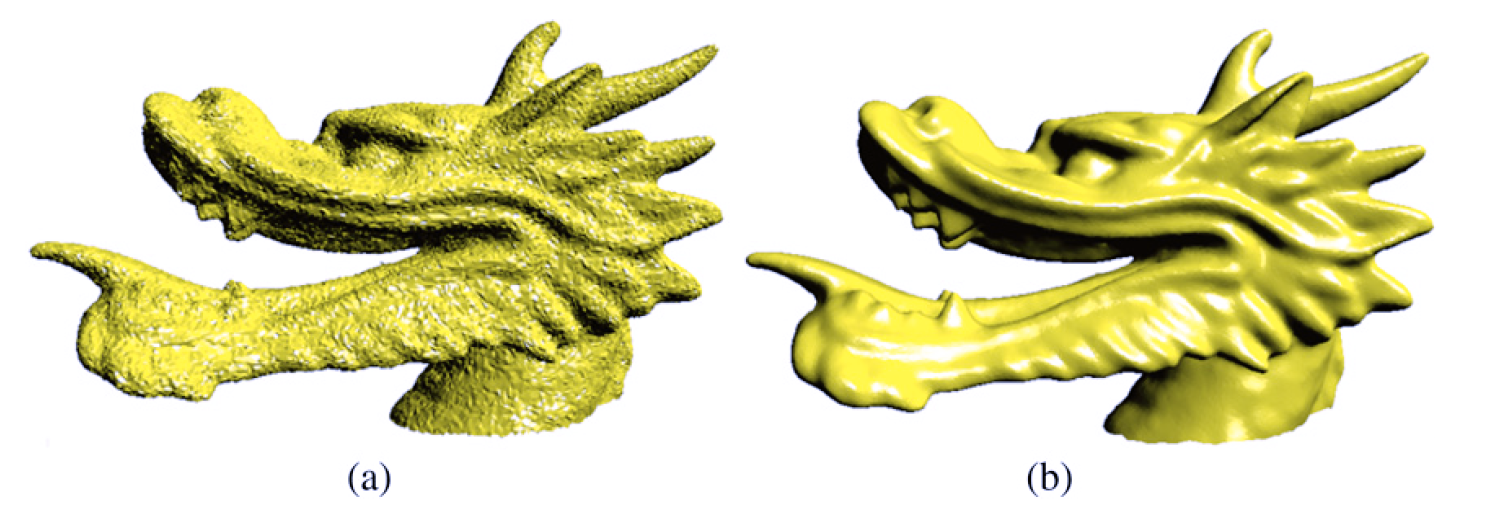
\includegraphics[scale=0.28]{figuras/dragon_laplaciano_global.png}
\caption{Resultado do uso da técnica de \cite{liu2007non}, no modelo \textit{dragon}, para remoção de ruídos: (a) o modelo \textit{dragon} com ruído; (b) o modelo \textit{dragon} otimizado com restrições de vértices e baricentro de faces.}
\Fonte{\cite{liu2007non}}
\label{fig:dragon_laplaciano_global}
\end{figure}


\section{Métodos anisotrópicos}

Neste mesmo contexto, uma variedade de métodos anisotrópicos foram criados no intuito de uma melhor preservação das características geométricas do modelo. Alguns deles se inspiraram nos conceitos propostos em processamento de imagens, como a filtragem bilateral \cite{tomasi1998bilateral}, que é, essencialmente, um filtro não-linear, para suavização de imagens, que preserva características importantes, tais como as arestas. Esta técnica substitui o valor de intensidade de um pixel pela média ponderada dos valores de intensidade dos pixels próximos. Desta forma, um pixel só é influenciado por pixels próximos com intensidade similares. A filtragem bilateral para uma imagem $I(\mathbf{u})$, em uma coordenada $\mathbf{u} = (x,y)$ é definida em \cite{tomasi1998bilateral} como:
\begin{equation}\label{eq:filtro_bilateral} 
    \hat{\mathrm{I}}(\mathbf{u}) = \frac{\sum_{p \in N(\mathbf{u})}{W_c(\|\mathbf{p}-\mathbf{u}\|)W_s(|I(\mathbf{u})-I(\mathbf{p})|)I(\mathbf{p})}}{ \sum_{p \in N(\mathbf{u})}{W_c(\|\mathbf{p}-\mathbf{u}\|)W_s(|I(\mathbf{u})-I(\mathbf{p})|)} },
\end{equation}
onde $N(\mathbf{u})$ é a vizinhança de pixels de $\mathbf{u}$, $W_c(x) = e^{-x^2/2\sigma_c^2}$, com parâmetro $\sigma_c$, representa o kernel Gaussiano de proximidade e $W_s(x) = e^{-x^2/2\sigma_s^2}$, com parâmetro $\sigma_s$, representa o kernel de intensidade.

O sucesso dessa abordagem em processamento de imagens levou à sua adaptação na área de processamento de geometria, em técnicas de remoção de ruído e suavização de malhas \cite{fleishman2003bilateral, jones2003non, zheng2011bilateral, solomon2014general}.

Em \cite{fleishman2003bilateral}, os vértices são filtrados na direção da normal usando-se os seus vizinhos locais. A técnica parte do pressuposto de que todo vértice $v$ na malha com ruído está a uma distância $d_v$ para a malha \textit{ground-truth}, que é a malha completamente sem ruído utilizada para comparação do resultado da otimização da malha com ruído. Portanto essa distância é estimada aplicando o filtro iterativamente, atualizando $v$ da seguinte forma:
\begin{equation}
    v = v + d \cdot n,
\end{equation}
onde $n$ é o vetor normal associado a $v$, que irá direcionar o deslocamento de $v$. O filtro é aplicado a cada vértice, calculando o seu deslocamento e atualizando sua posição baseada na Equação \ref{eq:filtro_bilateral}.

Em \cite{jones2003non}, uma técnica de filtragem bilateral de malhas com ruídos, baseada em estimativas estatísticas robustas, é apresentada. O modelo se baseia na afirmação de que uma técnica de suavização, que preserva as características da malha, pode ser vista meramente como um problema de estimar uma superfície na presença de \textit{outliers}. A extensão de métodos estatísticos robustos para técnicas de filtragem de superfície não é algo trivial. Para a obtenção da suavidade de uma superfície, são definidos preditores locais de primeira ordem (Figura \ref{fig:predictions}). Com um estimador robusto, são achadas as novas posições de cada vértice como uma soma ponderada das predições na sua vizinhança espacial.


\begin{figure}[!h]
\captionsetup{width=\linewidth}
\centering
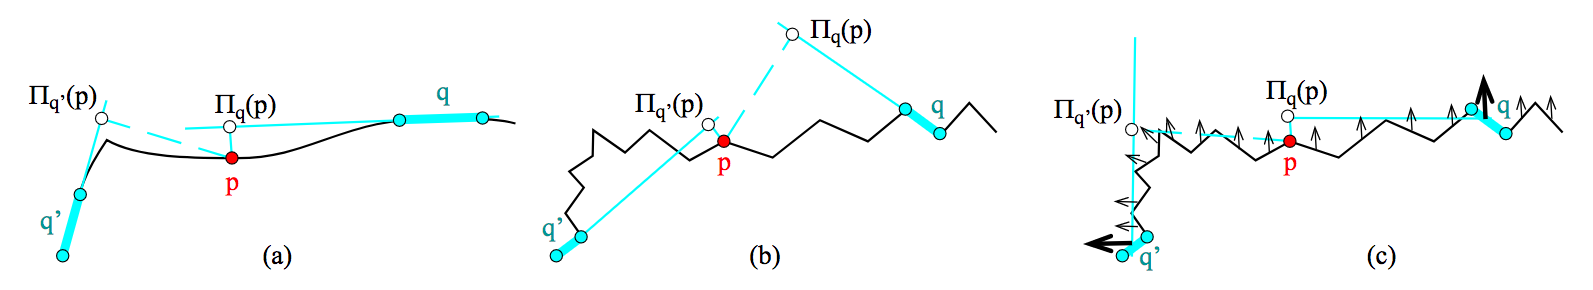
\includegraphics[scale=0.28]{figuras/predictions.png}
\caption{(a) A predição $\Pi_q(p)$ para um ponto $p$, baseado na superfície de $q$, é a projeção de $p$ no plano tangente formado pela superfície de $q$. Pontos em regiões de linhas características (arestas) resultam em predições mais distantes e, portanto, causando menos influência. (b) Normais com ruídos podem levar a más predições. (c) Normais melhoradas mitigam este problema, pois os planos tangentes são construídos baseados nelas. }
\Fonte{\cite{jones2003non}}
\label{fig:predictions}
\end{figure}

Apesar de apresentar bons resultados, e mostrar que a filtragem bilateral é robusta a \textit{outliers}, esse método depende, fortemente, da aproximação dos preditores locais, e estes são muito sensíveis a ruídos, mesmo com o passo de melhoria das normais. 

A eficácia da filtragem bilateral foi estendida pela filtragem bilateral conjunta (\textit{joint}) em \cite{eisemann2004flash}, \cite{petschnigg2004digital}. A ideia é que os pesos associados podem ser determinados usando as diferenças de intensidades de uma outra imagem, chamada \textbf{guia} (Figura \ref{fig:flash-noflash}). A filtragem bilateral conjunta atinge melhores resultados que a filtragem bilateral clássica, quando a imagem guia proporciona melhores informações do que a imagem de entrada a ser tratada. A filtragem bilateral conjunta foi usada com sucesso em processamento de imagens, conseguindo bons resultados. O verdadeiro desafio é a sua adaptação aos sinais geométricos, para que possa ser usado, também, em técnicas de otimização de malhas. Diferentemente dos sinais definidos nas imagens (e.g valor de intensidade em um pixel), que estão limitados a domínios simples e retangulares, os sinais geométricos (e.g posição de um vértice, normais, planos tangentes etc) são, geralmente, definidos em relação à superfície da malha, que possui topologia arbitrária e amostragem de elementos irregular. Esse guia geométrico tem que ser, comumente, construído computacionalmente.

\begin{figure}[!h]
\captionsetup{width=\linewidth}
\centering
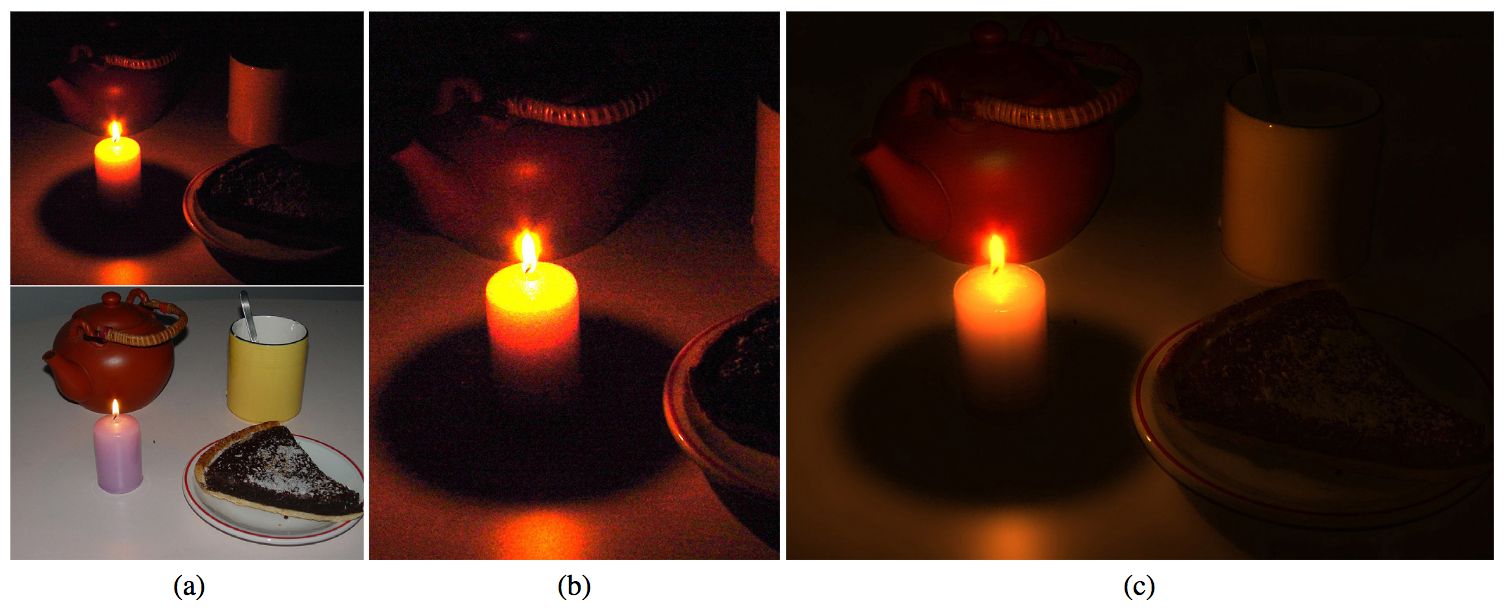
\includegraphics[scale=0.3]{figuras/flash-noflash.png}
\caption{(a) Cima: Fotografia tirada em um ambiente escuro, a imagem possui ruído e embaçamento. Baixo: Mesma fotografia com flash, provendo uma imagem com maiores detalhes, porém plana e possuindo sombras indesejadas na silhueta dos objetos. (b) Ampliação da imagem mostrando o ruído presente. (c) Técnica de \cite{eisemann2004flash} misturando as duas imagens (com flash e sem flash) para transferir a luz do ambiente à imagem principal.}
\Fonte{\cite{eisemann2004flash}}
\label{fig:flash-noflash}
\end{figure}

Em \cite{zheng2011bilateral} também é apresentada uma técnica baseada no filtro bilateral de \cite{tomasi1998bilateral} e o filtro bilateral conjunto de \cite{eisemann2004flash} e \cite{petschnigg2004digital}. São apresentados dois esquemas de remoção de ruídos. Além da abordagem de aplicar o filtro bilateral nas normais da malha com uma formulação iterativa e local (apenas considerando a intensidade das normais na vizinhança), é apresentado, também, uma formulação, não iterativa, global para remoção de ruídos em malhas. É mostrado que a formulação global é mais robusta para malhas com ruídos possuindo triangulações irregulares, enquanto que a formulação local recupera mais rapidamente, e mais efetivamente, malhas com uma maior quantidade e intensidade de ruídos (Figura \ref{fig:globalxlocal}).

\begin{figure}[!h]
\captionsetup{width=\linewidth}
\centering
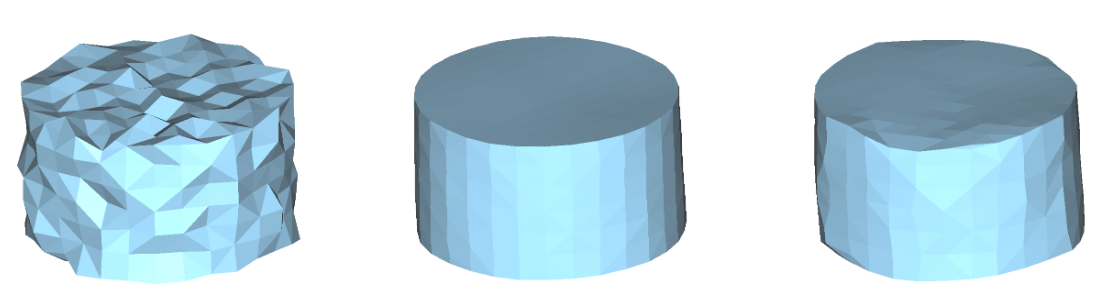
\includegraphics[scale=0.3]{figuras/globalxlocal.png}
\caption{Remoção de ruídos do modelo cilíndro (a esquerda). A formulação local (meio) recupera, mais eficientemente, as características geométricas do que a formulação global (direita) quando o nível de ruído é elevado.}
\Fonte{\cite{zheng2011bilateral}}
\label{fig:globalxlocal}
\end{figure}

Em \cite{solomon2014general}, uma generalização do filtro bilateral é apresentada. Um \textit{framework} que pode ser usado para suavizar sinais definidos em imagens, malhas e outros domínios. A construção da técnica é reduzida, exatamente, ao filtro bilateral para imagens em domínios retangulares. É mostrado também a aplicação do \textit{framework} a outros efeitos geométricos como o aprimoramento de características. A principal contribuição da técnica é a maior customização dos \textit{kernels} definidos no filtro bilateral (Figura \ref{fig:kernelframework}), fazendo com que seja possível aplicar a técnica de uma forma generalizada e em várias aplicações.

\begin{figure}[!h]
\captionsetup{width=\linewidth}
\centering
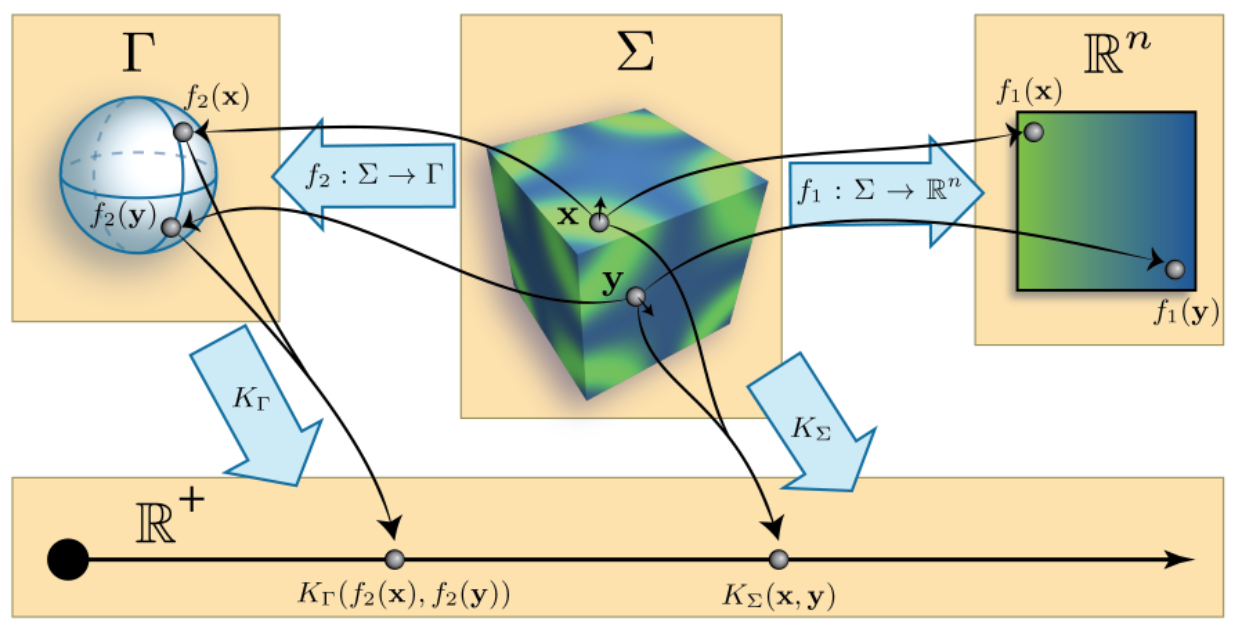
\includegraphics[scale=0.3]{figuras/kernelframework.png}
\caption{\textit{Kernels} $f_1$ e $f_2$ definidos em relação a uma esfera e a uma textura, respectivamente.}
\Fonte{\cite{solomon2014general}}
\label{fig:kernelframework}
\end{figure}

Em suma, \cite{fleishman2003bilateral} e \cite{jones2003non} usam a filtragem bilateral simples, aplicando o filtro diretamente nos vértices da malha, enquanto \cite{zheng2011bilateral} e \cite{solomon2014general} aplicam a filtragem bilateral conjunta nas normais das faces, seguido de uma atualização nas posições dos vértices baseada nas normais filtradas. A dificuldade encontrada nesse processo advém da natureza das normais encontradas em modelos com ruídos, que geralmente estão corrompidas pelo próprio ruído da malha, não sendo um bom guia para a filtragem bilateral conjunta, levando assim a resultados insatisfatórios.

Em \cite{zhang2015guided}, é mostrado como calcular um campo de normais guia mais confiável e robusto para a filtragem bilateral conjunta de malhas com ruídos. As novas normais guias serão computadas a partir da média das normais das faces vizinhas, e essas novas normais irão guiar a atualização dos vértices da malha (no trabalho proposto nessa dissertação, a mesma construção do campo de normais guia será utilizada, portanto mais detalhes sobre este processo serão descritos no Capítulo \ref{chap:tecnicaproposta}). A abordagem de usar a filtragem bilateral conjunta nas normais das faces e atualizar as posições dos vértices a partir dessas normais também foi adotada por muitos outros trabalhos \cite{sun2007fast, yagou2002mesh, chen2005sharpness, sun2008random}, diferindo entre eles na estratégia de filtragem das normais. Todos esses métodos anisotrópicos são focados principalmente em preservar características do modelo no processo de remoção de ruído, demonstrando pouca atenção na melhoria da qualidade da malha. Afim de otimizar uma malha com ruído enquanto melhora sua regularidade, \cite{wei2013feature} apresentam um método de dois passos que usa a filtragem bilateral conjunta juntamente com a suavização Laplaciana com restrições (Figura \ref{fig:filtroEregularidade}). 

\begin{figure}[!h]
\captionsetup{width=\linewidth}
\centering
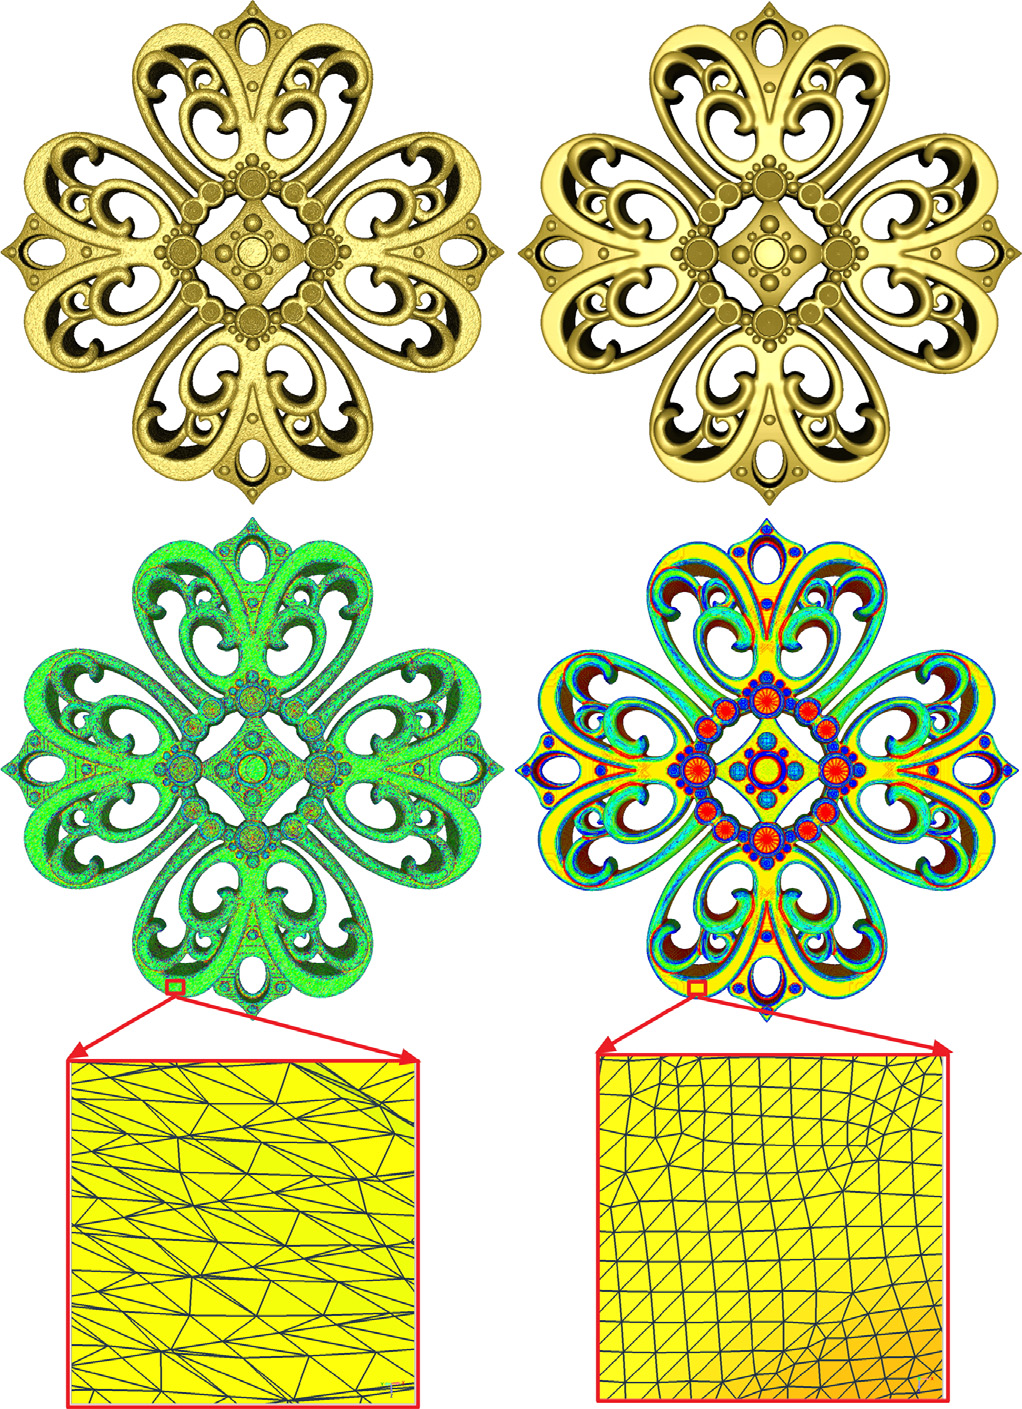
\includegraphics[scale=0.2]{figuras/filtroEregularidade.png}
\caption{Otimização do modelo \textit{Filgree} usando a técnica proposta em \cite{wei2013feature}. A primeira linha mostra a geometria do modelo com ruído (esquerda) e do modelo otimizado (direita). A linha do meio ilustra a visualização da curvatura média, e a linha de baixo mostra os fragmentos ampliados.}
\Fonte{\cite{wei2013feature}}
\label{fig:filtroEregularidade}
\end{figure}

\section{Considerações Finais}

As técnicas discutidas neste capítulo apresentam bons resultados na maioria dos casos, mas falham em otimizar malhas com grande presença de ruídos ou com amostragem de faces extremamente irregular (Figura \ref{fig:irregularSampling}). Não há garantia de que modelos gerados a partir de um \textit{scanner} 3D possuam uma malha com amostragem regular de faces. Desta forma, uma técnica de otimização de modelos com ruídos pode gerar resultados indesejados.

\begin{figure}[!h]
\captionsetup{width=\linewidth}
\centering
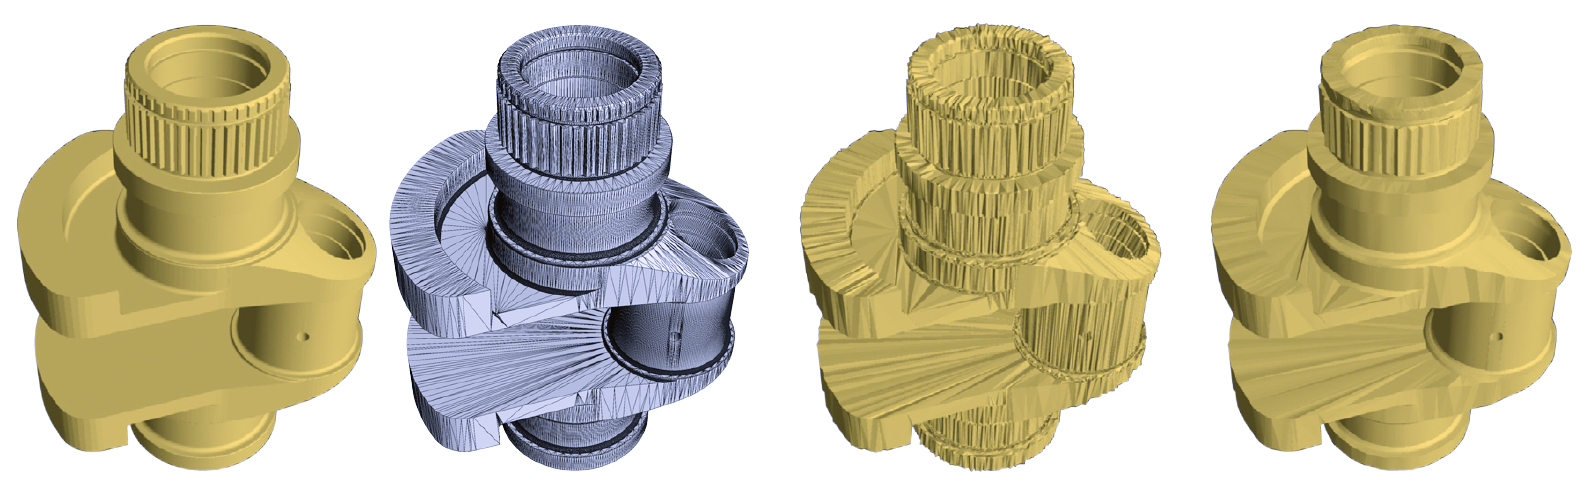
\includegraphics[width=\linewidth]{figuras/irregularSampling.png}
\caption{Da esquerda para a direita: Modelo sem ruído (\textit{ground-truth}), \textit{ground-truth} mostrando a malha associada ao modelo, modelo com ruído sintético, resultado da técnica de \cite{zhang2015guided}. }
\Fonte{\cite{zhang2015guided}}
\label{fig:irregularSampling}
\end{figure}













%\Gls{ambiguidade}
%\Gls{braile}
%\Gls{coerencia}
%\Gls{dialetos}
%\Gls{elipse}
%\Gls{locucao-adjetiva}
%\Gls{modificadores}
%\Gls{paronimos}
%\Gls{sintese}
%\Gls{borboleta}
	\chapter{Técnica proposta}
\label{chap:tecnicaproposta}

Nesse capítulo é apresentada a técnica proposta de filtragem bilateral com pré-processamento. Ela visa atender principalmente modelos com ruídos que possuem qualidade de triangulação ruim e foi projetada para atender os seguintes propósitos:

\begin{itemize}  
\item Detectar regiões com elementos de baixa qualidade que possam atrapalhar a otimização da malha e, então, gerar melhores elementos nelas;
\item Suavizar e remover com sucesso ruídos da malha;
\item Manter, ao máximo, todas as características, detalhes e volume da malha;
\end{itemize}

O primeiro ponto é muito importante visto que alguns modelos gerados por scanners ópticos, geralmente, não geram uma boa triangulação e, a maioria das técnicas de filtragem bilateral não apresenta bons resultados para este tipo de malha.

O segundo ponto trata do quesito mais importante de qualquer técnica de filtragem de malha para remoção de ruídos: apresentar uma malha resultante semelhante reduzindo quase que totalmente os ruídos da malha original.

Quanto ao terceiro ponto, embora existam técnicas mais simples e menos robustas (operador de Laplace-Beltrami ou Laplaciano) para suavização de malhas, podem-se notar perdas de características essenciais e redução ou aumento de volume na malha resultante. A filtragem bilateral de normais combate esses dois problemas de forma mais eficiente.

\section{Descrição Geral}

Na técnica proposta a entrada é uma malha $M$ com ruído. Uma análise será feita à procura de regiões (\textit{patches}) com qualidade de triangulação ruim. Todas essas regiões selecionadas serão apagadas da malha $M$ (gerando uma nova malha $M'$) e mantida em outra malha $M_p$, que será utilizada como base na reconstrução das regiões apagadas de $M'$. Um processo de reconstrução é implementado nas regiões apagadas da malha $M'$ (utilizando a malha $M_p$ como guia) gerando uma malha idêntica a $M$, porém com mais detalhes nas regiões reconstruídas, denominada $M_0$. Após a reconstrução, o filtro bilateral é executado $k$ vezes, produzindo uma malha final $M_k$ sem ruídos. A Figura \ref{fig:steps} mostra o fluxo geral da técnica proposta.

\begin{figure}[!t]
\captionsetup{width=\linewidth}
\centering
\includegraphics[width=\linewidth]{figuras/steps.png}
\caption{Fluxo geral da técnica proposta: Primeiramente é selecionado um ou mais \textit{patches} de faces de qualidade inferior às demais; em sequência esses \textit{patches} são apagados e melhores elementos são gerados em seu lugar. Como último passo, $k$ iterações são executadas intercalando o filtro bilateral nas normais das faces e a atualização da posição dos vértices baseado nessas normais filtradas.}
\label{fig:steps}
\end{figure}

\subsection{Pré-processamento}

Processos de aquisição de modelos 3D do mundo real algumas vezes não conseguem êxito na digitalização sem falhas do objeto, podendo ele ser processado com ruído e até mesmo ser gerado possuindo uma malha de elementos com qualidade insatisfatória. Como primeiro passo da técnica proposta, uma análise é feita na malha a ser processada. Este processo tem como objetivo identificar possíveis elementos que possam prejudicar o resultado final do filtro bilateral. A Figura \ref{fig:comparisonwithoutpreprocessing} exibe o resultado da aplicação da filtragem bilateral em um modelo que possui alguns elementos de qualidade ruim, mostrando assim a necessidade de um pré-processamento para que o modelo não aumente ou diminua seu volume e nem perca suas características provindas do modelo original.


\begin{figure}[!h]
\captionsetup{width=\linewidth}
\centering
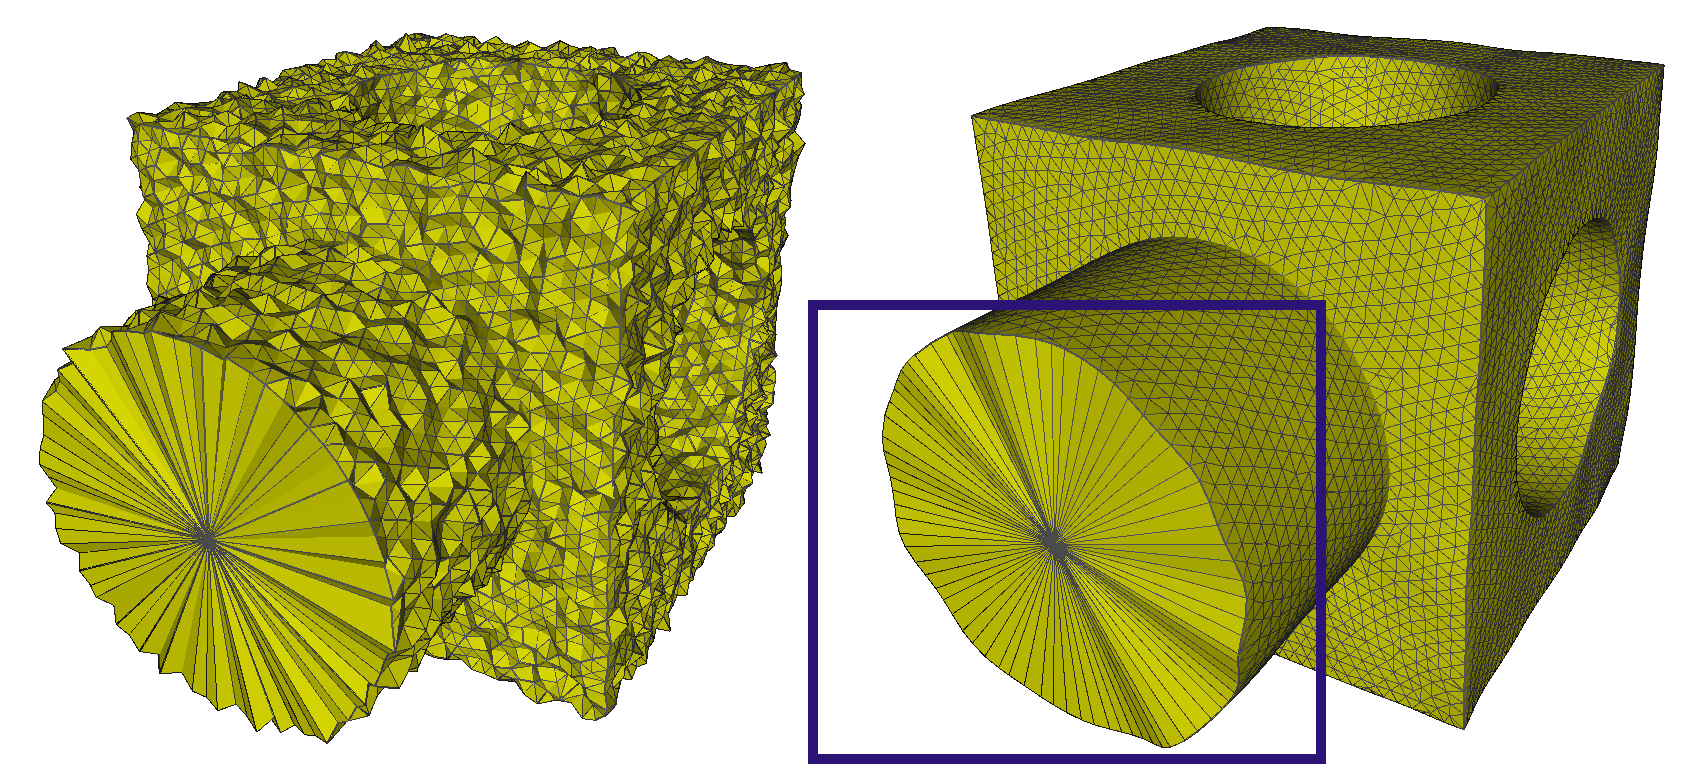
\includegraphics[width=\linewidth]{figuras/comparison.png}
\caption{Filtro bilateral sem pré-processamento aplicado ao modelo \textit{block} com ruído artificial. Na área demarcada pode-se notar perda de característica do modelo original.}
\label{fig:comparisonwithoutpreprocessing}
\end{figure}


\subsubsection{Seleção de \textit{patches}}

Seja $M = (V,E,F)$ uma malha com ruído, onde $V$, $E$ e $F$ são os conjuntos de vértices, arestas e faces, respectivamente, de $M$. Um conjunto de faces (\textit{patches}) de $M$, que pode interferir no filtro bilateral, será então selecionado, de forma manual ou automática, (Figura \ref{fig:validselection}) e extraído. Uma nova malha $M_p$ será então gerada contendo apenas os elementos deletados de $M$. No final deste processo (Figura \ref{fig:meshparts}) terão-se duas novas malhas: 

\begin{itemize}  
\item $M_p = (V_p,E_p,F_p)$, onde $V_p \subseteq V$, $E_p \subseteq E$ e $F_p \subseteq F$.
\item $M' = (V', E', F')$, resultante da extração dos \textit{patches} de $M$, onde $V' \subseteq V$, $E' \subseteq E$ e $F' = F - F_p$.
\end{itemize}


\begin{figure}[!h]
\captionsetup{width=\linewidth}
\centering
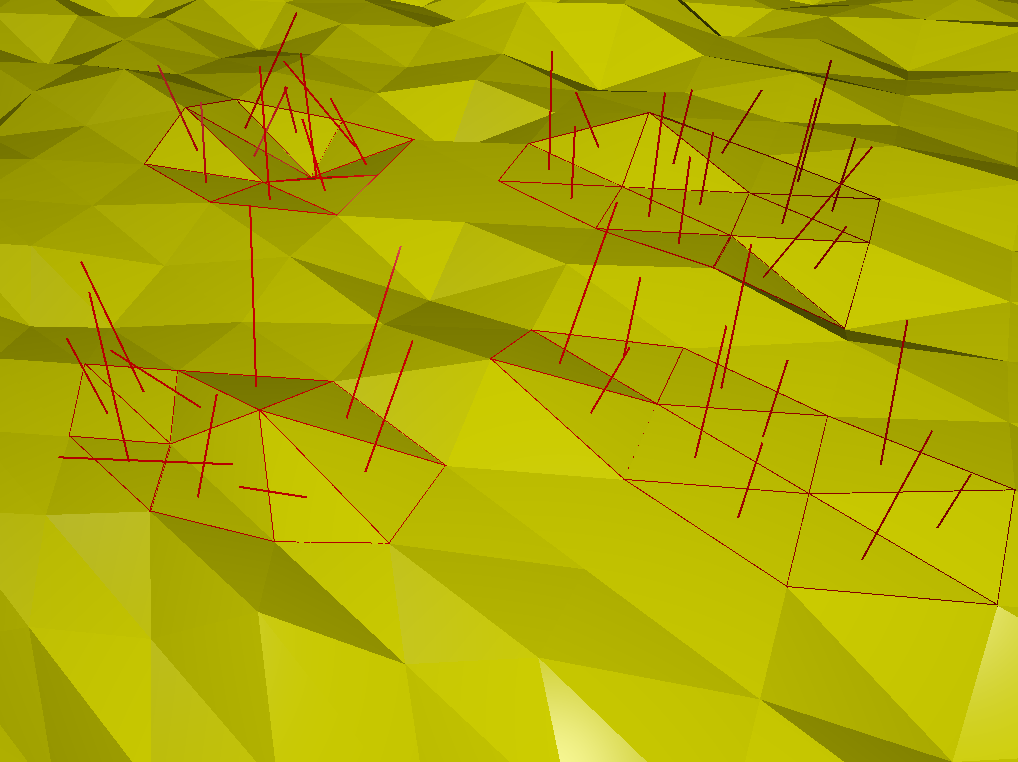
\includegraphics[scale=0.30]{figuras/validselection.png}
\caption{Uma seleção válida de \textit{patches} a serem utilizados no passo de pré-processamento. Em vermelho são mostradas as normais dos triângulos pertencentes aos \textit{patches} selecionados.}
\label{fig:validselection}
\end{figure}


Ainda no processo de deleção de \textit{patches}, a informação de fronteira de arestas é mantida para auxiliar na reconstrução dos elementos de $M'$. É então gerado um conjunto de arestas definido por:
\begin{equation} \label{eq:boundary} 
B = \{e : e \in (E_p \cap E')\}.
\end{equation}

\begin{figure}[!h]
\captionsetup{width=\linewidth}
\centering
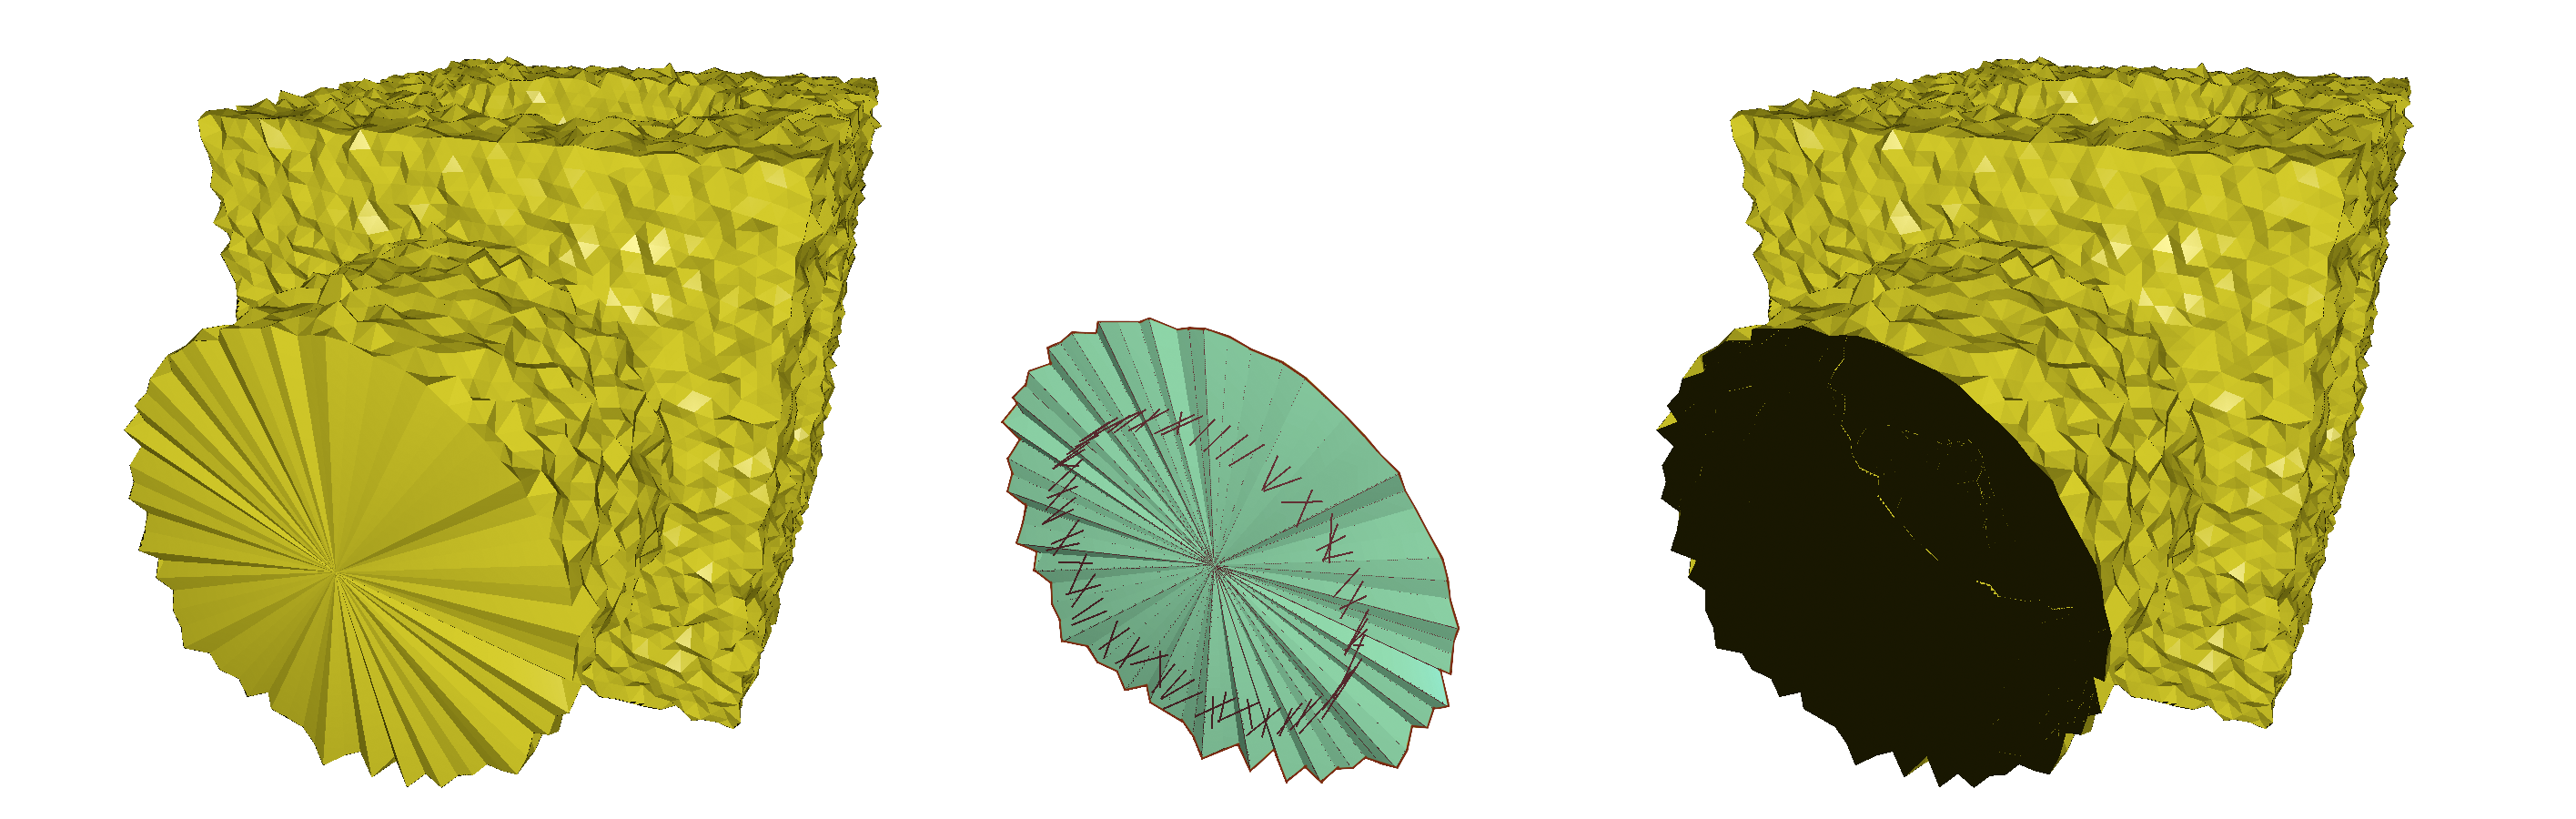
\includegraphics[width=\linewidth]{figuras/meshparts.png}
\caption{Exemplo do processo de seleção de \textit{patches} e criação de novas malhas. Da esquerda para a direita: malha original com ruído $M$, malha suporte $M_p$ e malha $M'$.}
\label{fig:meshparts}
\end{figure}

\subsubsection{Reconstrução}

O segundo passo do pré-processamento é a reconstrução de $M'$. É descrito em \cite{miranda2009surface} uma técnica de reconstrução de malhas de superfície que considera curvaturas e seu algoritmo foi utilizado nesse passo do pré-processamento. Esta técnica é essencialmente um algoritmo de avanço de fronteira que gera elementos, em superfícies arbitrárias, com a melhor forma possível. 


\begin{figure}[!h]
\captionsetup{width=\linewidth}
\centering
\includegraphics[width=\linewidth]{figuras/meshregenerationoverview.jpg}
\caption{Visão geral do processo de geração de malha de superfície descrito em \cite{miranda2009surface}.}
\label{fig:meshregeneration}
\end{figure}

A Figura \ref{fig:meshregeneration} mostra a visão geral do método de geração de malha proposto. A entrada para o algoritmo é uma descrição poligonal do contorno da superfície a ser gerada a malha e uma superfície de suporte que é representada abstratamente por três métodos:

\begin{itemize}  
\item \textit{Primeiro método:} Dada uma posição de um ponto, o método retorna o tamanho característico desejado de um triângulo equilátero ideal a ser criado com nesta posição. O tamanho do lado do triângulo é considerado como tamanho característico.
\item \textit{Segundo método:} Dada uma aresta corrente na fronteira atual, o método localiza o ponto \textit{apex} ideal que forma um novo triângulo. O método tem dois argumentos de entrada: a altura do triângulo equilátero candidato e um vetor unitário perpendicular à direção da aresta base. 
\item \textit{Terceiro método:} Dado um ponto no espaço, o método retorna o ponto da superfície suporte mais próximo ao ponto dado. Este método é usado apenas no estágio final da geração de malha para melhoria da malha local.
\end{itemize}

A técnica se inicializa com um processo de avanço de fronteira na região de borda definida pelo conjunto $B$ (Equação \ref{eq:boundary}) e continua até que toda a região esteja com uma malha gerada. Para cada aresta base na fronteira ativa, será criado um novo triângulo, processo esse realizado da seguinte forma:

\begin{itemize}
    \item A posição ideal para o vértice de um triângulo equilátero a ser formado é determinado usando o \textit{Primeiro} e \textit{Segundo} métodos. Usando o ponto médio da aresta base corrente como entrada, o tamanho do lado de um triângulo equilátero, a ser formado naquela posição, é retornado pelo \textit{Primeiro} método. Com este tamanho, a altura do triângulo candidato é obtida. Então fazendo o produto vetorial entre a normal à superfície e a aresta da fronteira, definido apenas por: \textbf{Normal} $\times$ \textbf{Tangente}, é descoberto o vetor unitário perpendicular a ser utilizado no \textit{Segundo} método, que então retorna a posição ideal para o novo ponto a ser gerado. A Figura \ref{fig:meshgeneration} ilustra este processo.
\end{itemize}

\begin{figure}[!h]
\captionsetup{width=\linewidth}
\centering
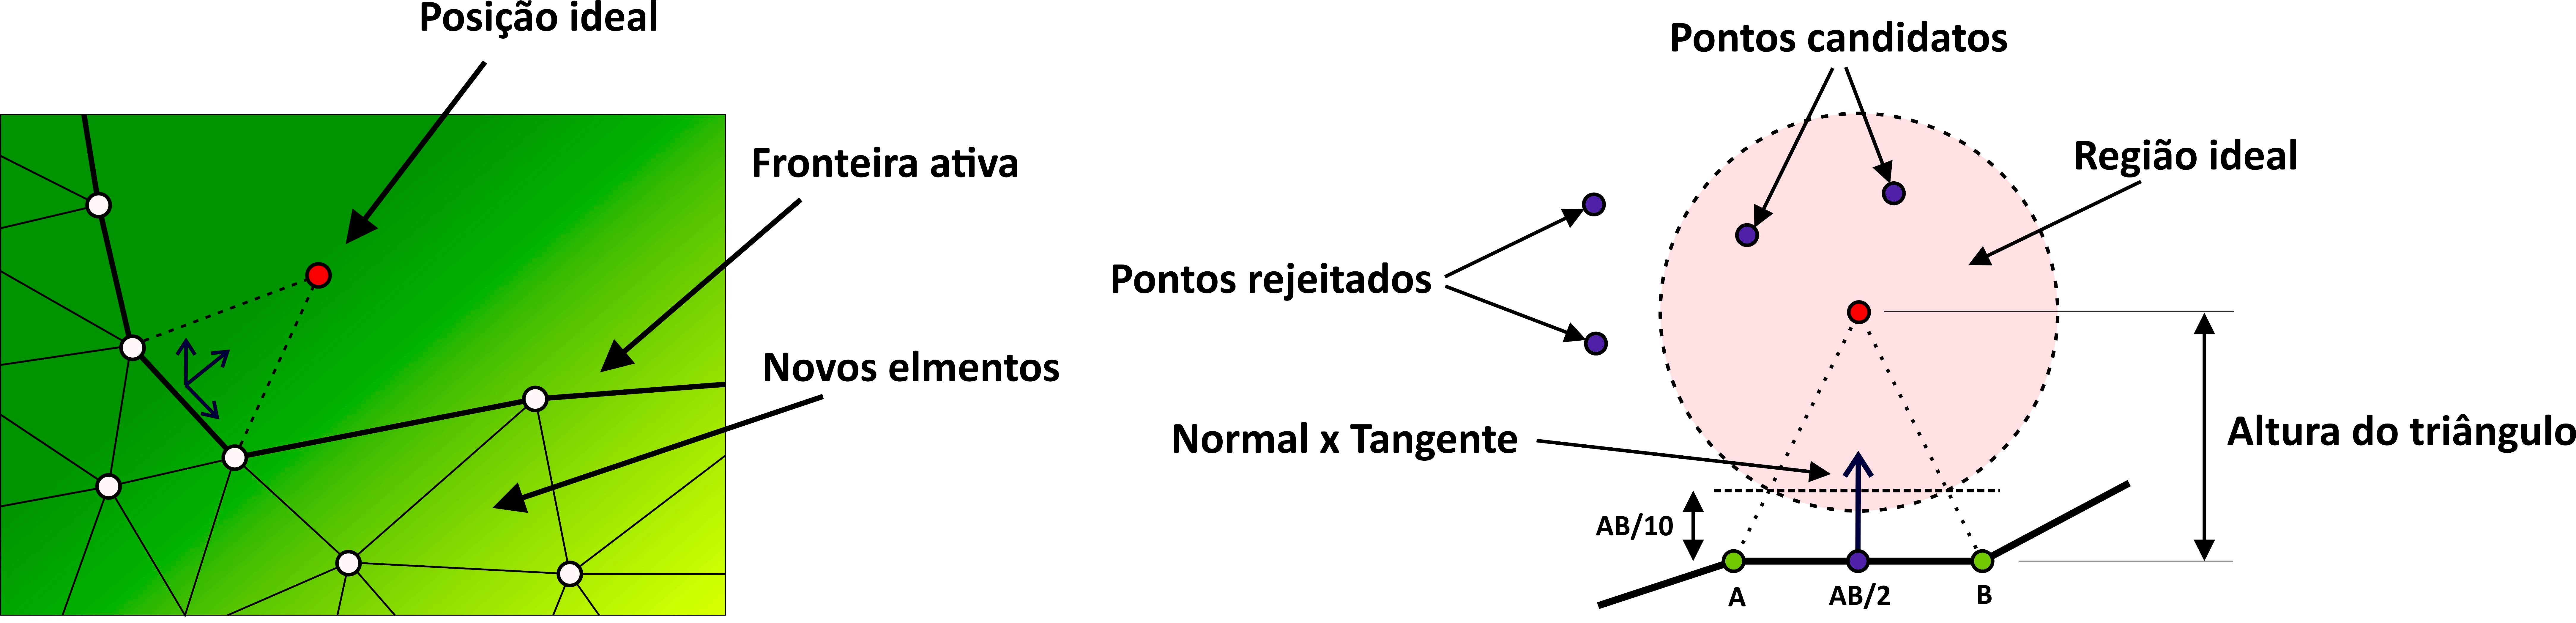
\includegraphics[width=\linewidth]{figuras/meshgeneration.jpg}
\caption{Processo de encontrar a posição de um ponto ideal para a criação de um novo triângulo.}
\label{fig:meshgeneration}
\end{figure}


Como último passo, um processo de suavização é aplicado para aprimorar a qualidade da malha. Uma formulação para este passo é dado na Equação \ref{eq:meshlaplacian}, que é uma forma geral de um \textit{Laplaciano} com pesos atribuídos:

\begin{equation} \label{eq:meshlaplacian}
    X^{n+1}_O = X^{n}_O + \phi \frac{\sum^{m}_{i=1} w_{iO}(X^{n}_i - X^{n}_O) }{\sum^{m}_{i=1} w_{iO}},
\end{equation}
onde $m$ representa a quantidade de vértices conectados ao vértice $O$, $X^{n+1}_O$ é a posição do vértice $O$ na iteração $n+1$, $w_{iO}$ é o peso atribuído entre os vértices $i$ e $O$, e $\phi$ é um parâmetro de relaxamento normalmente determinado entre $(0,1]$. Em \cite{miranda2009surface} foi observado bons resultados com $\phi = w_{iO} = 1.0$, fazendo com que apenas os vértices adjacentes influenciem o vértice $O$. Esse processo de suavização geralmente faz com que os vértices se distanciem da superfície suporte. O \textit{Terceiro} método é utilizado com o intuito de reposicionar os vértices de volta à superfície suporte. Maiores detalhes podem ser encontrados em \cite{miranda2009surface}. 

Ao final deste processo de reconstrução, teremos como resultado uma malha $M_0$ com ruído, completamente pré-processada e pronta para ser utilizada no passo seguinte de remoção de ruídos do modelo.


\subsection{Processo de filtragem para otimização da malha}

Após o pré-processamento da malha, será utilizada uma técnica de remoção de ruídos no modelo que consistirá essencialmente em dois passos:

\begin{itemize}
    \item Aplicação da filtragem bilateral das normais das faces da malha;
    \item Reposicionamento dos vértices de acordo com as normais filtradas no passo anterior.
\end{itemize}


\subsubsection{Filtragem bilateral das normais das faces}

Manter as características do modelo é um grande desafio em uma técnica de filtragem bilateral. Filtrar diretamente os vértices da malha como descrito em \cite{fleishman2003bilateral} e \cite{jones2003non} pode ocasionar perdas de características importantes dependendo do modelo. Normais das faces de uma malha fornecem descrições mais precisas das características geométricas de um modelo. Uma aresta de borda pode ser detectada simplesmente calculando a diferença entre as normais das faces incidentes, como é ilustrado na Figura \ref{fig:meshsharpedge}. 

\begin{figure}[!h]
\captionsetup{width=\linewidth}
\centering
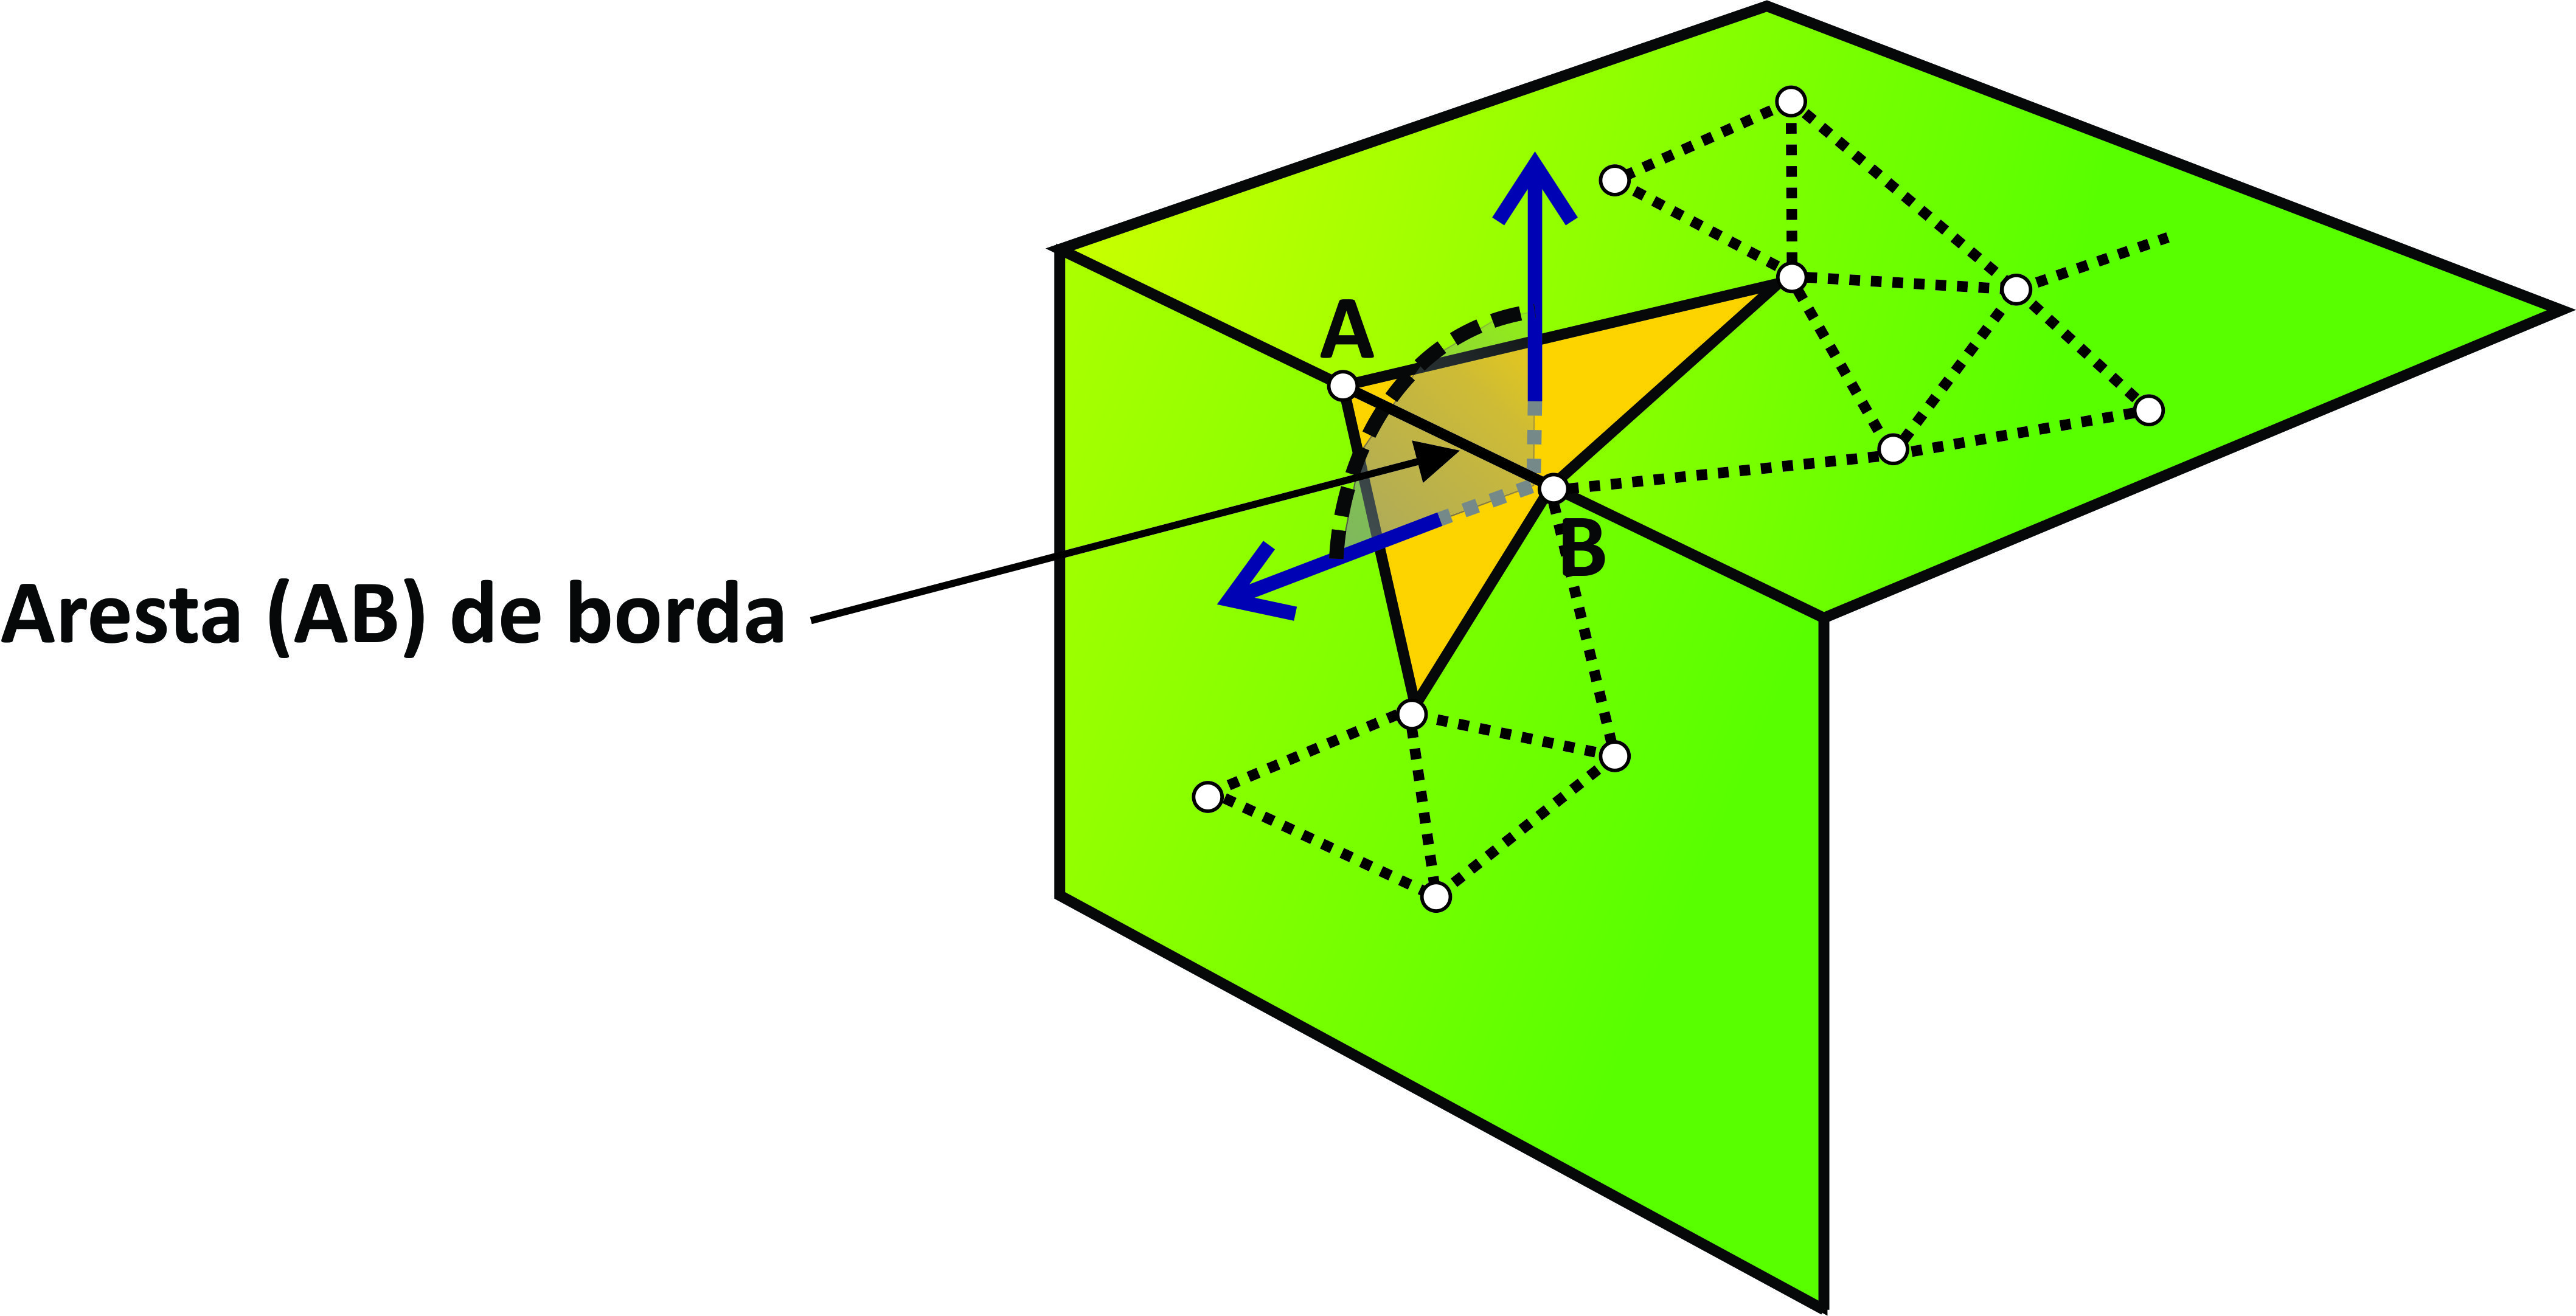
\includegraphics[width=\linewidth]{figuras/meshsharpedge.jpg}
\caption{Aresta AB de borda detectada pela grande diferença entre as normais das suas duas faces incidentes.}
\label{fig:meshsharpedge}
\end{figure}


Quando uma malha não possui ruído, as normais das faces podem fornecer um bom sinal guia na filtragem bilateral, no entanto, em um modelo com ruído, essa informação é perdida devido a grande divergência das normais presentes. O exemplo na Figura \ref{fig:meshpatchnormals} mostra que duas normais de triângulos vizinhos, compartilhando uma aresta, ainda podem ter valores muito divergentes de direção e essa aresta não ser de borda. É necessário então criar um conjunto de normais guia mais robusto que forneça informações geométricas mais precisas na presença de ruído.

\begin{figure}[!h]
\captionsetup{width=\linewidth}
\centering
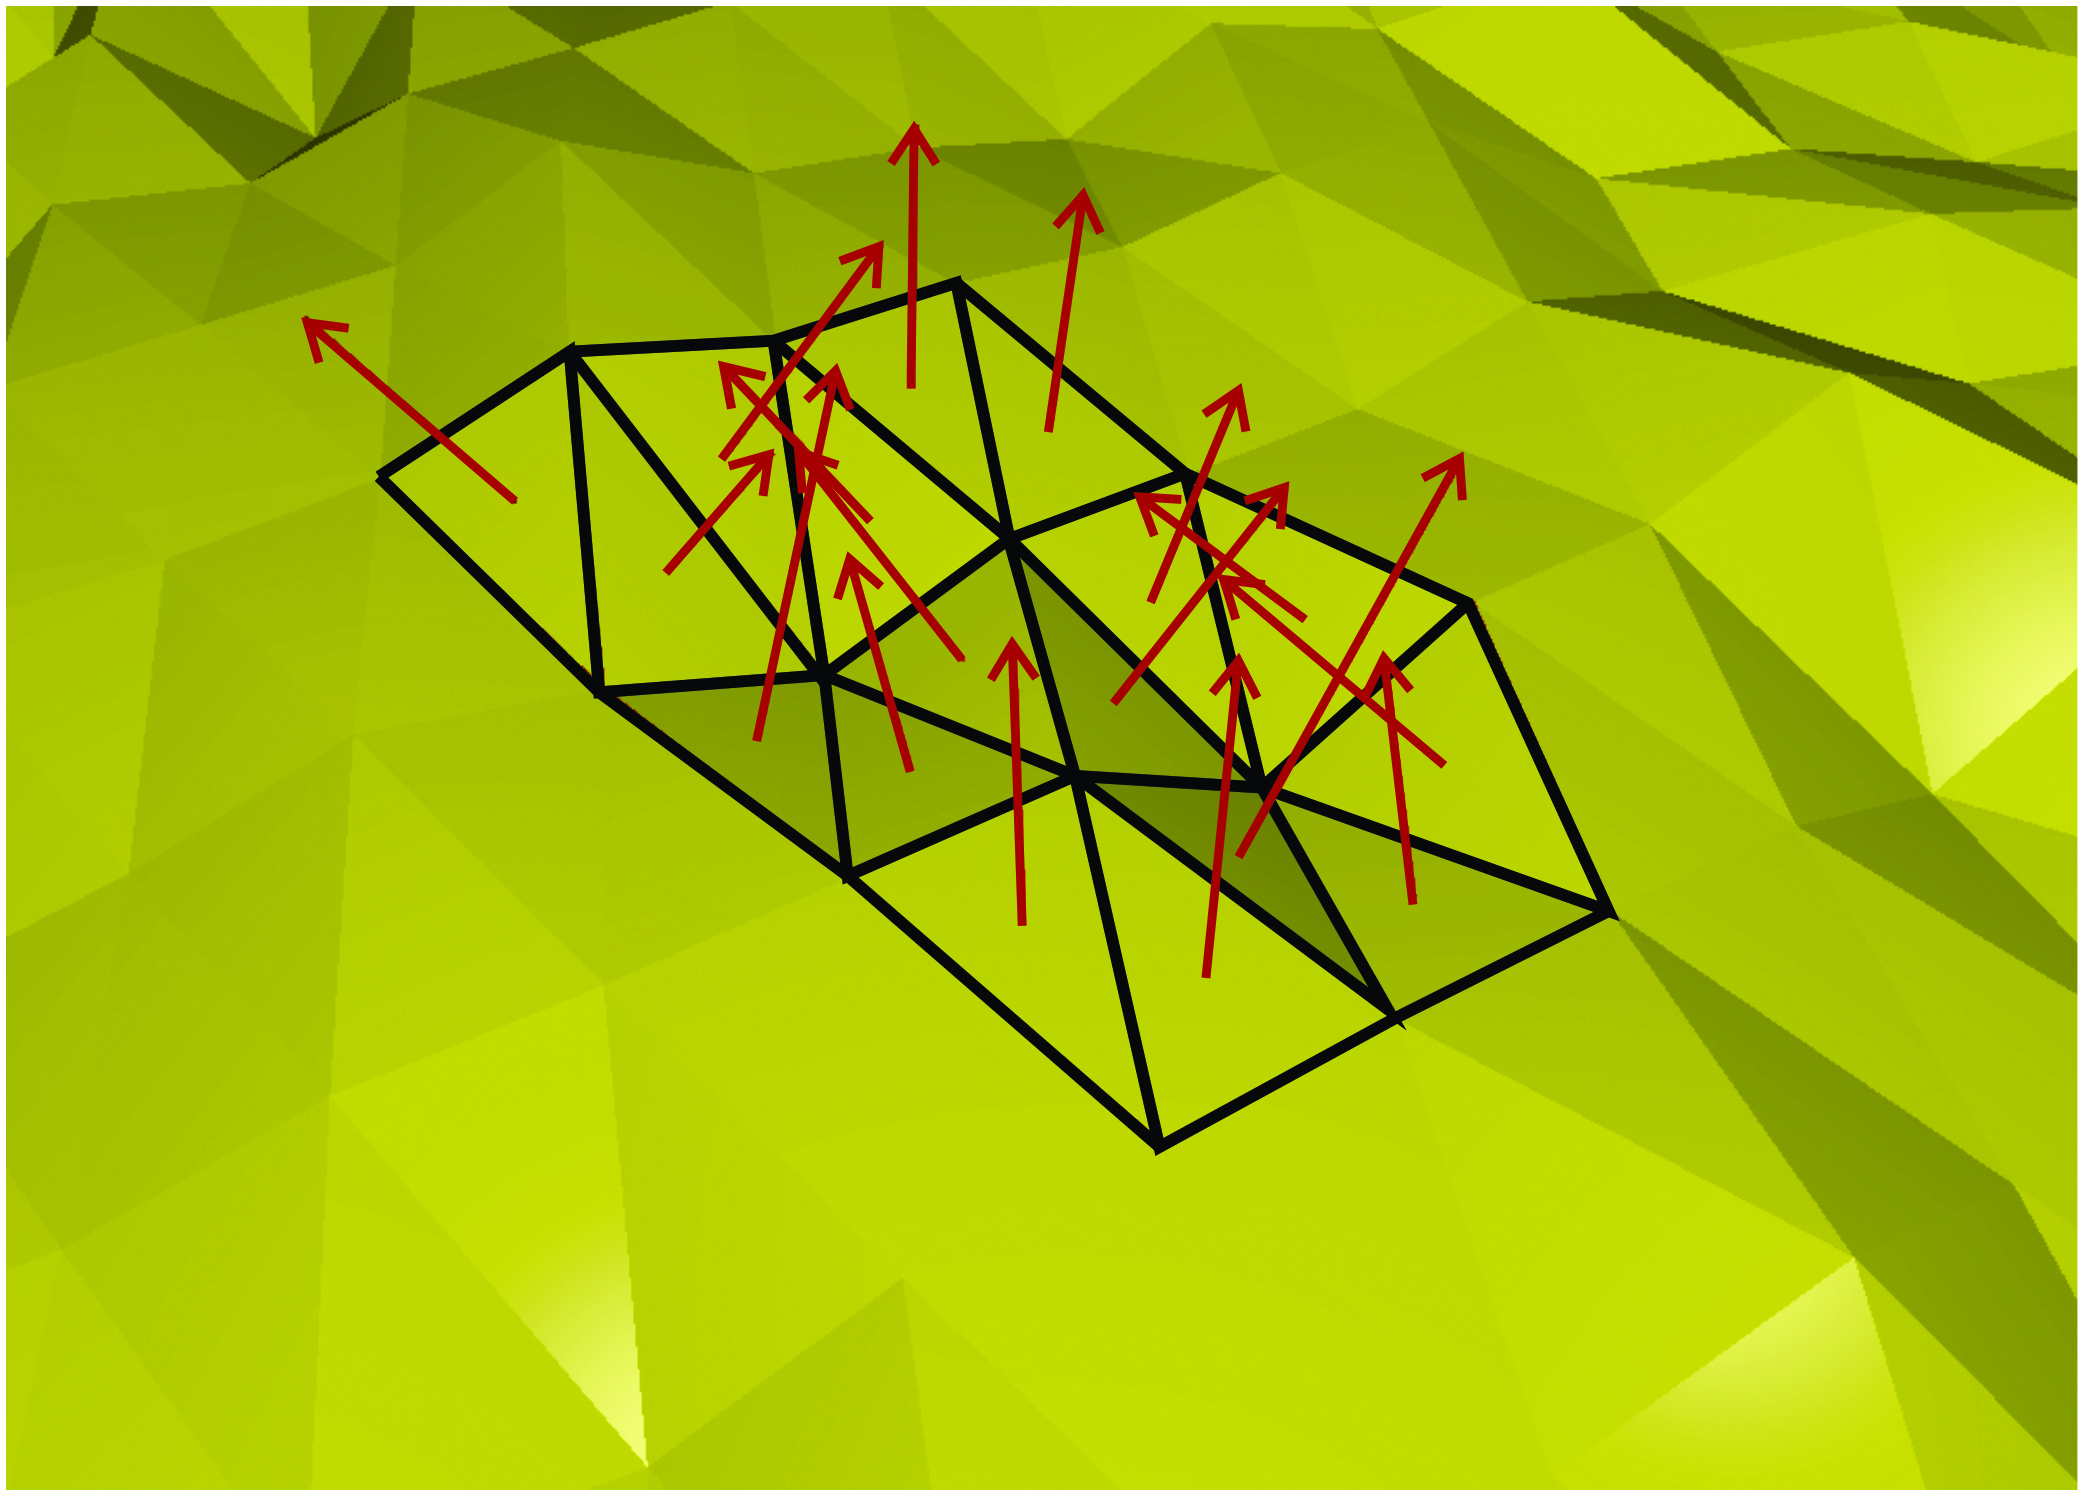
\includegraphics[scale=0.83]{figuras/meshnormals.jpg}
\caption{Um \textit{patch} de triângulos de um modelo com ruído mostrando a divergência das normais de suas faces. Dessa forma, as normais não funcionam como um sinal guia confiável para a filtragem bilateral e não indicam informações geométricas precisas.}
\label{fig:meshpatchnormals}
\end{figure}

Um modelo baseado em malha pode ser decomposto em vários pequenos \textit{patches}, cada um consistindo de múltiplas faces com normais de direção similar. Decompor uma malha dessa forma não é intuitivo. Foi usado o mesmo processo descrito em \cite{zhang2015guided}: para cada face $f_k$ é definido um \textit{patch} $P_k$ como a união de $f_k$ e suas faces vizinhas que compartilham pelo menos um vértice com $f_k$. Para achar a normal guia de uma face $f_i$ é procurado dentre todos os \textit{patches} que $f_i$ faz parte, aquele que possui normais mais semelhantes, e então a normal média desse \textit{patch} é atribuída a $f_i$. O conjunto de \textit{patches} candidatos pode ser definido como:
\begin{equation}
    C(f_i) = \{P_k | f_i \in P_k\}.
\end{equation}
Para cada \textit{patch} $P \in C(f_i)$, é definida uma função de consistência que calcula o quão similares as normais no \textit{patch} $P$ são:
\begin{equation} \label{eq:consistencyfunc}
    H(P) = \Phi(P)\cdot R(P),
\end{equation}
onde $\Phi(P)$ mede a diferença máxima entre duas normais do \textit{patch}:
\begin{equation}
    \Phi(P) = \mathop{max}_{f_j,f_k \in P} \|\textbf{n}_j - \textbf{n}_k \| 
\end{equation}
e $R(P)$ é uma medida relativa de saliência de aresta no \textit{patch}:
\begin{equation}
    R(P) = \frac{max_{e_j\in E_p} \upvarphi(e_j)}{ \upvarepsilon + \sum_{e_j\in E_p}{\upvarphi(e_j)} },
\end{equation}
onde $E_p$ é o conjunto de arestas com ambas as faces incidentes contidas no \textit{patch} P (Figura \ref{fig:epedges}), $\upvarphi(e_j)$ mede a saliência de uma aresta $e_j$ pela diferença entre as normais das duas faces incidentes $f_{j_1}$ e $f_{j_2}$:
\begin{equation}
    \upvarphi(e_j) = \|\textbf{n}_{j_1} - \textbf{n}_{j_2} \|,
\end{equation}
e $\upvarepsilon$ é um valor positivo e pequeno para evitar divisões por $0$.

\begin{figure}[!h]
\captionsetup{width=\linewidth}
\centering
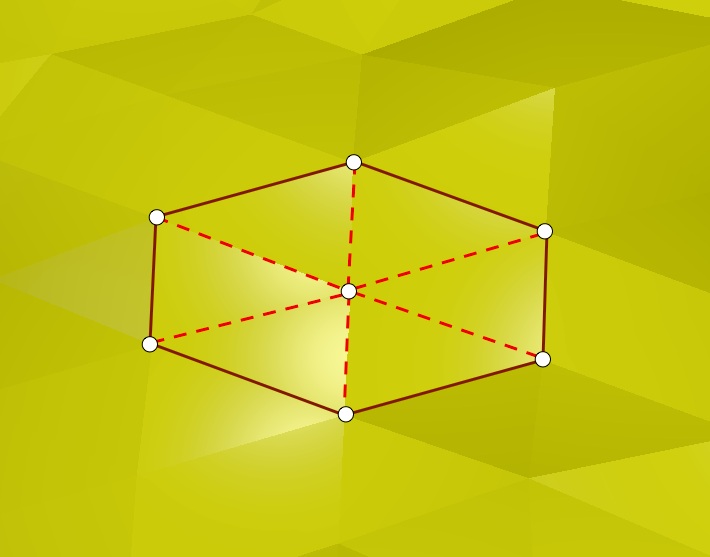
\includegraphics[scale=0.30]{figuras/E_pEdges.png}
\caption{Um \textit{patch} de faces e suas arestas. Linhas tracejadas ilustram as arestas pertencentes ao conjunto $E_p$.}
\label{fig:epedges}
\end{figure}

Entre todos os \textit{patches} candidatos para $f_i$, é escolhido o \textit{patch} $P^*$ que possui o menor valor para a função de consistência e é então computada a sua normal média $\mathbf{g}_i$, ponderada pela área das faces contidas no \textit{patch}:
\begin{equation}
    \mathbf{g}_i = \frac{ \sum_{f_j \in P^*}{A_j\mathbf{n}_j} }{ \|\sum_{f_j \in P^*}{A_j\mathbf{n}_j}\| },
\end{equation}
onde $A_j$ é a área da face $f_j$. Todo o processo é ilustrado na Figura \ref{fig:guidedzangconsistencyfunction}.

\begin{figure}[!h]
\captionsetup{width=\linewidth}
\centering
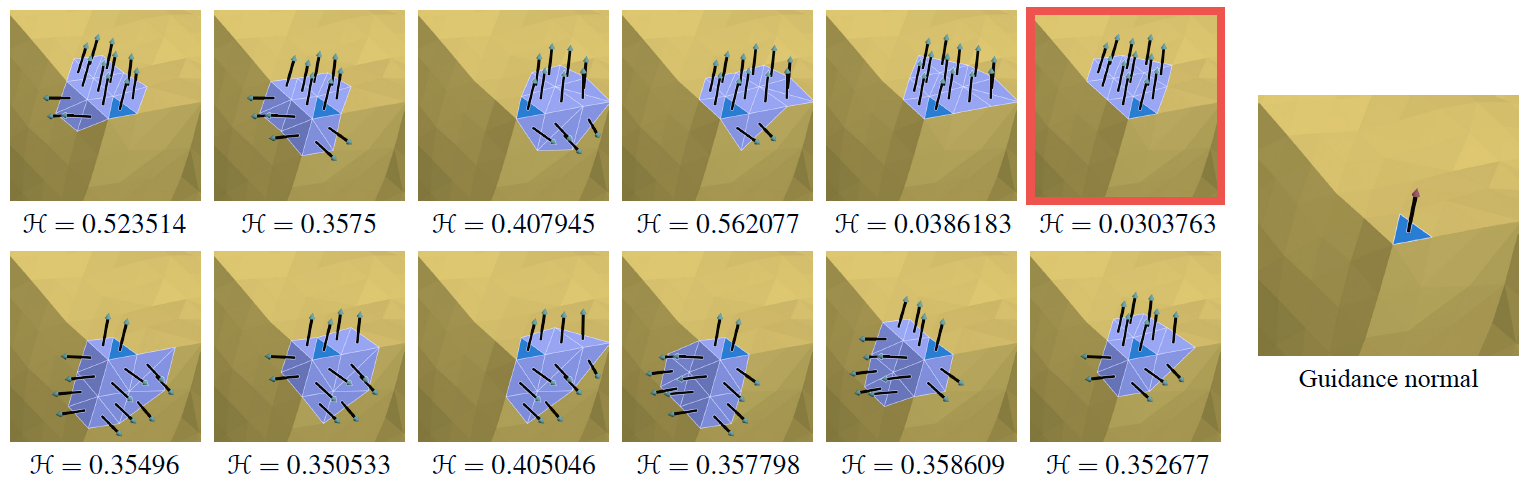
\includegraphics[width=\linewidth]{figuras/guidedzangconsistencyfunction.png}
\caption{Cálculo da função de consistência para todos os \textit{patches} que a face $f_i$ (em azul) está contida. O \textit{patch} $P$ com menor valor (destacado em vermelho) de função de consistência $H(P)$, calculado pela Equação \ref{eq:consistencyfunc}, será o escolhido, e sua normal média será atribuída à face $f_i$.}
\Fonte{\cite{zhang2015guided}}
\label{fig:guidedzangconsistencyfunction}
\end{figure}


Após a construção do conjunto de normais guia para toda a malha, o processo de filtragem irá prosseguir. Para cada face $f_i$, com vetor normal unitário $n_i$, centróide $c_i$, e normal guia $g_i$, é computado a normal filtrada $\overline{n}_i$ pelo seguinte filtro bilateral:
\begin{equation} \label{eq:filtrobilateraldasnormais}
    \overline{n}_i = \frac{1}{W_i}\sum_{f_j \in \mathcal{N}_i}{A_j K_s(c_i,c_j)K_r(g_i,g_j) n_j},
\end{equation}
onde $\mathcal{N}_i$ é o conjunto de faces na vizinhança de $f_i$; $A_j$ é a área da face $f_j$; \textbf{$K_s$} e \textbf{$K_r$} são os \textit{kernels} espacial e de distância respectivamente; \textbf{$n_j$} é a normal da face $f_j$ e $W_i = \|\sum_{f_j \in \mathcal{N}_i}{A_j K_s(c_i,c_j)K_r(g_i,g_j) n_j}\|$ é um fator de normalização para garantir que a normal filtrada será um vetor unitário. Para este trabalho, foram usadas as seguintes funções para \textbf{$K_s$} e \textbf{$K_r$}:
\begin{equation}
    K_s(c_i,c_j) = exp(-\frac{ {\| c_i-c_j \|}^2 }{ 2{\sigma_s}^2 }),
\end{equation}
\begin{equation}
    K_r(g_i,g_j) = exp(-\frac{ {\| g_i-g_j \|}^2 }{ 2{\sigma_r}^2 }),
\end{equation}
onde os parâmetros de variância \textbf{$\sigma_s$} e \textbf{$\sigma_r$} controlam a zona de influência dos \textit{kernels}. O conjunto $\mathcal{N}_i$ contém a face $f_i$ e suas faces vizinhas (Figura \ref{fig:facesvizinhas}). Elas podem ser definidas como:
\begin{itemize}
    \item \textbf{Vizinhas imediatas:} faces que compartilham pelo menos um vértice com $f_i$.
    \item \textbf{Vizinhas próximas:} faces cujo centróide está a uma distância $r$ do centróide de $f_i$.
\end{itemize}


\begin{figure}[!h]
\captionsetup{width=\linewidth}
\centering
\includegraphics[width=\linewidth]{figuras/facesvizinhas.png}
\caption{Diferença da definição de vizinhança. A esquerda temos a vizinhança imediata de $f_i$; a direita, a vizinhança próxima de $f_i$, onde o parâmetro $r$, que representa o raio, é definido pelo usuário.}
\label{fig:facesvizinhas}
\end{figure}


\subsubsection{Atualizando vértices}

Após o processo de filtragem das normais, os vértices da malha têm que ser atualizados para corresponder às novas normais calculadas na Equação \ref{eq:filtrobilateraldasnormais}. Aqui foi usado o mesmo procedimento descrito em \cite{zhang2015guided} e \cite{sun2007fast}: para cada face $f_i$ com posições de vértice: $\overline{v}_{ix}$, $\overline{v}_{iy}$ e $\overline{v}_{iz}$, elas serão atualizadas pela seguinte iteração:
\begin{equation}
	\overline{v}^{(k+1)}_{i} = \overline{v}^{(k)}_{i} + \frac{1}{|\mathcal{F}_i|} \sum_{j \in \mathcal{F}_i}{ \overline{n}_j \Big[ \overline{n}_j \cdot \Big( \overline{c}^{(k)}_j - \overline{v}^{(k)}_i \Big) \Big] },
\end{equation}
onde $\overline{v}^{(k)}_{i}$ representa o valor de $\overline{v}_{i}$ na $k$-ésima iteração, $\mathcal{F}_i$ é o conjunto de índices das faces incidentes para o vértice $\overline{v}_{i}$ e $\overline{c}^{(t)}_j$ é o centróide de $f_i$ na $k$-ésima iteração. Esse procedimento é intercalado $k$ vezes com a filtragem das normais até que um resultado satisfatório seja obtido. Nos exemplos mostrados no capítulo seguinte, $k \in [10, 20]$ obteve bons resultados.

O Algoritmo ~\ref{alg:finalmainalg} sumariza toda a técnica proposta no presente trabalho, mostrando os passos principais e omitindo detalhes que já foram discutidos ao longo do capítulo.

\begin{algorithm}[]
\SetKwInOut{Input}{Input}\SetKwInOut{Output}{Output}
\Input{Malha inicial $\mathbf{M}$, número de iterações $k$}
\Output{Malha $\mathbf{M_{k}}$ sem ruídos}
\BlankLine

    Selecione \textit{patches} \{p\} de faces em $\mathbf{M}$\;
    Delete o conjunto \{p\} de $\mathbf{M}$ gerando $\mathbf{M'}$ e $\mathbf{M_p}$\;
    Construa o conjunto $\mathbf{B}$ de fronteiras\;
    Gere $\mathbf{M_0}$ reconstruindo $\mathbf{M'}$ a partir de $\mathbf{B}$ e $\mathbf{M_p}$\;
    
    \Para{i = 1 até k}{
        Construa o conjunto de normais guia \{$\mathbf{g_i}$\}\;
        Compute as normais filtradas \{$\mathbf{\overline{n}_i}$\}\;
        Atualize os vértices de $\mathbf{M_i}$ de acordo com \{$\mathbf{\overline{n}_i}$\}\;
	}
    retorne $\mathbf{M_{k }}$\;
\caption{Filtragem Bilateral das normais da malha com passo de pré-processamento}
\label{alg:finalmainalg}
\end{algorithm}

	\chapter{Exemplos e resultados}
\label{chap:exemploseresultados}

Neste capítulo são apresentados os resultados de aplicação da técnica proposta nesse trabalho em alguns modelos. É mostrada a diferença da sua utilização na remoção de ruídos de um modelo. Os resultados para a técnica descrita neste trabalho são nomeados como \textit{pre-guided} e comparados com os resultados obtidos pelos trabalhos de \cite{zhang2015guided}, \cite{sun2007fast} e \cite{zheng2011bilateral}, que serão denotados como \textit{guided}, \textit{fast-and-effective} e \textit{bilateral-normal-filtering}.

A técnica descrita neste trabalho foi implementada em C++, utilizando a biblioteca de API gráfica livre \textit{modern OpenGL} (Open Graphics Library), libigl (https://github.com/libigl/libigl), GLEW, glfw e assimp.

O computador utilizado para a técnica foi um MacBook Air, com processador Intel Core i5, 1.3 GHz, 8 GB de memória DDR3 1600 MHz e placa de vídeo Intel HD Graphics 5000 com 1546 MB de memória gráfica.

\section{Modelos}

Ao todo, foram utilizados 4 modelos, sendo 3 modelos com ruído artificial e regiões com triangulação de baixa qualidade e 1 modelo digitalizado do mundo real para mostrar a eficiência da técnica em problemas reais. Eles serão referidos como: \textit{block}, \textit{carter}, \textit{mechanic} e \textit{angel} (Figura \ref{fig:models}). 

\begin{figure}[!h]
\captionsetup{width=\linewidth}
\centering
\includegraphics[width=\linewidth]{figuras/models.png}
\caption{Modelos utilizados na técnica proposta. Na primeira metade da imagem temos \textit{block} e \textit{carter}, seguidos do modelo \textit{mechanic} em duas visões diferentes. Mais a direita temos o modelo \textit{angel} que foi digitalizado do mundo real a partir de um \textit{scanner} 3D.}
\label{fig:models}
\end{figure}

\begin{figure}[!h]
\captionsetup{width=\linewidth}
\centering 
\includegraphics[scale=0.34]{figuras/artificialnoise.png}
\caption{Processo de criação dos modelos de entrada. A esquerda temos os modelos \textit{ground-truth}: \textit{block}, \textit{carter} e \textit{mechanic} em duas visões diferentes. As regiões em destaque representam a zona onde a qualidade de triangulação foi propositalmente reduzida. A direita tem-se o segundo passo da criação dos modelos artificiais: a aplicação de um ruído branco aleatório e artificial ao longo das normais dos vértices.}
\label{fig:artificialnoise}
\end{figure}

Para mostrar a robustez da técnica apresentada, utilizamos dois processos na criação dos 3 primeiros modelos de entrada:
\begin{itemize}
    \item Algumas regiões do modelo foram reconstruídas, deixando a triangulação com qualidade ruim.
    \item Um processo de ruído artificial é aplicado. Os vértices são movidos a uma pequena distância aleatória (positiva ou negativa) na direção da sua normal.
\end{itemize}

Ao final deste processo, ilustrado na Figura \ref{fig:artificialnoise}, terão-se os 3 modelos com as duas pré-condições suficientes para que a técnica proposta mostre bons resultados em relação às demais. 

\section{Métricas de Qualidade}\label{metrics}

Para medir qualidade e eficiência em uma técnica de remoção de ruídos, a grande maioria dos artigos na literatura seguem o seguinte padrão:
\begin{itemize}
    \item Uma malha sem ruído, chamada \textit{ground-truth}, é adquirida.
    \item É aplicado um ruído sintético na \textit{ground-truth}.
    \item A técnica é aplicada obtendo uma malha resultante.
    \item Métricas de comparação são executadas entre a malha resultante e a \textit{ground-truth}.
\end{itemize}

Dessa forma, é medido o quão semelhante a malha resultante ficou da sua forma esperada. Uma forma de medir essa semelhança é calcular a proximidade da malha resultante com a \textit{ground-truth}.

A métrica de qualidade mais comum na literatura é a \textit{distância de erro média} (MDE), definida para uma malha resultante $X$ e uma malha \textit{ground-truth} $G$, pela seguinte equação:
\begin{equation}
    MDE(X,G) = \frac{1}{n} \sum_{i=1}^{n}{\|x_i - g_i \|}, 
\end{equation}
onde $n$ é o número de vértices em ambas as malhas, $x_i$ é um vértice da malha resultante e $g_i$ é o mesmo vértice na malha \textit{ground-truth}. Essa métrica simplesmente calcula a distância média que cada vértice está do resultado ideal (\textit{ground-truth}). Quanto mais próximo o $MDE(X,G)$ estiver de $0$, mais eficiente será a técnica. Como a técnica proposta tem um passo de pré-processamento, em geral a malha resultante vai possuir mais vértices do que a malha \textit{ground-truth}, então essa métrica não deve ser usada diretamente, pois estariam-se ignorando informações relevantes na medida de erro.

Para este fim, como medida de qualidade, foi usado a técnica presente em \cite{cignoni1998metro} para estimar o erro em nosso processo de remoção de ruídos. Esta técnica faz amostragens de pontos na superfície da malha resultante e calcula a distância mínima entre esses pontos e a malha \textit{ground-truth} basedo na distância de \textit{Hausdorff}.

A distância de \textit{Hausdorff}, ilustrada na Figura \ref{fig:hausdorffdistance}, mede o quão distante dois conjuntos de um espaço métrico estão um do outro. Seja $X$ e $Y$ dois subconjuntos não vazios de um espaço métrico. A distância de \textit{Hausdorff} $d_H(X,Y)$ é definida por:
\begin{equation}
	d_H(X,Y) = \max \{ {\sup_{x \in X}} \: {\inf_{y \in Y}} \: d(x,y), \underset{y \in Y}{\sup} \: \underset{x \in X}{\inf} \: d(x,y) \},
\end{equation}
onde $sup$ representa o \textit{supremum}, $inf$ o \textit{infimum} e $d(x,y)$ representa a distância entre os pontos $x \in X$ e $y \in Y$.

\begin{figure}[!h]
\captionsetup{width=\linewidth}
\centering
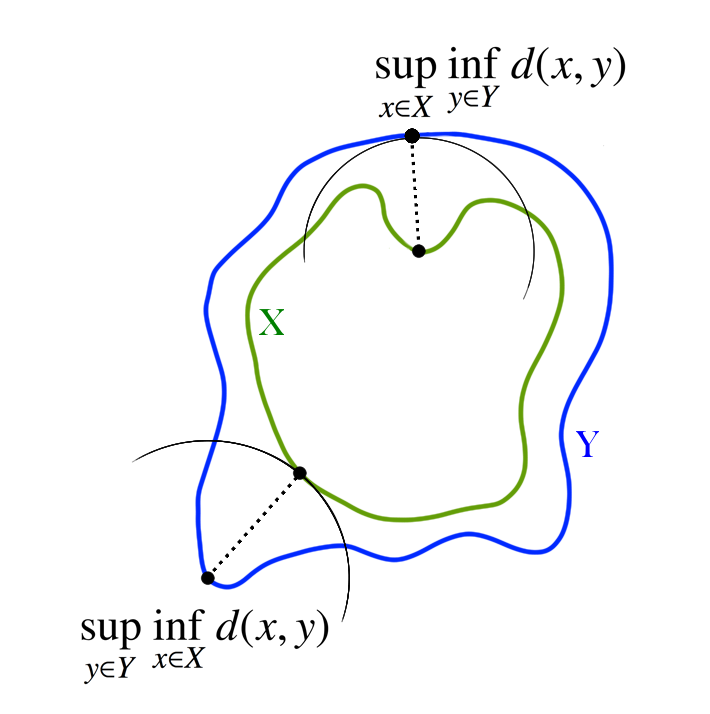
\includegraphics[scale=0.4]{figuras/Hausdorff_final.png}
\caption{A distância de \textit{Hausdorff} entre dois subconjuntos $X$ e $Y$: $d_H(X,Y)$ irá resultar na maior das duas distâncias.}
\label{fig:hausdorffdistance}
\end{figure}

A distância de \textit{Hausdorff} $d_H(X,Y)$ é um valor que representa a distância entre dois subconjuntos. Já que estamos interessados na distância mínima entre cada ponto amostrado na malha resultante, a distância de \textit{Hausdorff} modificada (MHD) para um ponto amostrado $x$ na malha resultante $X$ e a malha \textit{ground-truth} $G$, será definido por:
\begin{equation}
	MHD(x,G) = \underset{g \in G}{\inf} \: d(x,g),
\end{equation}
onde $g$ é o ponto na superfície da malha $G$ que produz a menor distância para $x$. Portanto $MHD(x,G)$ será o resultado da menor distância de um ponto $x$ para a malha $G$. 

Estendendo este conceito para todos os pontos amostrados: seja $n_s$ o número de pontos amostrados na superfície da malha $X$, $x_i$ um ponto amostrado na superfície de $X$ e $g$ o ponto na superfície da malha $G$ que produz a menor distância para $x_i$. Será definida então a distância de \textit{Hausdorff} modificada média (MMHD):
\begin{equation} \label{eq:mmhd}
	MMHD(X,G) = \frac{1}{n_s} \sum_{i=1}^{n_s}{MHD(x_i,G)},
\end{equation}
que conterá a média entre todos os MHD dos pontos amostrados, representando assim a média da distância que a malha resultante está da malha ideal (\textit{ground-truth}).

Apesar da $MMHD$ ser uma métrica mais precisa, irá se usar também a razão entre os volumes da malha resultante e da \textit{ground-truth} para informações mais concisas e completas sobre a validez da técnica proposta. Ao todo serão usadas quatro métricas:

\begin{itemize} 
    \item \textbf{MHD mínimo}: O menor valor de MHD entre todos os pontos amostrados. Esse valor representa o deslocamento mínimo de um ponto na malha resultante causado pela técnica. Valores próximos ou iguais a 0 são preferíveis.
    \item \textbf{MHD máximo}: O maior valor de MHD entre todos os pontos amostrados. Esse valor representa o deslocamento máximo de um ponto na malha resultante causado pela técnica. Valores próximos ou iguais a 0 são preferíveis.
    \item \textbf{MMHD}: O valor médio de todos os valores de MHD dos pontos amostrados como definido em \ref{eq:mmhd}. Valores próximos ou iguais a 0 são preferíveis. Esta é a métrica mais importante.
    \item \textbf{Proporção de Volume}: A razão de proporção entre o volume do modelo resultante e o volume do modelo \textit{ground-truth}. Quanto mais próximo esse valor for de 1, melhor.
\end{itemize}


\section{Resultados}
\label{sec:resultados}

Na sequência, será comparado a técnica proposta com \cite{zhang2015guided}, \cite{sun2007fast} e \cite{zheng2011bilateral}, aplicando as quatro técnicas nos modelos de ruído sintético mostrados na Figura \ref{fig:models}, e utilizando as quatro medidas de qualidade descritas na seção \ref{metrics} para comparação. Todos os modelos foram amostrados com 6000000 de pontos na sua superfície para o cálculo do MMHD. As Figuras \ref{fig:block_final}, \ref{fig:carter_final}, \ref{fig:mechanic1_final} e \ref{fig:mechanic2_final} mostram os resultados finais das técnicas citadas aplicadas aos quatro modelos propostos, mostrando assim a comparação da técnica proposta nesse trabalho com as demais. As Figuras \ref{fig:block_hausdorff_final}, \ref{fig:carter_hausdorff_final}, \ref{fig:mechanic1_hausdorff_final} e \ref{fig:mechanic2_hausdorff_final} ilustram a visualização das distâncias de \textit{Hausdorff} dos 6 milhões de pontos amostrados, assim como um histograma de distribuição desses pontos. O modelo \textit{angel}, que possui ruído real, não possui uma malha \textit{ground-truth} de comparação, portanto usou-se a técnica proposta para mostrar que visualmente ele possui uma melhor qualidade, como é notado nas Figuras \ref{fig:angel_final} e \ref{fig:angel_detail}.



\begin{figure}[p]
\captionsetup{width=\linewidth}
\centering
\includegraphics[width=16cm]{figuras/block_final.png}
\caption{Comparação da técnica proposta com as técnicas de \cite{zhang2015guided}, \cite{sun2007fast} e \cite{zheng2011bilateral} para o modelo \textit{block}. Primeira linha: \textit{ground-truth}, \textit{ground-truth} com malha, modelo com ruído sintético, modelo com ruído sintético e malha. Segunda linha: técnicas de \cite{zhang2015guided}, \cite{sun2007fast}, \cite{zheng2011bilateral} e a técnica proposta, respectivamente. Terceira linha: as mesmas técnicas da linha anterior mostrando as malhas dos modelos.}
\label{fig:block_final}
\end{figure}

\clearpage

\begin{figure}[p]
\captionsetup{width=\linewidth}
\centering
\includegraphics[width=16cm]{figuras/carter_final.png}
\caption{Comparação da técnica proposta com as técnicas de \cite{zhang2015guided}, \cite{sun2007fast} e \cite{zheng2011bilateral} para o modelo \textit{carter}. Primeira linha: \textit{ground-truth}, \textit{ground-truth} com malha, modelo com ruído sintético, modelo com ruído sintético e malha. Segunda linha: técnicas de \cite{zhang2015guided}, \cite{sun2007fast}, \cite{zheng2011bilateral} e a técnica proposta, respectivamente. Terceira linha: as mesmas técnicas da linha anterior mostrando as malhas dos modelos.}
\label{fig:carter_final}
\end{figure}

\clearpage

\begin{figure}[p]
\captionsetup{width=\linewidth}
\centering
\includegraphics[width=16cm]{figuras/mechanic1_final.png}
\caption{Comparação da técnica proposta com as técnicas de \cite{zhang2015guided}, \cite{sun2007fast} e \cite{zheng2011bilateral} para o modelo \textit{mechanic}. Primeira linha: \textit{ground-truth}, \textit{ground-truth} com malha, modelo com ruído sintético, modelo com ruído sintético e malha. Segunda linha: técnicas de \cite{zhang2015guided}, \cite{sun2007fast}, \cite{zheng2011bilateral} e a técnica proposta, respectivamente. Terceira linha: as mesmas técnicas da linha anterior mostrando as malhas dos modelos.}
\label{fig:mechanic1_final}
\end{figure}

\begin{figure}[p]
\captionsetup{width=\linewidth}
\centering
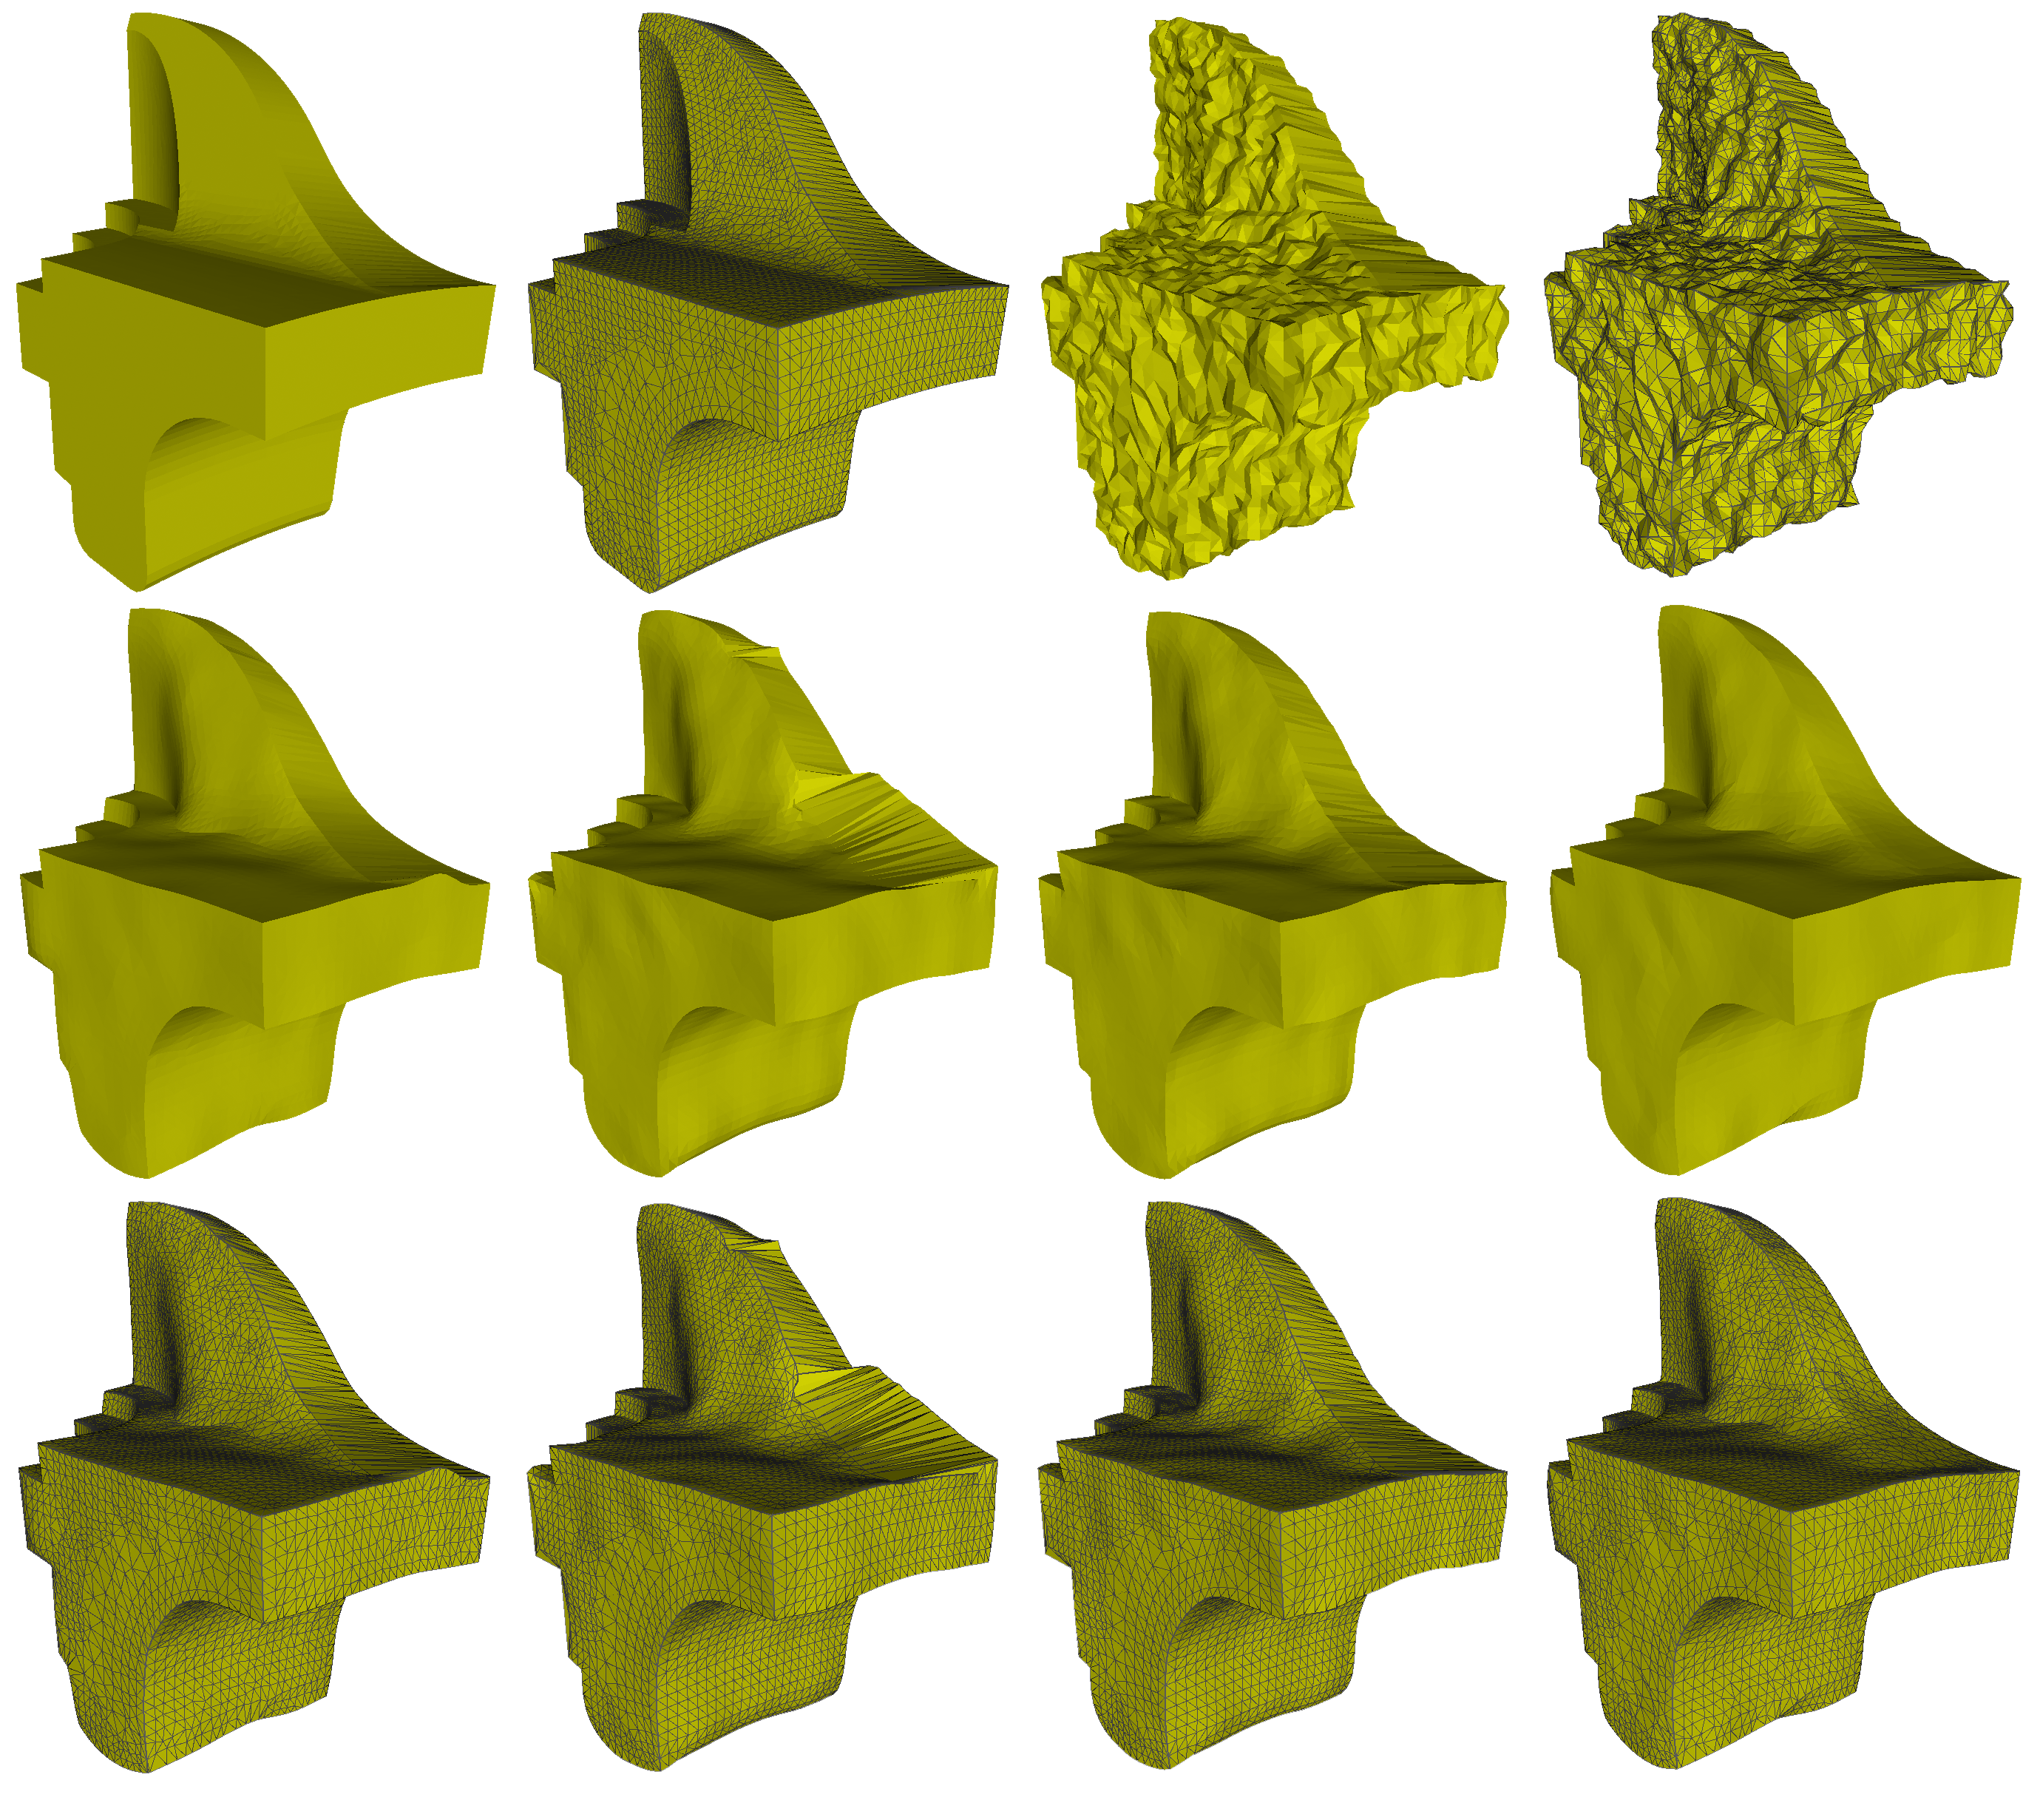
\includegraphics[width=16cm]{figuras/mechanic2_final.png}
\caption{Comparação da técnica proposta com as técnicas de \cite{zhang2015guided}, \cite{sun2007fast} e \cite{zheng2011bilateral} para o modelo \textit{mechanic}. Primeira linha: \textit{ground-truth}, \textit{ground-truth} com malha, modelo com ruído sintético, modelo com ruído sintético e malha. Segunda linha: técnicas de \cite{zhang2015guided}, \cite{sun2007fast}, \cite{zheng2011bilateral} e a técnica proposta, respectivamente. Terceira linha: as mesmas técnicas da linha anterior mostrando as malhas dos modelos.}
\label{fig:mechanic2_final}
\end{figure}

\clearpage






\begin{figure}[p]
\captionsetup{width=\linewidth}
\centering
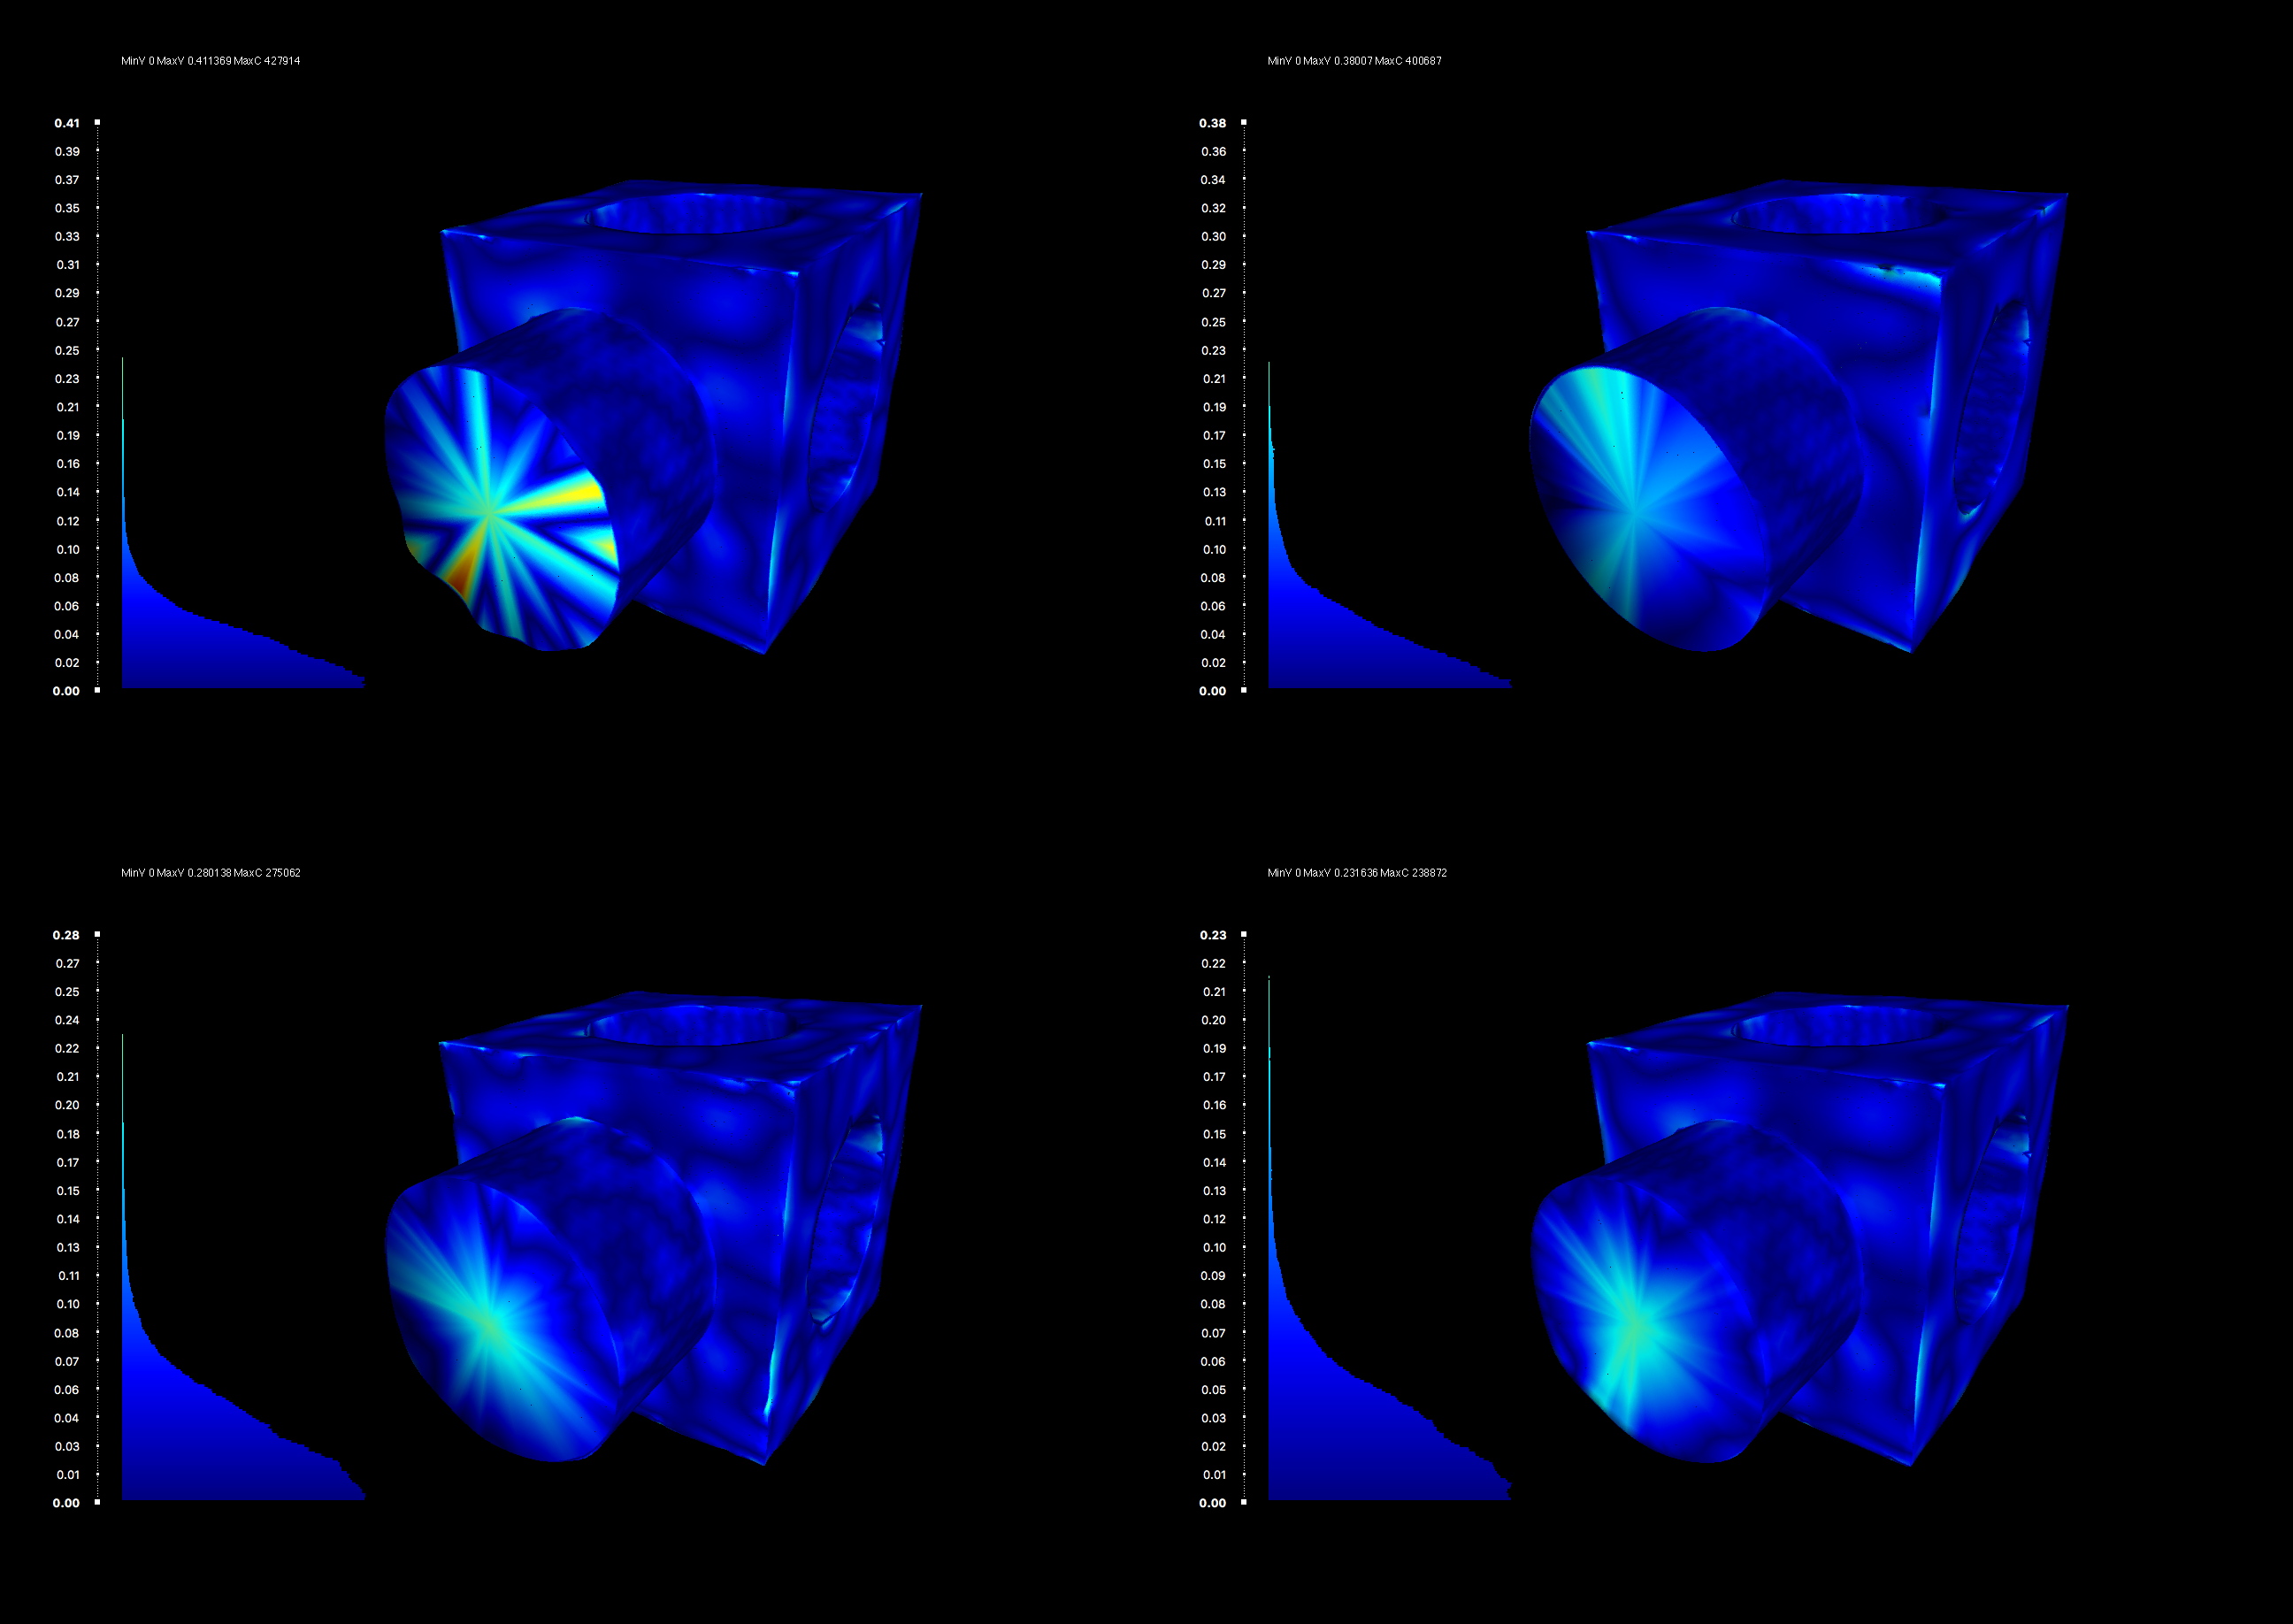
\includegraphics[width=16cm]{figuras/block_hausdorff_final.png}
\caption{Visualização do modelo \textit{block} e um histograma dos 6 milhões de pontos de amostragem e seus respectivos valores de distância de \textit{Hausdorff}. Primeira linha: técnicas de \cite{zhang2015guided} e \cite{sun2007fast}. Segunda linha: técnica \cite{zheng2011bilateral} e a técnica proposta.}
\label{fig:block_hausdorff_final}
\end{figure}

\clearpage


\begin{figure}[p]
\captionsetup{width=\linewidth}
\centering
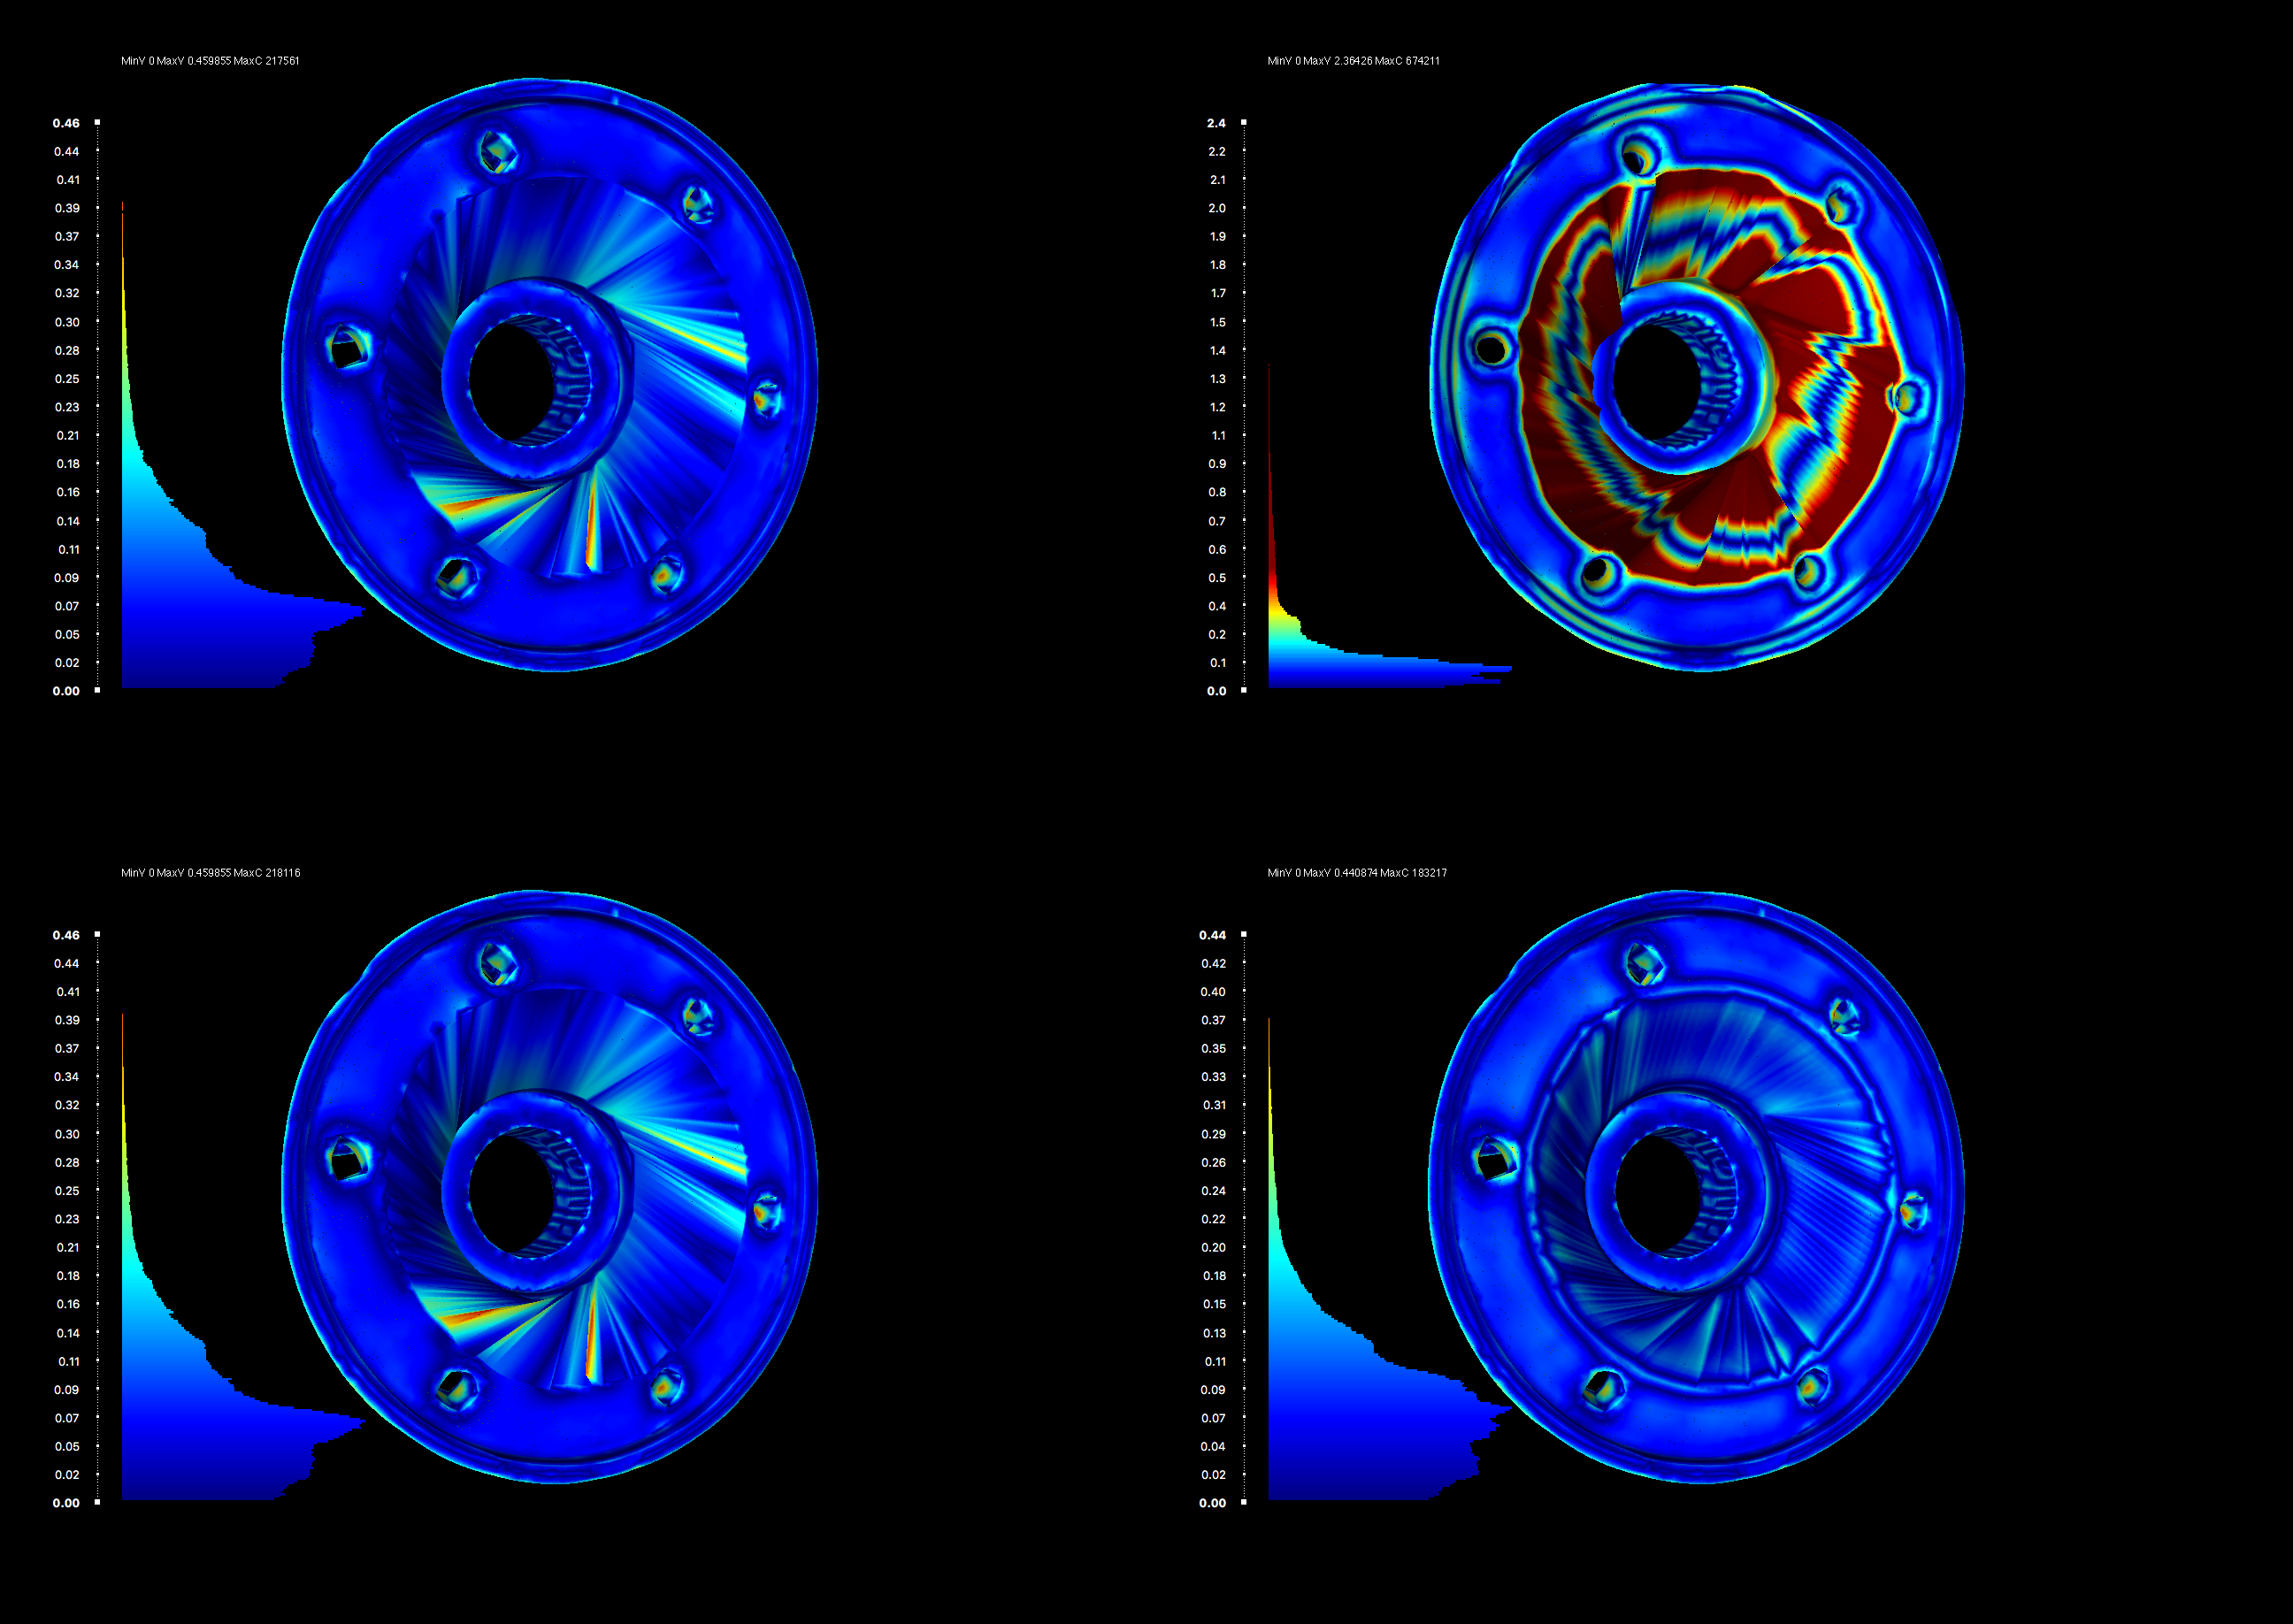
\includegraphics[width=16cm]{figuras/carter_hausdorff_final.png}
\caption{Visualização do modelo \textit{carter} e um histograma dos 6 milhões de pontos de amostragem e seus respectivos valores de distância de \textit{Hausdorff}. Primeira linha: técnicas de \cite{zhang2015guided} e \cite{sun2007fast}. Segunda linha: técnica \cite{zheng2011bilateral} e a técnica proposta.}
\label{fig:carter_hausdorff_final}
\end{figure}

\clearpage


\begin{figure}[p]
\captionsetup{width=\linewidth}
\centering
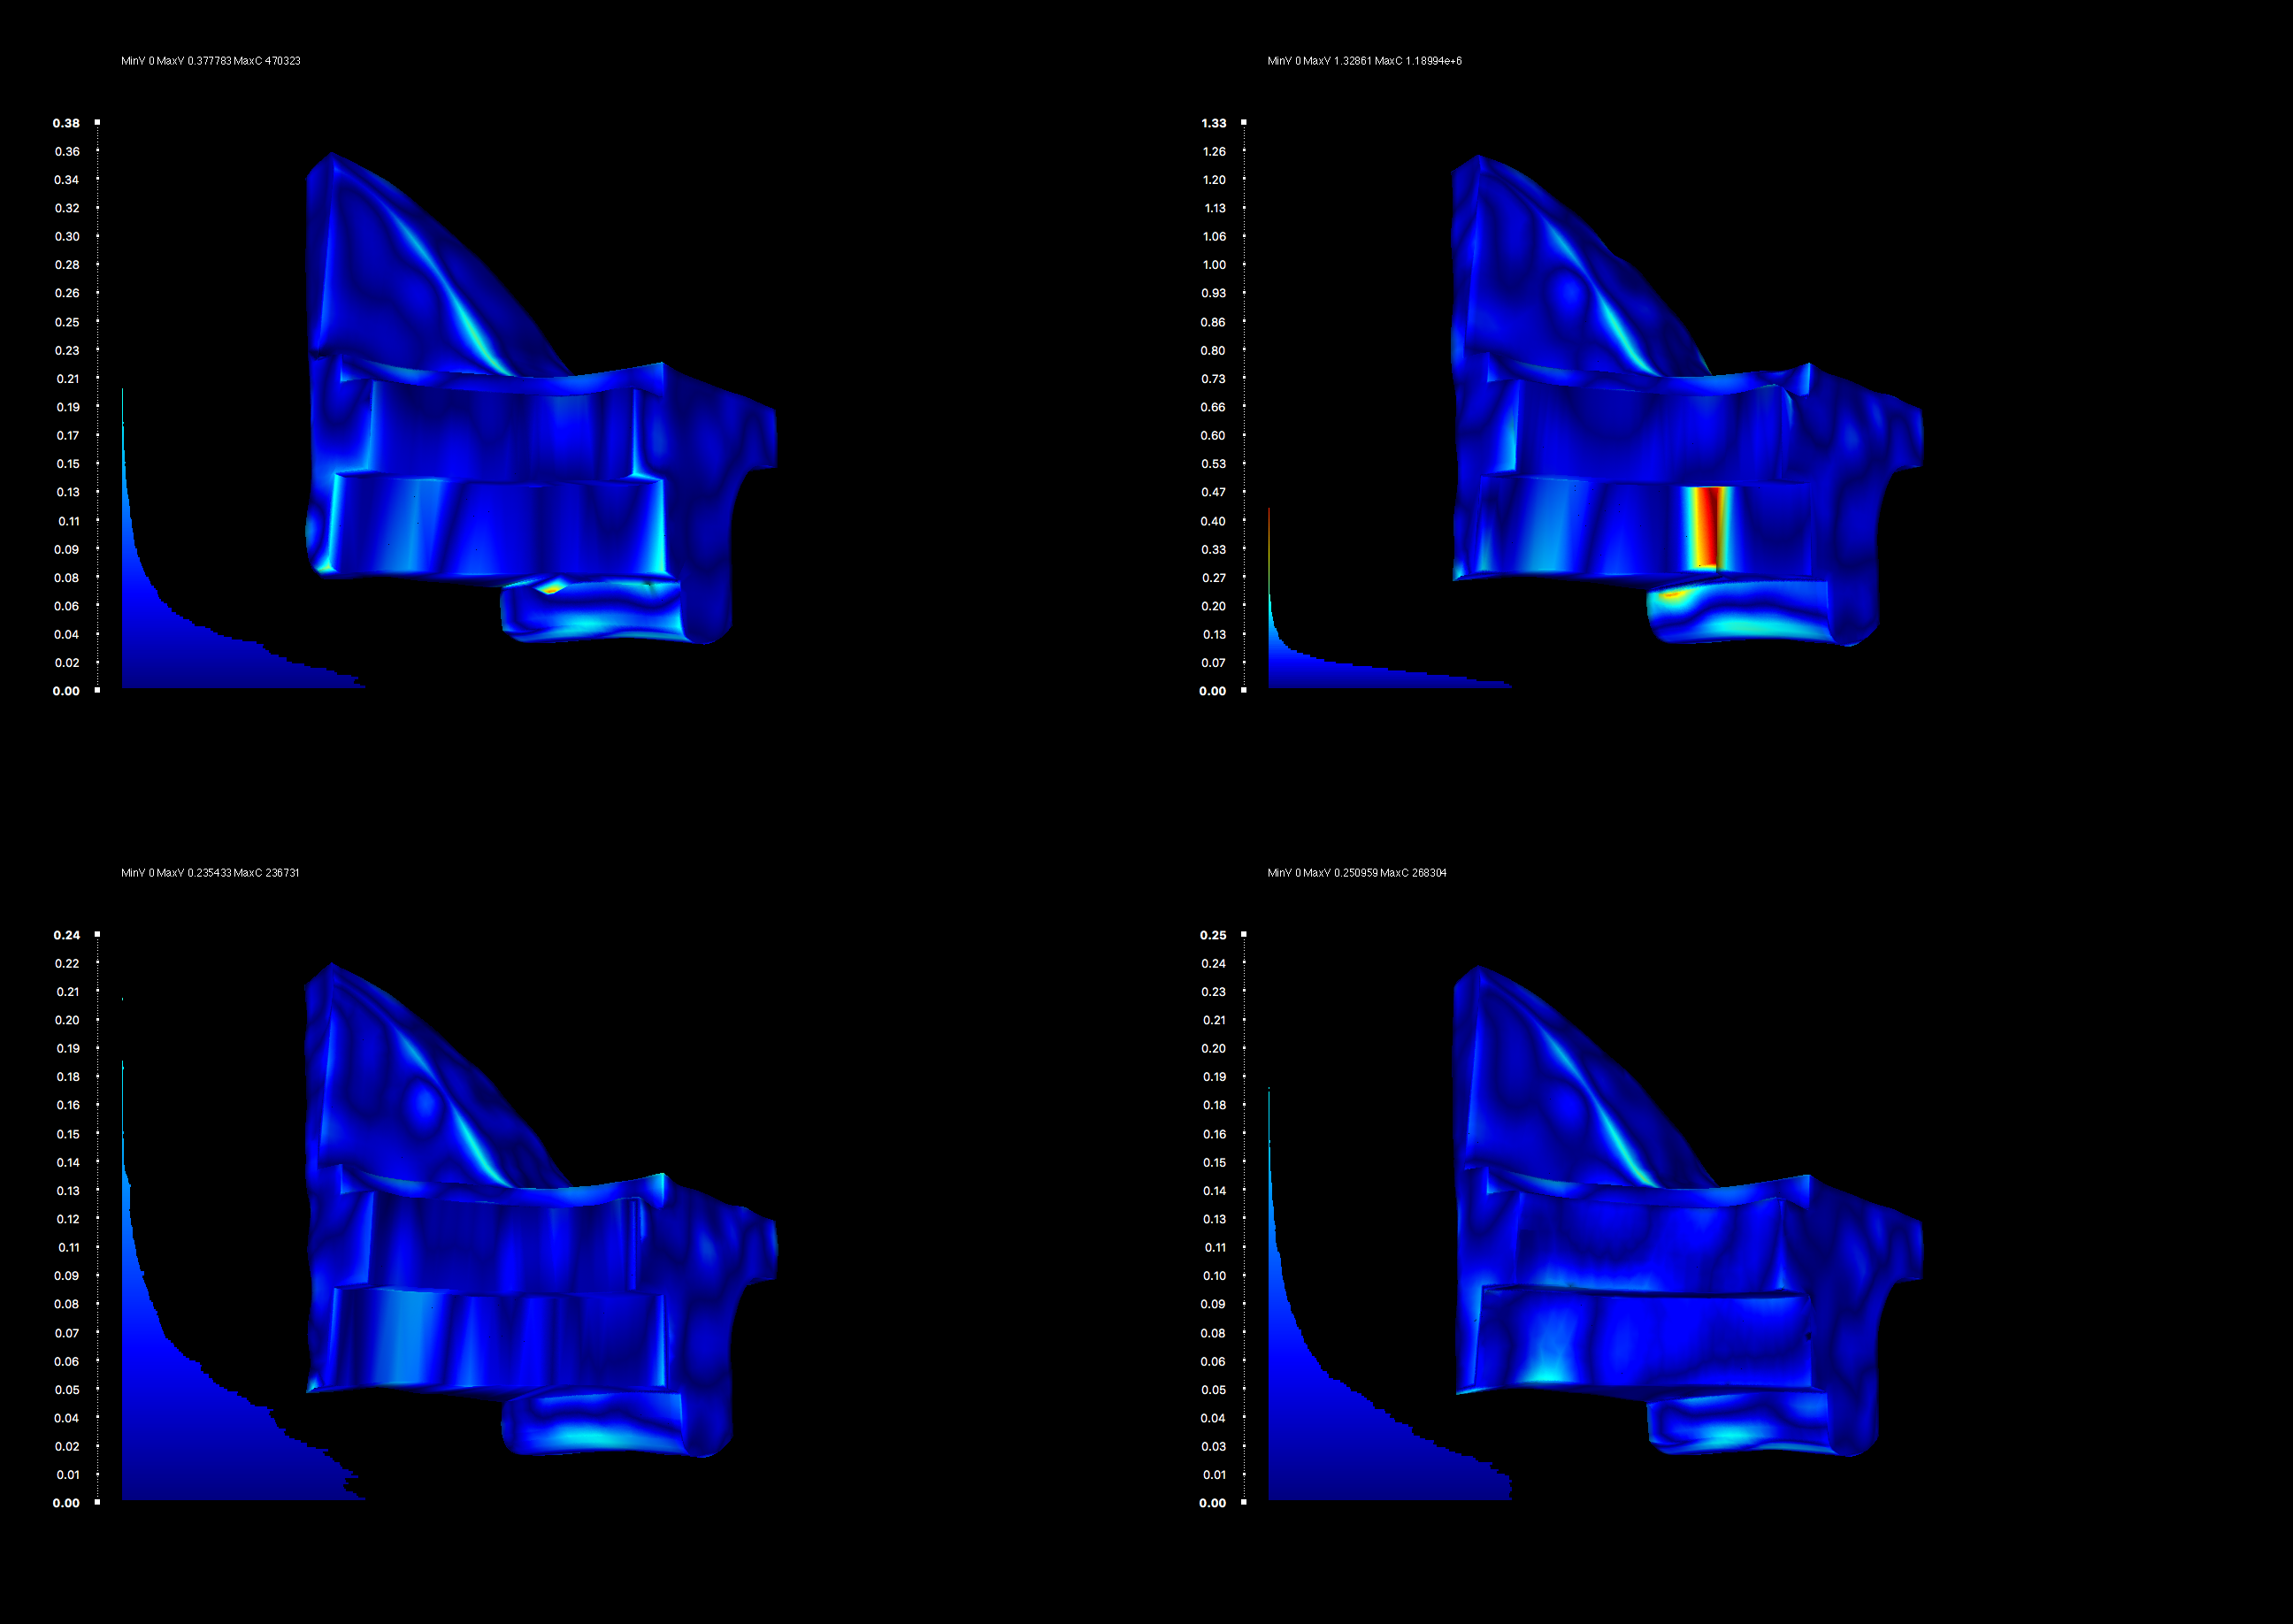
\includegraphics[width=16cm]{figuras/mechanic1_hausdorff_final.png}
\caption{Visualização do modelo \textit{mechanic} e um histograma dos 6 milhões de pontos de amostragem e seus respectivos valores de distância de \textit{Hausdorff}. Primeira linha: técnicas de \cite{zhang2015guided} e \cite{sun2007fast}. Segunda linha: técnica \cite{zheng2011bilateral} e a técnica proposta.}
\label{fig:mechanic1_hausdorff_final}
\end{figure}

\clearpage


\begin{figure}[p]
\captionsetup{width=\linewidth}
\centering
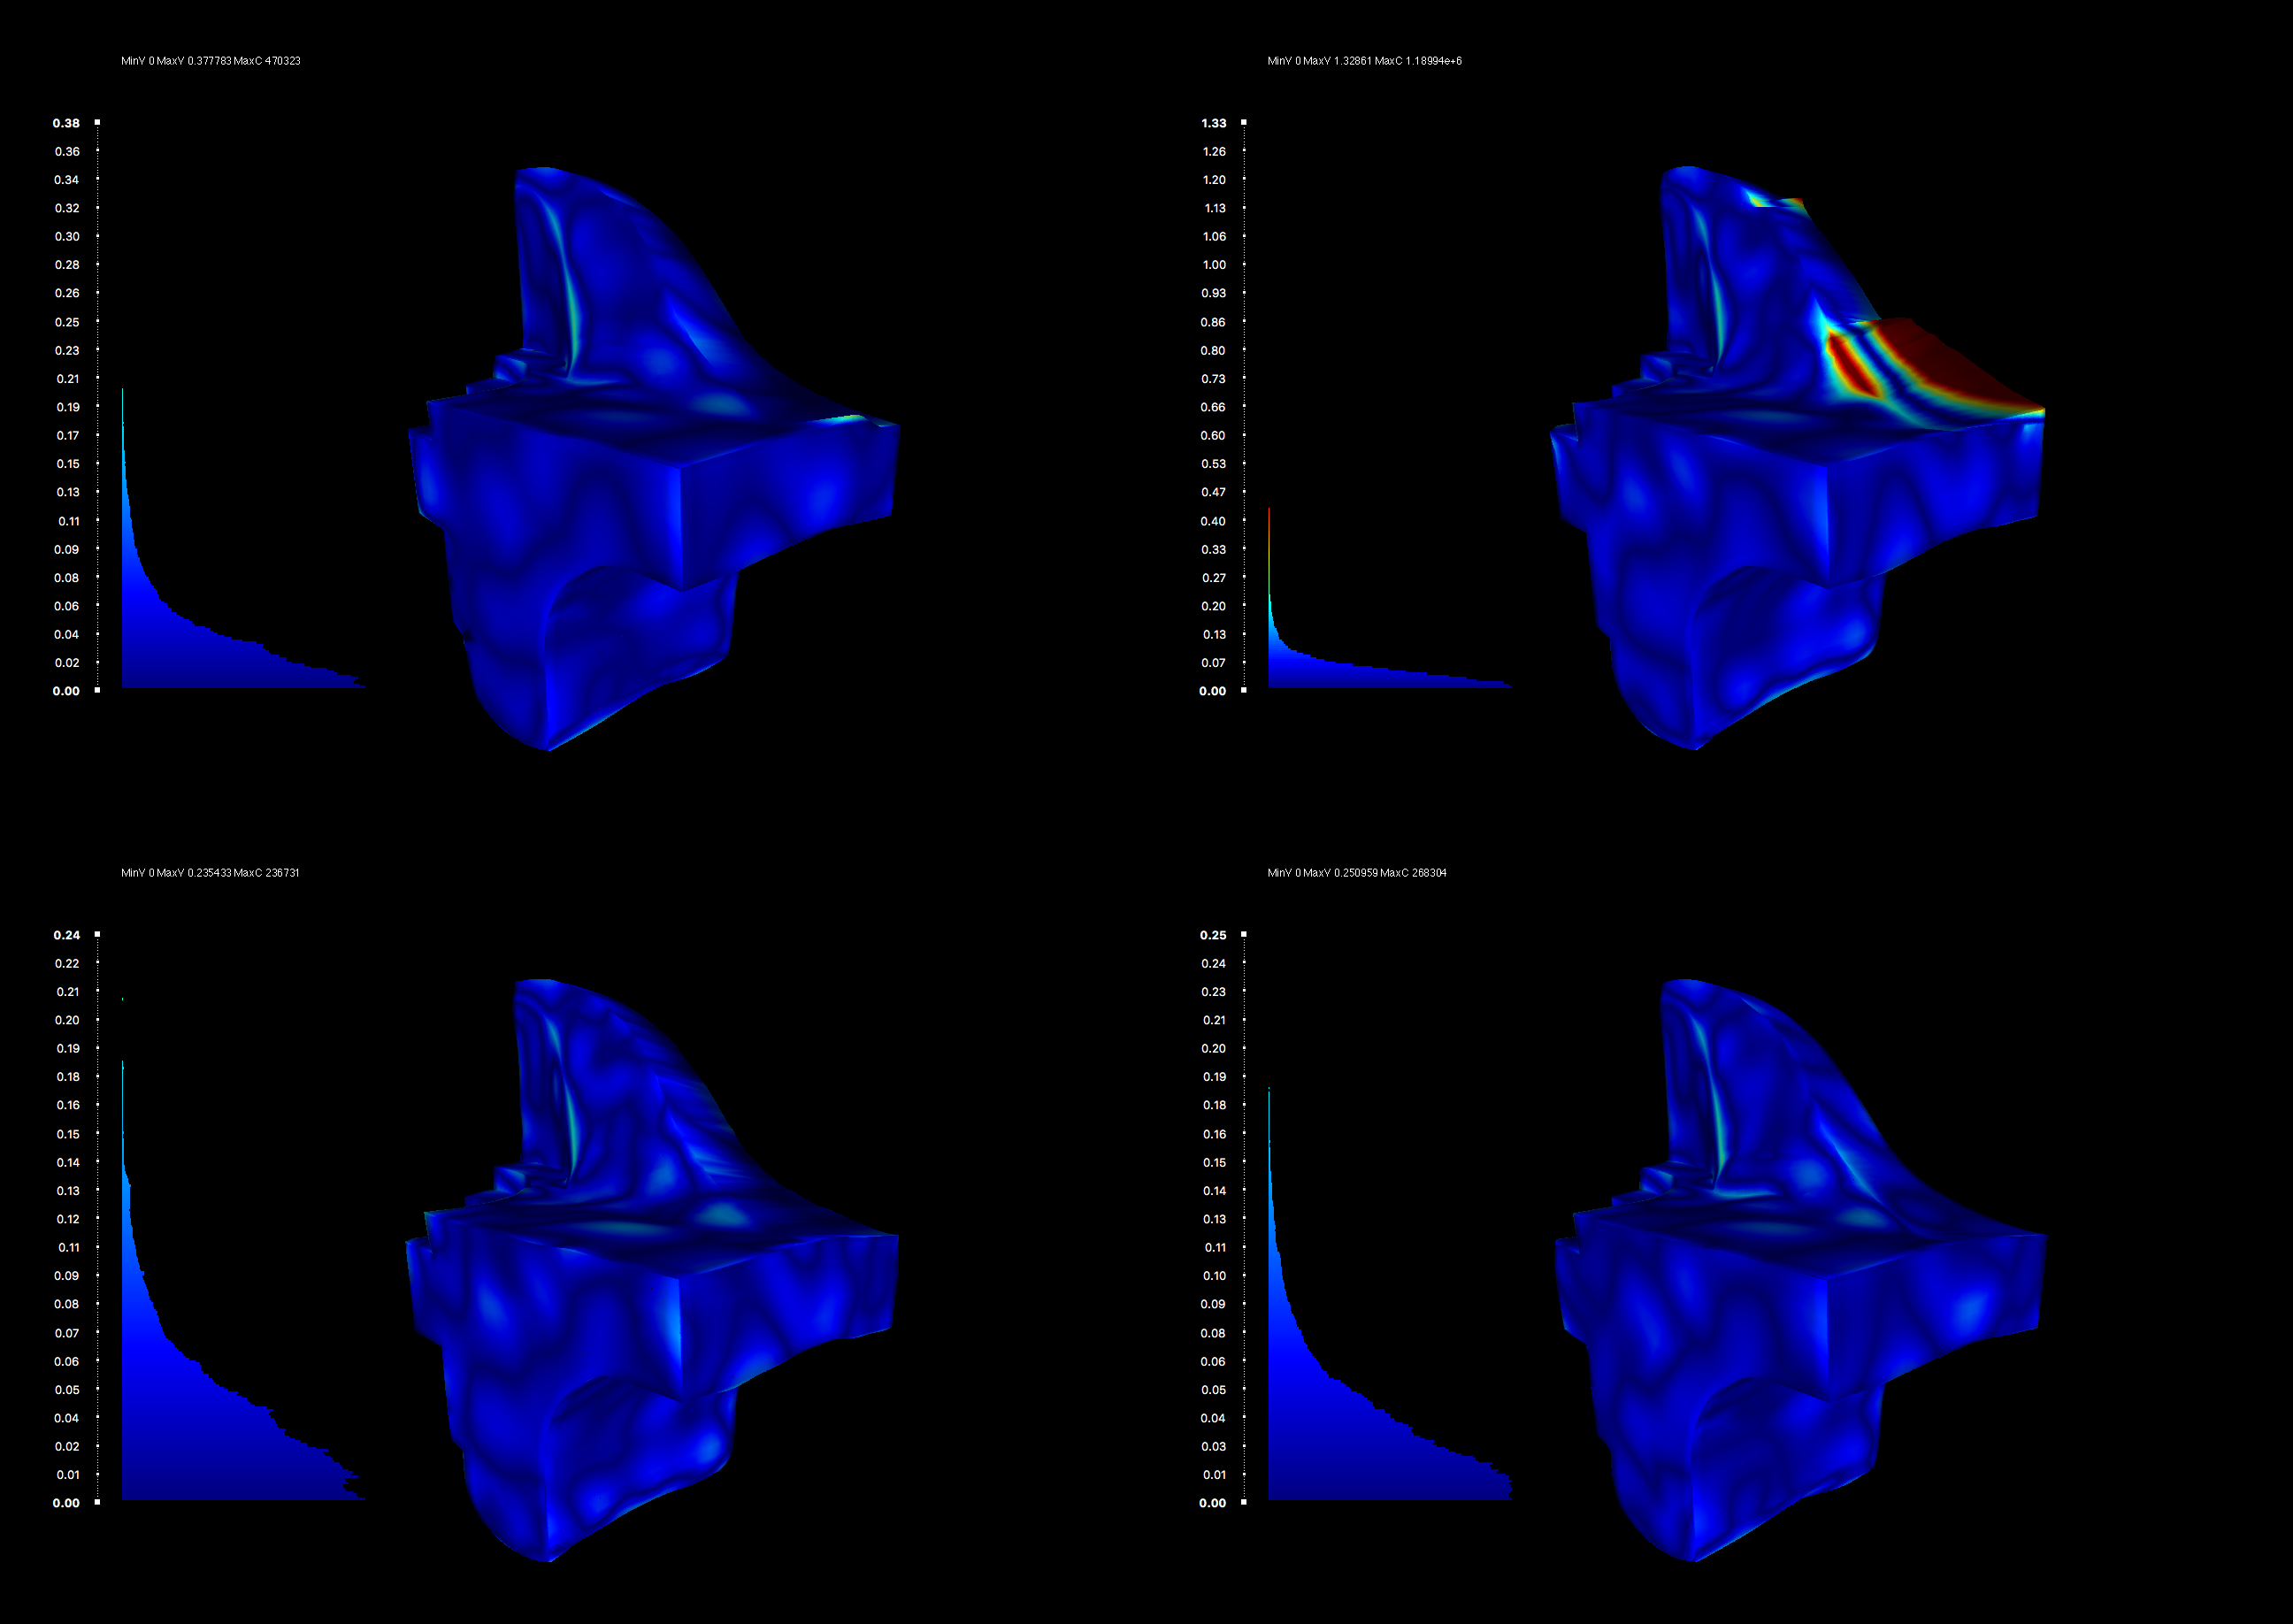
\includegraphics[width=16cm]{figuras/mechanic2_hausdorff_final.png}
\caption{Visualização do modelo \textit{mechanic} e um histograma dos 6 milhões de pontos de amostragem e seus respectivos valores de distância de \textit{Hausdorff}. Primeira linha: técnicas de \cite{zhang2015guided} e \cite{sun2007fast}. Segunda linha: técnica \cite{zheng2011bilateral} e a técnica proposta.}
\label{fig:mechanic2_hausdorff_final}
\end{figure}

\clearpage

\begin{figure}[!h]
\captionsetup{width=\linewidth}
\centering
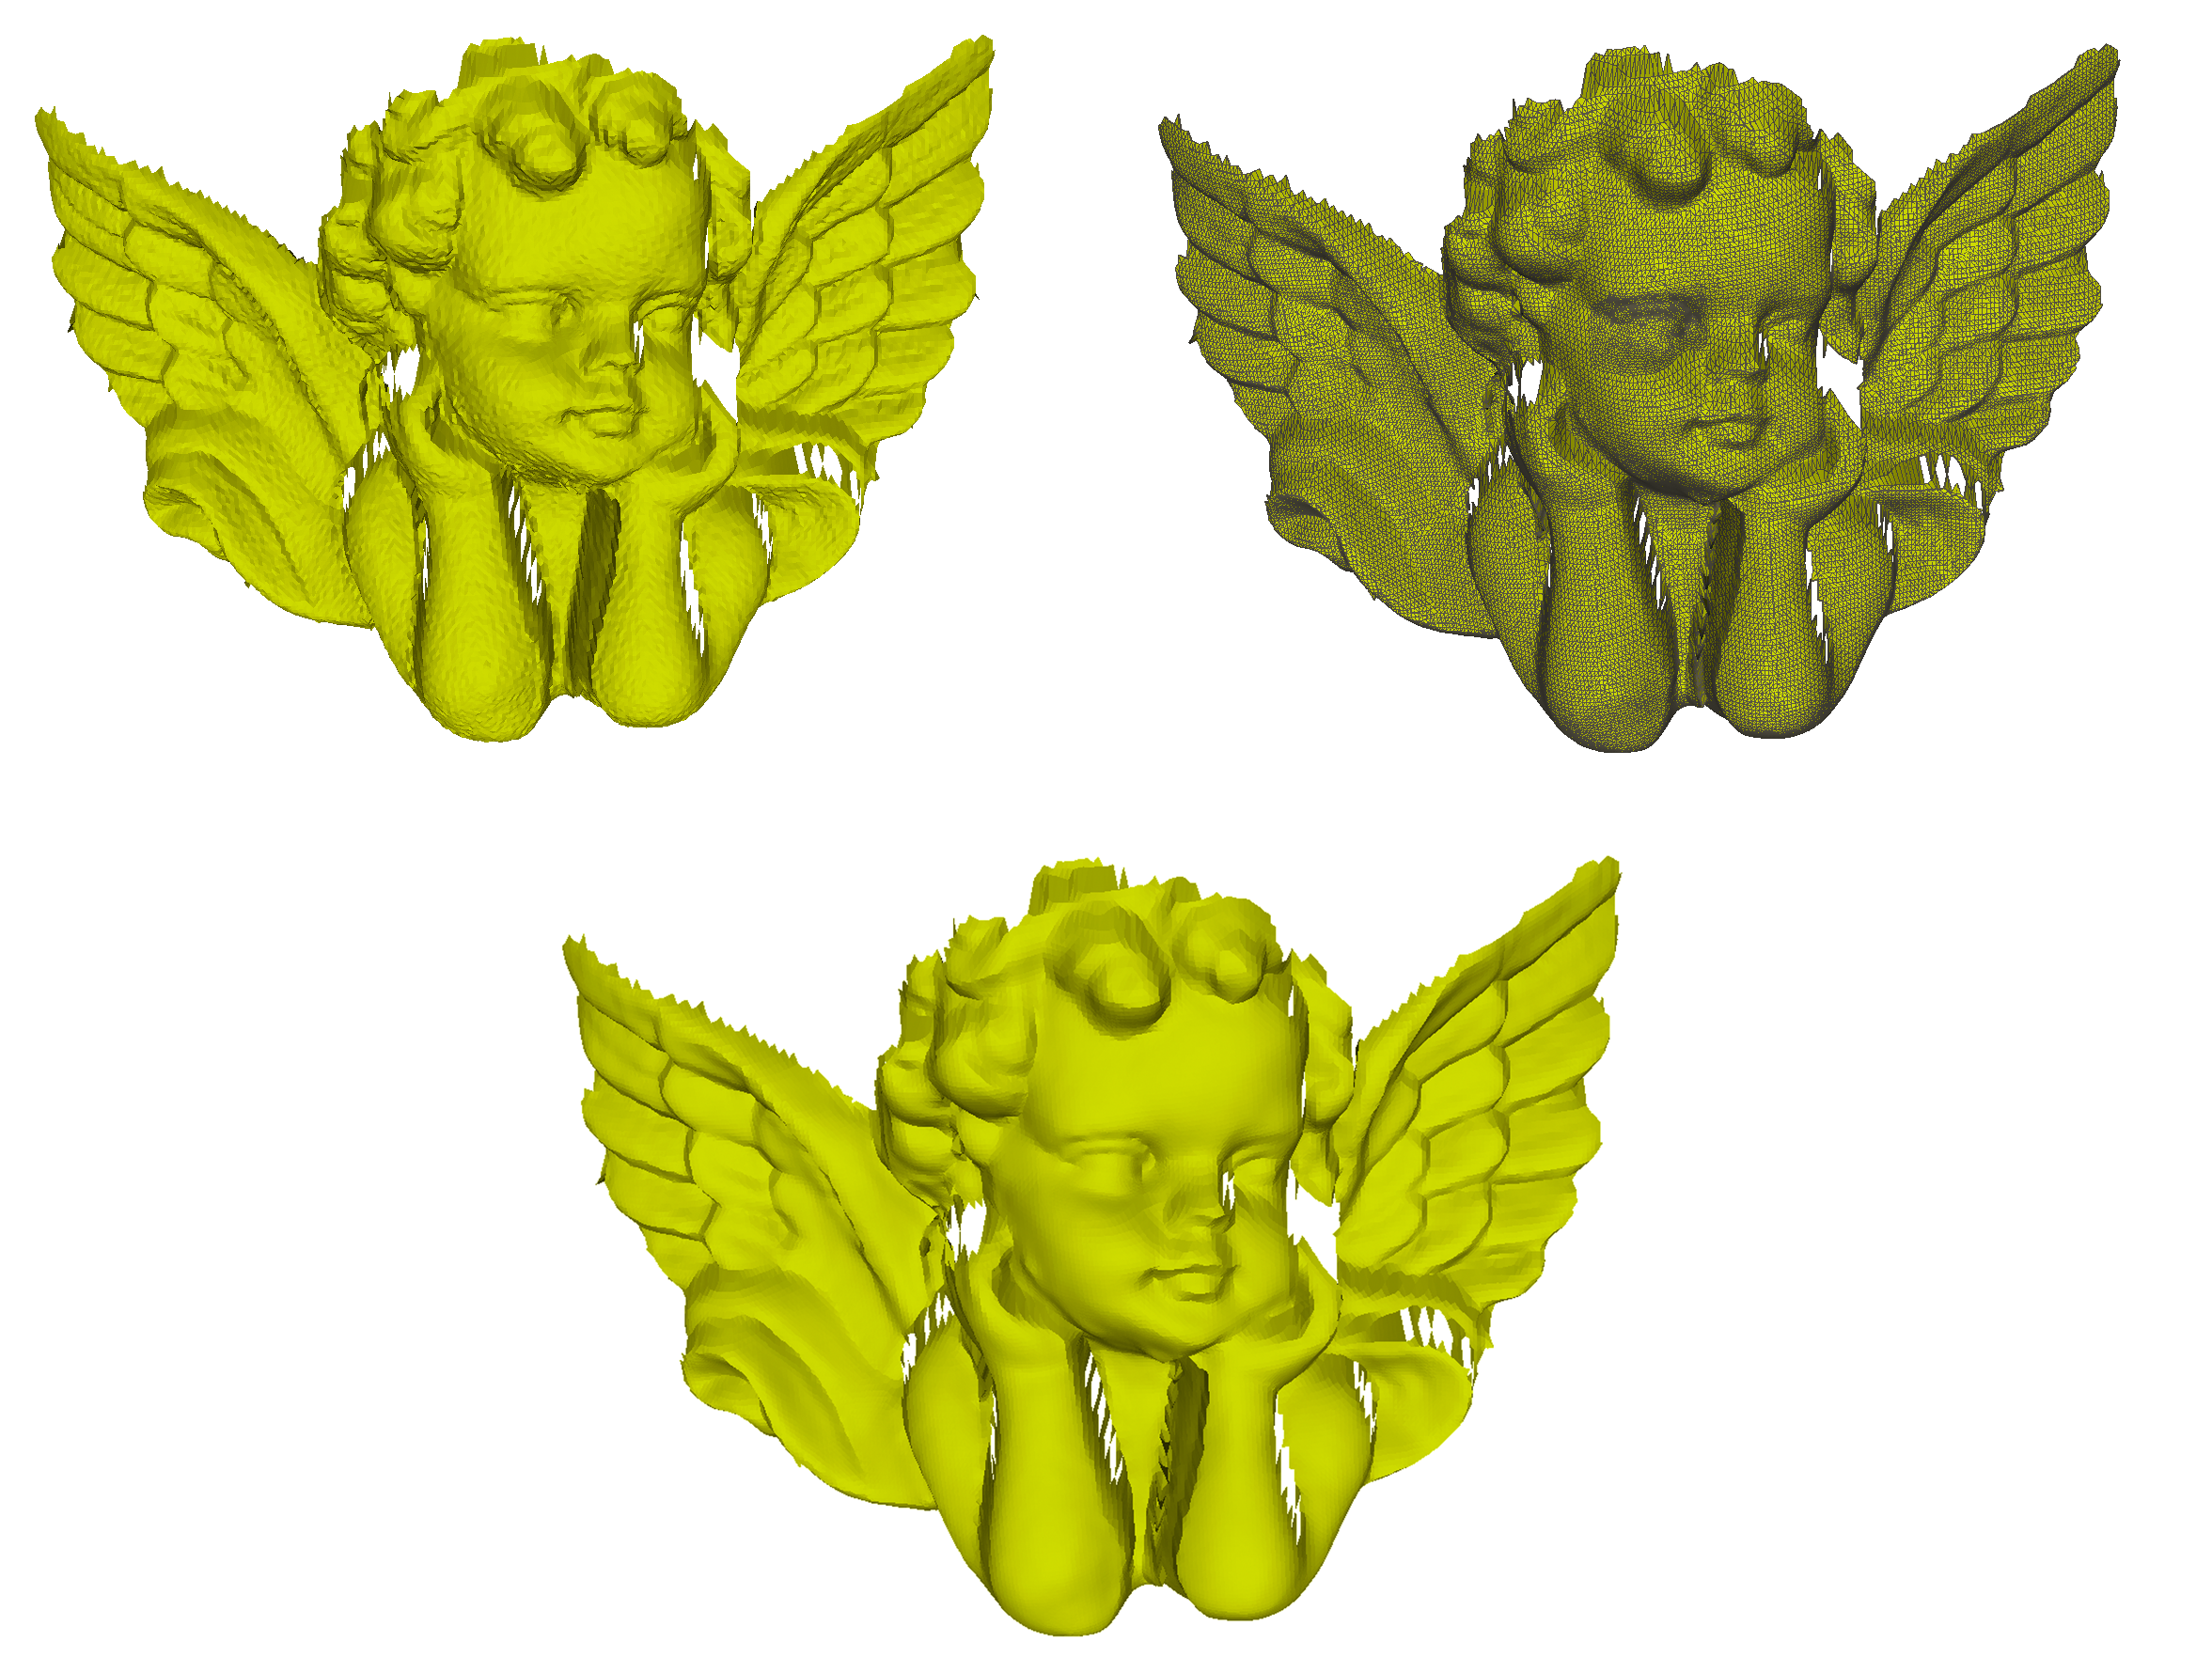
\includegraphics[width=\linewidth]{figuras/angel_final.png}
\caption{Técnica proposta utilizada no modelo \textit{angel}. Acima: modelo \textit{angel} com ruído e ao lado com ruído e malha. Abaixo: o resultado da técnica proposta aplicada ao modelo \textit{angel}.}
\label{fig:angel_final}
\end{figure}

\vspace{10mm}

\begin{figure}[!h]
\captionsetup{width=\linewidth}
\centering
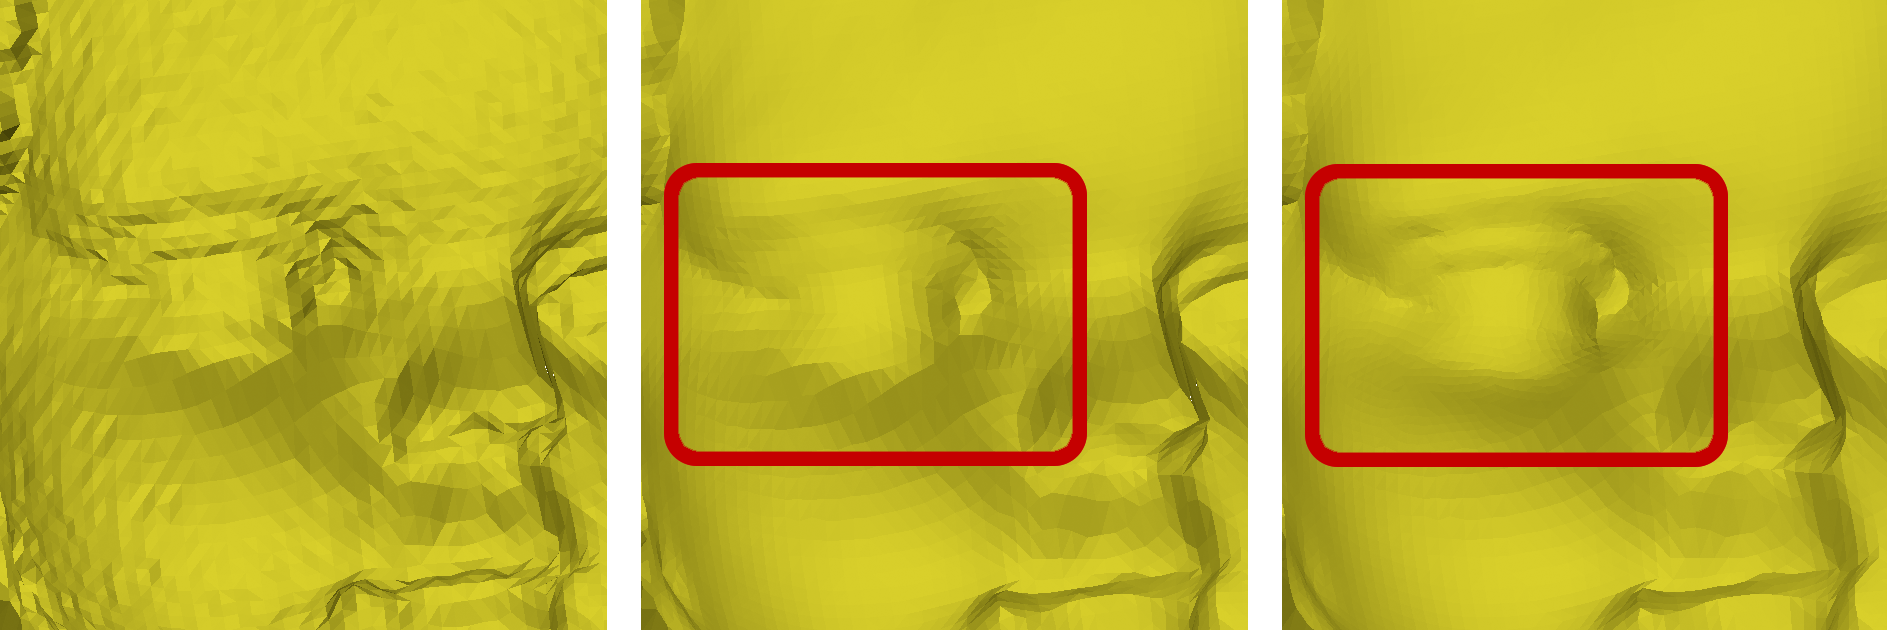
\includegraphics[width=\linewidth]{figuras/angel_detail.png}
\caption{Detalhe da região do olho do modelo \textit{angel}. Da esquerda para a direita: modelo \textit{angel} original com ruído, resultado da técnica proposta sem o passo de pré-processamento, resultado da técnica proposta com passo de pré-processamento.}
\label{fig:angel_detail}
\end{figure}


Pode-se notar, pelas figuras, que a técnica proposta obtém os melhores resultados para todos os modelos. Por fim, uma comparação dos valores das métricas para as quatro técnicas é mostrado na Tabela \ref{table:comparação_métricas}. A técnica proposta obtém melhores resultados para todos os modelos nas métricas mais importantes, obtendo o menor MMHD para todos os modelos apresentados. Em negrito são mostrados os melhores valores encontrados para cada modelo.

\begin{table}[]
\centering
\footnotesize
\renewcommand{\arraystretch}{1.3}
\caption{Comparação da técnica proposta com \cite{zhang2015guided}, \cite{sun2007fast} e \cite{zheng2011bilateral}.}
\setlength\tabcolsep{2pt}
\begin{tabular}{ |c|c|c|c|c|c| } 
\hline
Modelo & Métrica de Erro & \cite{zhang2015guided} & \cite{sun2007fast} & \cite{zheng2011bilateral} & Técnica Proposta \\
\hline
\hline

\multirow{5}{4em}{\centering \textit{Block}} 
& Sample Points & 6000000 & 6000000 & 6000000 & 6000000\\ 
\cline{2-6}
& MHD Mínimo & 0.0 & 0.0 & 0.0 & 0.0\\ 
\cline{2-6}
& MHD Máximo & 0.411390 & 0.380070 & 0.280138 & \textbf{0.231636}\\ 
\cline{2-6}
& \textbf{MMHD} & 0.032300 & 0.35615 & 0.033508 & \textbf{0.031509} \\ 
\cline{2-6}
& Proporção de Volume & 0.997919 & 0.997511 & \textbf{0.998231} & 0.9980328\\ 
\cline{1-6}

\multirow{5}{4em}{\centering \textit{Carter}} 
& Sample Points & 6000000 & 6000000 & 6000000 & 6000000\\ 
\cline{2-6}
& MHD Mínimo & 0.0 & 0.0 & 0.0 & 0.0\\ 
\cline{2-6}
& MHD Máximo & 0.459855 & 2.364260 & 0.459855 & \textbf{0.440874}\\ 
\cline{2-6}
& \textbf{MMHD} & 0.075780 & 0.164315 & 0.075759 & \textbf{0.075653} \\ 
\cline{2-6}
& Proporção de Volume & 1.06965 & \textbf{1.06304} & 1.06965 & 1.06701\\ 
\cline{1-6}

\multirow{5}{4em}{\centering \textit{Mechanic}} 
& Sample Points & 6000000 & 6000000 & 6000000 & 6000000\\ 
\cline{2-6}
& MHD Mínimo & 0.0 & 0.0 & 0.0 & 0.0\\ 
\cline{2-6}
& MHD Máximo & 0.377783 & 1.328610 & \textbf{0.235433} & 0.250672\\ 
\cline{2-6}
& \textbf{MMHD} & 0.032143 & 0.052403 & 0.033874 & \textbf{0.031893} \\ 
\cline{2-6}
& Proporção de Volume & 0.995846 & 1.00102 & \textbf{0.998717} & 0.997236 \\ 
\cline{1-6}

\hline
\end{tabular}
\label{table:comparação_métricas}
\end{table}
	\chapter{Conclusão e Trabalhos Futuros}
\label{chap:conclusao-e-trabalhos-futuros}

\section{Principais Contribuições} 
Esse trabalho apresentou uma técnica de otimização de malhas para remoção de ruídos de filtragem bilateral com pré-processamento. A técnica proposta apresenta bons resultados para qualquer tipo de modelo com ruído e ela possui um passo de pré-processamento que tem o objetivo de contribuir na otimização de, principalmente, modelos com ruídos que possuem qualidade de elementos excessivamente ruim.

Ao final deste trabalho foram apresentados, com ajuda de figuras, histogramas e tabelas, os resultados obtidos pela técnica proposta. Foi também mostrada a importância de melhorar a qualidade dos elementos de uma malha anteriormente à otimização propriamente dita. Conjuntamente, comparações foram apresentadas para mostrar o melhor desempenho da técnica proposta com o estado da arte em algoritmos de otimização de malhas para remoção de ruídos, em especial as técnicas descritas em \cite{zhang2015guided, sun2007fast, zheng2011bilateral}.

O trabalho proposto pode ser dividido basicamente em três etapas. A primeira consiste na análise e seleção de \textit{patches} de elementos. A segunda constitui-se do \textit{remalhamento} dos \textit{patches} selecionados, convertendo essas regiões em áreas com uma melhor qualidade de elementos. A terceira e última etapa consiste na filtragem das normais da malha seguido da atualização de seus vértices. Essa última etapa é reproduzida iterativamente até um resultado satisfatório (cerca de 10 a 15 iterações dependendo do modelo).

As principais contribuições deste trabalho são a apresentação de uma nova técnica de otimização de malhas para remoção de ruídos, que também melhora a qualidade de seus elementos, e a confirmação da importância que a melhoria local da qualidade dos elementos da malha produz no resultado de uma técnica de otimização de malhas com intuito de remoção de ruídos.

\section{Trabalhos Futuros}

A técnica aqui apresentada possui três etapas principais. Na primeira etapa foi utilizado um julgamento visual por parte do usuário, onde ele escolhe as regiões a serem \textit{remalhadas}. Uma investigação mais aprofundada deverá ser realizada no intuito da automatização desse processo, onde métricas de qualidade de triângulos poderão ser usadas para saber quais regiões da malha entrarão no processo de \textit{remalhamento}. 

Na segunda etapa, o algoritmo de \cite{miranda2009surface} foi utilizado. Algumas outras opções como \cite{attene2013polygon, zhao2007robust} também poderão ser testadas, pois talvez possam produzir resultados ainda melhores para reconstrução de malhas. No entanto, no trabalho proposto há a existência de uma malha suporte, fazendo com que o \textit{remalhamento} siga exatamente essa malha suporte, sendo portanto muito improvável que os resultados utilizando as técnicas de \cite{attene2013polygon, zhao2007robust}, que predizem por onde a reconstrução deve seguir, superem os resultados já apresentados no Capítulo \ref{chap:exemploseresultados}. Um estudo mais detalhado, com comparações e implementações, deve ser realizado para este passo.

Na última etapa, um algoritmo de filtragem das normais e atualização de vértices é proposto baseado em \cite{zhang2015guided}. Mais algumas comparações podem ser realizadas utilizando outras técnicas de otimização de malha neste passo, estendendo, dessa forma, a técnica proposta a uma técnica geral de pré-processamento para otimização de malhas, onde qualquer algoritmo de otimização pode ser configurado. Essa extensão não é algo trivial, necessitando de estudos mais aprofundados.


	
	%Elementos pós-textuais	
	\bibliography{3-pos-textuais/referencias}
%	\imprimirglossario	
% 	\imprimirapendices
% 		% Adicione aqui os apendices do seu trabalho
% 		% \apendice{Exemplo de apêndice}
% \label{ap:A}

% Um apêndice é um documento elaborado pelo autor, diferentemente do anexo. Geralmente, se coloca como apêndice, questionários, códigos de programação, tabelas que tomariam muito espaço no meio do trabalho. Artigos, resumos ou qualquer publicação relacionada ao trabalho podem ser utilizados como apêndice.
% 		% \apendice{Questionário utilizado para...}
% \label{ap:B}

% \begin{questao}
% 	\item Esta é a primeira questão com alguns itens:
% 		\begin{enumerate}
% 			\item Este é o primeiro item
% 			\item Segundo item
% 		\end{enumerate}
% 	\item Esta é a segunda questão:
% 		\begin{enumerate}
% 			\item Este é o primeiro item
% 			\item Segundo item
% 		\end{enumerate}
% 	\item Lorem ipsum dolor sit amet, consectetur adipiscing elit. Nunc dictum sed tortor nec viverra. consectetur adipiscing elit. Nunc dictum sed tortor nec viverra.
% 		\begin{enumerate}
% 			\item consectetur
% 			\item adipiscing
% 			\item Nunc
% 			\item dictum
% 		\end{enumerate}
% \end{questao}

% 		% \apendice{Códigos-fontes utilizados para...}
% \label{ap:C}

% \lstinputlisting[language=C++,caption={Hello World em C++}]{figuras/main.cpp}


% \begin{lstlisting}[language=Java,caption={Hello World em Java}]
% public class HelloWorld {
% 	public static void main(String[] args) {
% 		System.out.println("Hello World!");
% 	}
% }
% \end{lstlisting}


% 		% \apendice{\textit{IEEE CEFC 2016}}
% \label{ap:D}

% \textit{Digest} submetido ao \textit{The 17th Biennial Conference on Eletromagnetic Field Computation, Miami FL - NOV 13-16, 2016, USA}.

% %Código fonte para inserir um arquivo em PDF
% 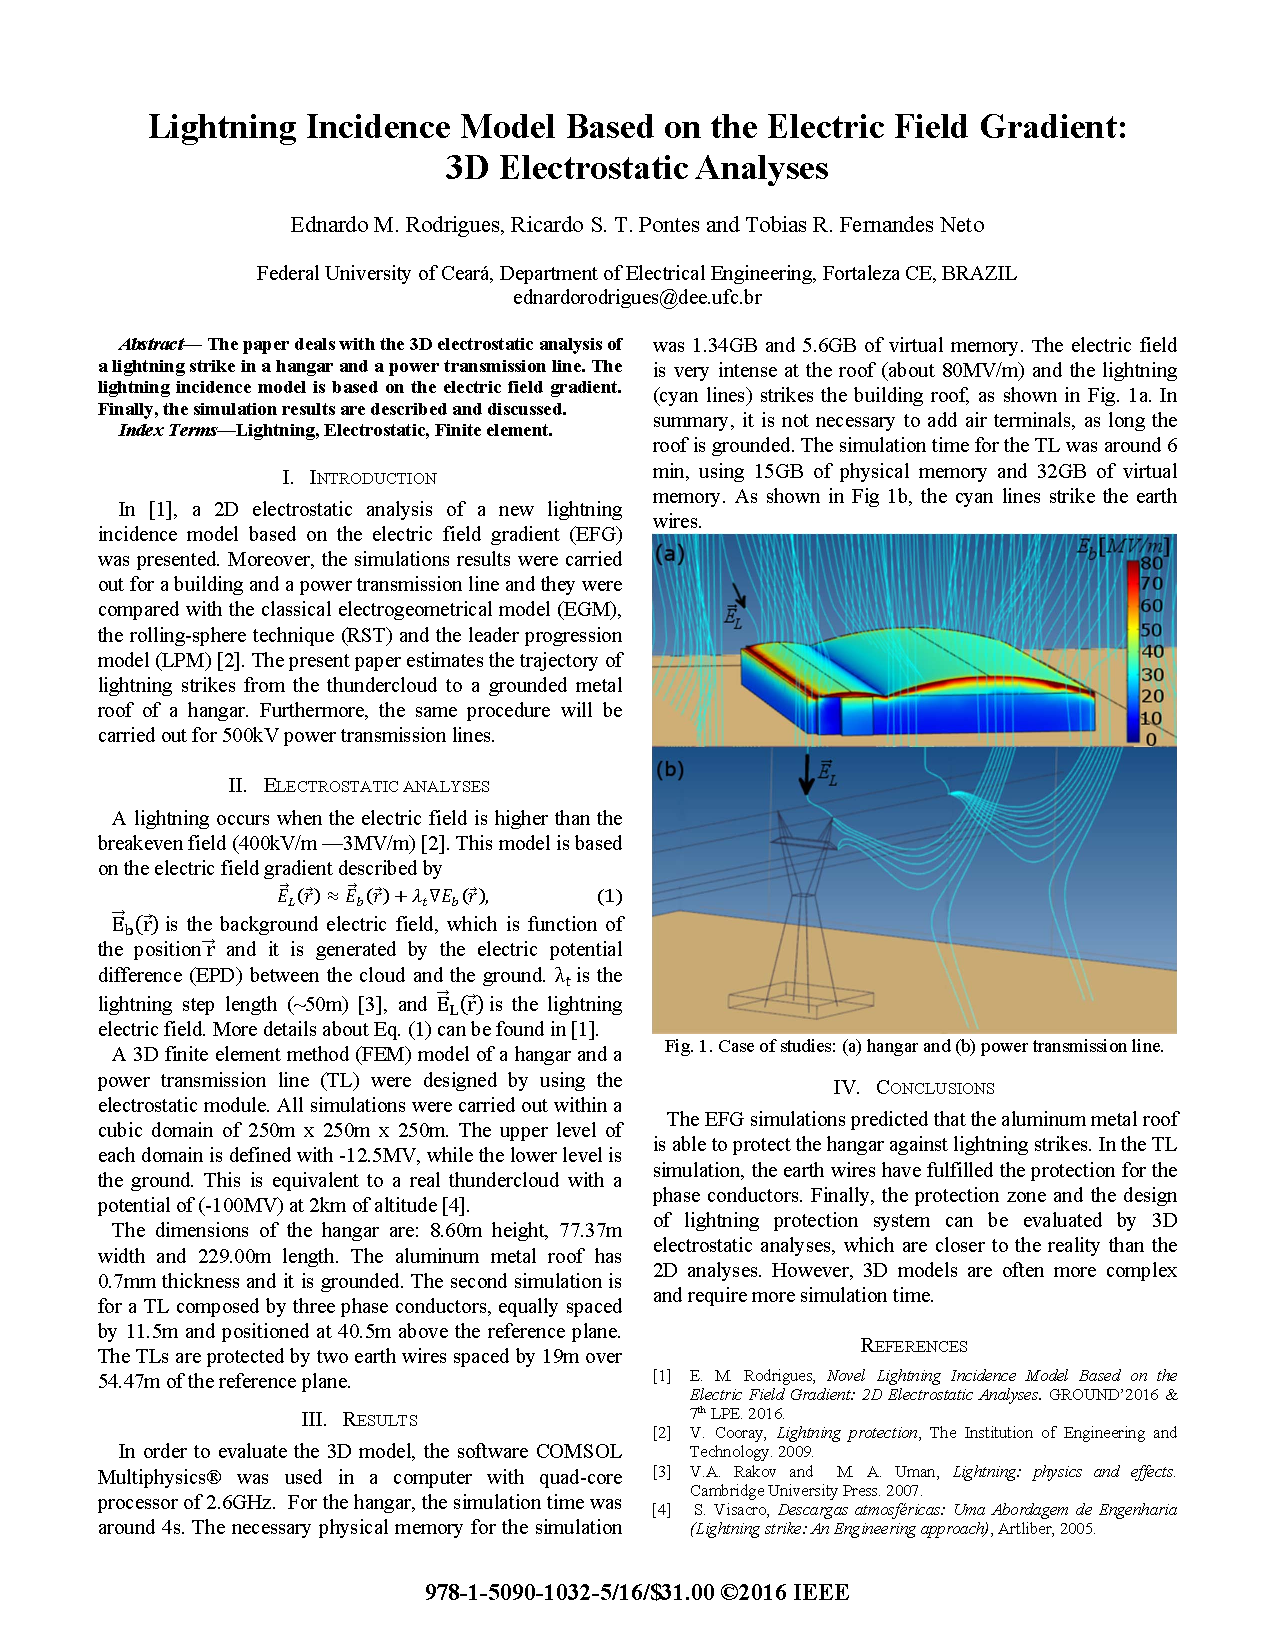
\includepdf[pages={-}]{3-pos-textuais/apendices/PID4416093.pdf}
% 	\imprimiranexos
% 		% Adicione aqui os anexos do seu trabalho
% 		\anexo{Exemplo de um anexo}
\label{an:ex_anexo_a}

Um anexo é um documento que não foi elaborado pelo autor, ou seja, o autor apenas anexa. Anexos podem ser tabelas, mapas, diagramas, \textit{datasheets}, manuais e etc. 




% 		\anexo{Exemplo de um anexo em PDF}
\label{an:ex_anexo_b}

O autor pode anexar um \gls{PDF}, traduzido como formato portátil de documento. Veja o código fonte utilizado para anexar o arquivo ``Sikasil.pdf'' que foi colocado dentro da pasta ``anexos'' que por sua vez está dentro da pasta ``elementos-pos-textuais''. Tenha muita atenção na hora de especificar o local do arquivo. Recomenda-se não utilizar caracteres especiais para nomear pastas e, principalmente, arquivos. 

Pode-se fazer uma descrição sucinta do arquivo anexado.

%Comando para incluir um arquivo em PDF:
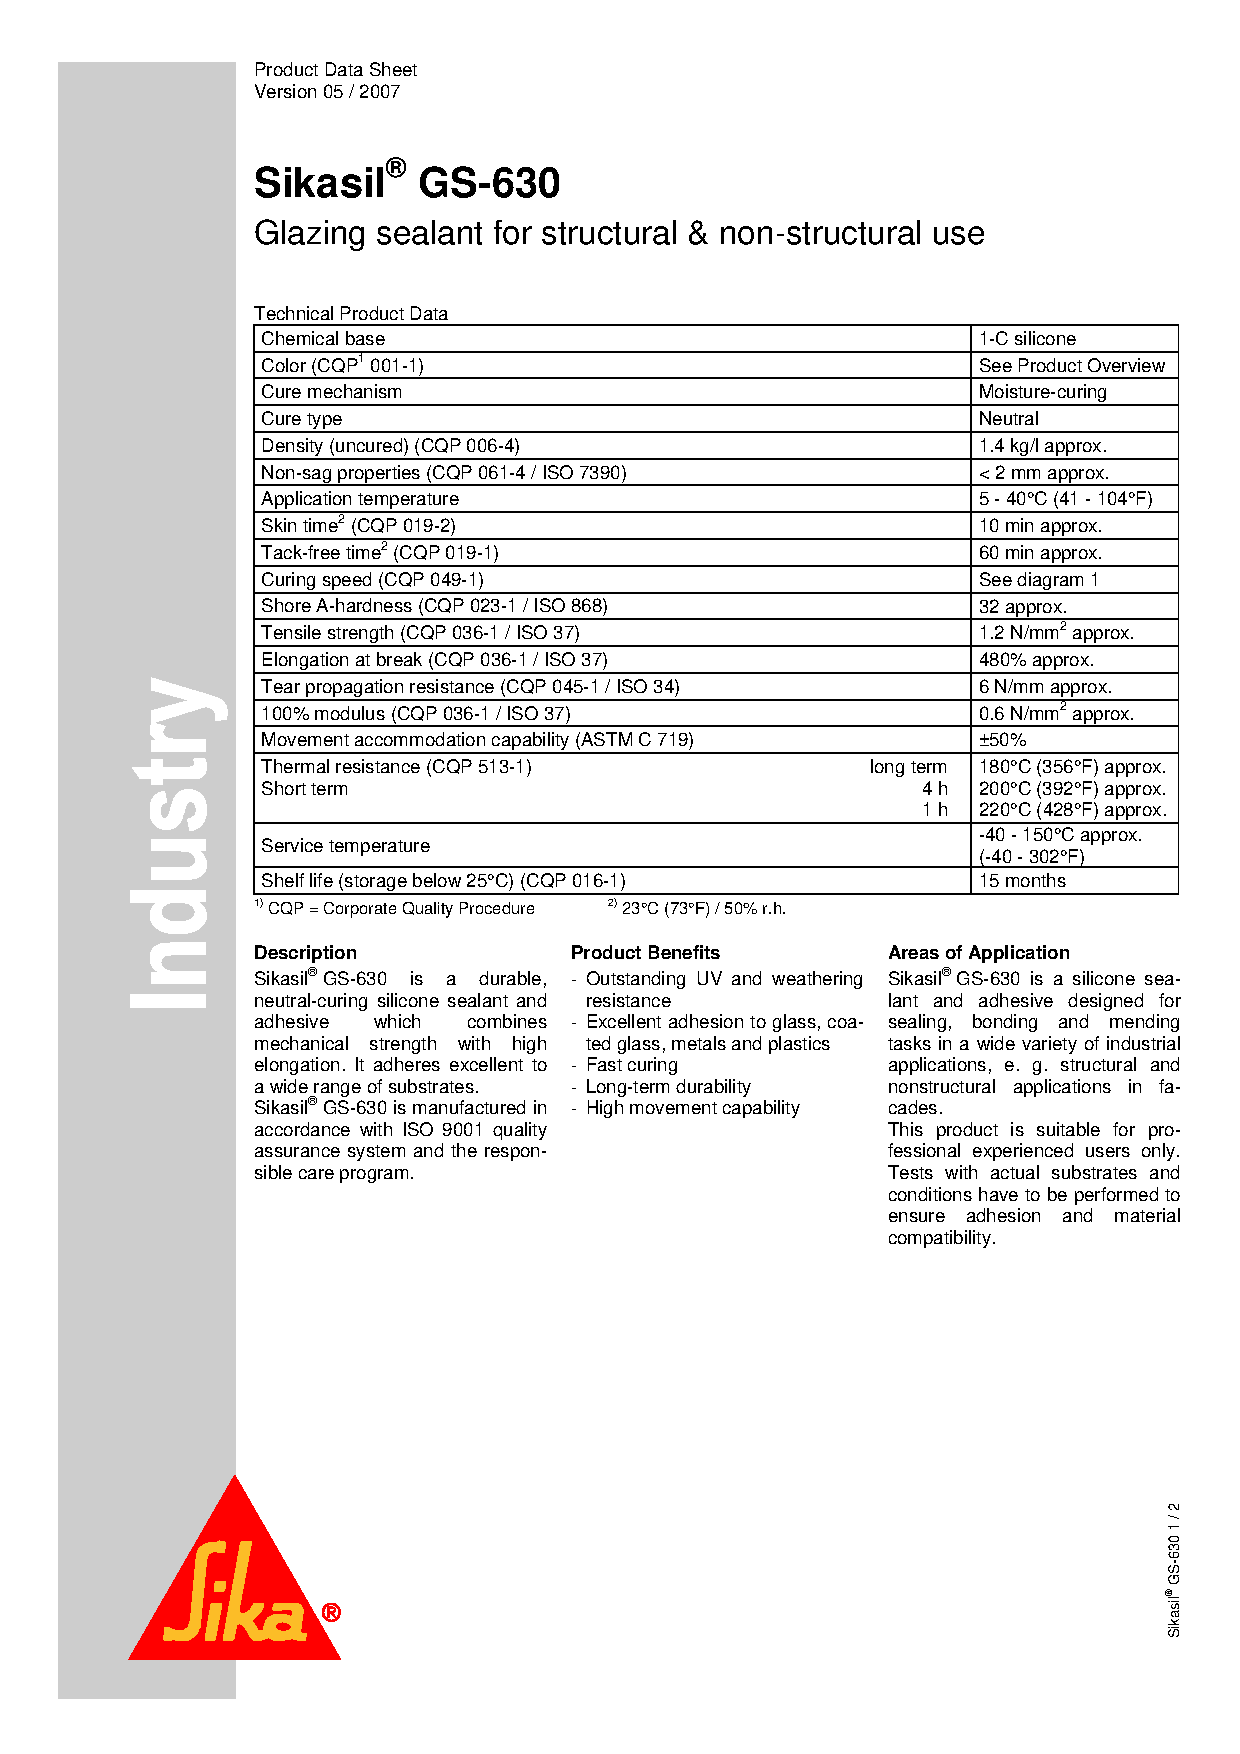
\includepdf[pages={-}]{3-pos-textuais/anexos/Sikasil.pdf}

		
% 	\imprimirindice

\end{document}